\documentclass{bukumjh}

\begin{document}

\frontmatter

\insertsampuldalam
\insertcopyrightpage
\insertkatapengantar

\begin{center}
\Large {\jsg Rencana Pembelajaran Semester (RPS)} \\[0.2cm]
\large Mata Kuliah: {\jsg Pemodelan Matematika} \\
Program Studi Matematika – Semester 7 \\
\end{center}

\section*{Identitas Mata Kuliah}
\begin{tabular}{ll}
Kode Mata Kuliah & MAT61730 \\
Bobot & 3 SKS \\
Semester & 7 \\
Dosen Pengampu & Dr. Mohammad Jamhuri, M.Si. \\
\end{tabular}

\section*{Deskripsi Mata Kuliah}
Mata kuliah ini membahas konsep, metode, dan aplikasi pemodelan matematika untuk berbagai fenomena nyata di bidang sains, teknik, ekonomi, dan sosial. Mahasiswa akan belajar bagaimana membangun model dari fenomena, melakukan analisis, menyelesaikan model secara analitik atau numerik, serta menginterpretasikan hasilnya. 

\section*{Capaian Pembelajaran Mata Kuliah (CPMK)}
Setelah mengikuti perkuliahan ini, mahasiswa mampu:
\begin{enumerate}
    \item Menjelaskan konsep dasar pemodelan matematika.
    \item Merumuskan model matematika dari fenomena nyata.
    \item Menganalisis dan menyelesaikan model dengan metode analitik maupun numerik.
    \item Menginterpretasikan hasil model dan mengaitkannya dengan konteks masalah.
    \item Menggunakan perangkat lunak komputasi (Python/Matlab) untuk simulasi model.
\end{enumerate}

\section*{Bahan Kajian dan Rencana Pertemuan}
\begin{tabularx}{\textwidth}{|c|X|p{2.5cm}|}
\hline
{\jsg Week} & {\jsg Materi} & {\jsg Metode} \\ \hline
1 & Pengantar pemodelan matematika: definisi, tipe model, langkah pemodelan. Contoh kasus sederhana (pertumbuhan populasi). & Ceramah, diskusi, latihan \\ \hline
2 & Model pertumbuhan populasi: eksponensial, logistic. & Ceramah, diskusi, latihan \\ \hline
3 & Model predator-prey Lotka–Volterra. & Ceramah, simulasi komputer \\ \hline
4 & Model epidemiologi: SIR, SEIR. & Ceramah, simulasi komputer \\ \hline
5 & Model antrian (queueing models). & Ceramah, diskusi, studi kasus \\ \hline
6 & Rantai Markov: cuaca, produksi, permainan. & Ceramah, diskusi, simulasi \\ \hline
7 & Model input-output Leontief dalam ekonomi. & Ceramah, diskusi, latihan \\ \hline
{\jsg 8} & {\jsg Ujian Tengah Semester (UTS)} & {\jsg Tes tertulis} \\ \hline
9 & Optimisasi: Linear Programming (transportasi, distribusi). & Ceramah, latihan \\ \hline
10 & Difference equations dan model diskrit. & Ceramah, diskusi, simulasi \\ \hline
11 & Model berbasis graf: transportasi, jaringan sosial. & Ceramah, studi kasus \\ \hline
12 & Difusi panas dan penyebaran polutan (model PDE sederhana). & Ceramah, simulasi komputer \\ \hline
13 & Agent-based modeling dan simulasi komputer. & Diskusi, praktek komputer \\ \hline
14 & Mini project: perumusan model dari masalah nyata (per kelompok). & Presentasi, diskusi \\ \hline
15 & Mini project: analisis dan interpretasi hasil model. & Presentasi, diskusi \\ \hline
{\jsg 16} & {\jsg Ujian Akhir Semester (UAS)} & {\jsg Tes tertulis} \\ \hline
\end{tabularx}

\section*{Referensi}
\begin{enumerate}
    \item A. C. Fowler, \textit{Mathematical Models in the Applied Sciences}, Cambridge University Press.
    \item E. A. Bender, \textit{An Introduction to Mathematical Modeling}, Dover Publications.
    \item F. Brauer \& C. Castillo-Chavez, \textit{Mathematical Models in Population Biology and Epidemiology}, Springer.
    \item J. D. Murray, \textit{Mathematical Biology}, Springer.
\end{enumerate}


\tableofcontents


\mainmatter

\chapter{Pengantar Pemodelan Matematika}

\section{Mengapa Kita Membutuhkan Pemodelan?}

Sejak awal peradaban, manusia selalu berusaha memahami pola-pola yang muncul dalam kehidupan sehari-hari. Petani di lembah Sungai Nil, misalnya, memperhatikan naik turunnya air sungai untuk menentukan waktu yang tepat menanam. Para astronom Babilonia dengan tekun mencatat pergerakan bintang di langit malam, lalu berusaha meramalkan kapan gerhana akan terjadi. Meskipun pada masa itu mereka belum memiliki bahasa matematika yang formal, sesungguhnya yang dilakukan adalah membangun sebuah \textit{model}: suatu representasi dari kenyataan yang kompleks agar lebih mudah dipahami.

Seiring dengan perkembangan ilmu pengetahuan, pemodelan semakin memperoleh bentuk yang sistematis. Matematika kemudian hadir sebagai bahasa universal yang mampu menyatakan fenomena-fenomena kompleks dalam simbol-simbol yang ringkas, presisi, dan konsisten. Dengan matematika, kita bisa mengubah pengamatan kualitatif menjadi analisis kuantitatif. Tanpa model, kita hanya dapat memberikan deskripsi umum: “populasi bertambah banyak” atau “harga cenderung naik.” Dengan model, kita dapat mengatakan sesuatu yang jauh lebih kuat: “populasi akan berlipat ganda dalam lima tahun” atau “harga akan mencapai titik keseimbangan pada nilai tertentu.” 

Inilah mengapa pemodelan matematika menjadi salah satu pilar utama sains modern. Ia tidak hanya memberikan penjelasan, tetapi juga menyediakan alat untuk melakukan prediksi, menguji hipotesis, dan bahkan merancang kebijakan. Model menjadi jembatan antara realitas yang rumit dan pemahaman kita yang terbatas.

\section{Apa Itu Pemodelan Matematika?}

Ketika kita berhadapan dengan fenomena nyata—misalnya pertumbuhan populasi, penyebaran penyakit, arus lalu lintas, atau dinamika harga di pasar—kita menyadari bahwa dunia terlalu kompleks untuk ditangkap sepenuhnya. Di sinilah matematika berperan sebagai alat abstraksi. 

Secara sederhana, {\jsg pemodelan matematika} dapat didefinisikan sebagai proses mengubah fenomena dunia nyata ke dalam bentuk representasi matematis, baik berupa persamaan, fungsi, sistem persamaan, maupun algoritma. Representasi ini memungkinkan kita untuk melakukan analisis yang sebelumnya mustahil jika hanya mengandalkan deskripsi verbal. Proses ini bisa diibaratkan seperti membuat peta: peta bukanlah wilayah yang sebenarnya, tetapi sebuah representasi sederhana yang cukup akurat untuk membantu kita menavigasi dunia nyata.

Tujuan utama pemodelan matematika dapat dirangkum dalam tiga poin penting:
\begin{enumerate}
    \item {\jsg Memahami fenomena.} Dengan model, kita dapat mengidentifikasi struktur dasar dari suatu fenomena. Misalnya, model epidemi sederhana dapat menunjukkan bahwa laju infeksi bergantung pada dua hal utama: tingkat kontak antarindividu dan peluang penularan dalam setiap kontak.
    \item {\jsg Memprediksi perilaku sistem.} Model memungkinkan kita membuat proyeksi ke depan. Contohnya, dengan model pertumbuhan populasi, kita dapat memperkirakan jumlah penduduk di masa mendatang berdasarkan data saat ini.
    \item {\jsg Mendukung pengambilan keputusan.} Model memberi dasar kuantitatif untuk membuat keputusan. Misalnya, pemerintah dapat menggunakan model transportasi untuk menentukan lokasi pembangunan jalan tol baru agar kemacetan dapat berkurang secara signifikan.
\end{enumerate}

Untuk memperjelas, bayangkan seorang epidemiolog yang sedang mempelajari penyebaran penyakit menular. Tanpa model, ia hanya dapat menyajikan data deskriptif: “Jumlah kasus meningkat 50 orang setiap hari.” Namun dengan model matematika, ia dapat menjawab pertanyaan yang lebih dalam dan bermakna:
\begin{itemize}
    \item Berapa lama waktu yang dibutuhkan hingga wabah mencapai puncaknya?
    \item Berapa banyak individu yang akan terinfeksi pada akhir epidemi?
    \item Bagaimana dampak program vaksinasi massal terhadap kurva penyebaran penyakit?
\end{itemize}

Dengan demikian, model bukan hanya alat bantu analisis, tetapi juga sarana untuk berkomunikasi antara teori dan realitas. Model memperlihatkan bahwa meskipun dunia nyata sangat rumit, ada pola-pola mendasar yang bisa ditangkap dengan bahasa matematika.

\section{Langkah-Langkah Pemodelan}

Membangun model matematika tidak cukup hanya dengan menuliskan sebuah persamaan. Ia merupakan sebuah proses yang sistematis, berlapis, dan sering kali bersifat berulang. Proses ini menyerupai sebuah lingkaran: setelah sampai pada tahap akhir, kita bisa kembali ke tahap awal untuk memperbaiki model sesuai dengan data dan kenyataan yang lebih kompleks. 

Secara umum, terdapat enam langkah utama dalam pemodelan matematika:

\subsection*{1. Identifikasi Masalah}
Segala sesuatu dimulai dari pertanyaan: fenomena apa yang ingin kita pahami? Pertanyaan ini harus jelas, spesifik, dan fokus. Misalnya, seorang ahli biologi mungkin ingin mempelajari bagaimana bakteri berkembang dalam medium kultur; seorang insinyur lalu lintas ingin mengetahui mengapa kemacetan sering muncul di titik tertentu; seorang ekonom ingin memahami fluktuasi harga suatu komoditas. Tanpa identifikasi yang tepat, model akan kehilangan arah.

\subsection*{2. Formulasi Asumsi}
Dunia nyata penuh dengan detail yang tak terhitung. Tidak semua detail relevan bagi masalah yang sedang dipelajari. Karena itu, kita perlu membuat penyederhanaan dalam bentuk asumsi. Misalnya, dalam memodelkan pertumbuhan populasi, kita bisa mengasumsikan bahwa semua individu bersifat homogen, tidak ada migrasi, dan lingkungan memiliki sumber daya yang cukup. Tentu saja, asumsi ini tidak sepenuhnya benar, tetapi cukup untuk menyusun model awal. Semakin realistis asumsi, semakin baik pula kualitas model, meskipun sering kali model sederhana justru lebih mudah dipahami.

\subsection*{3. Formulasi Model}
Setelah asumsi ditetapkan, langkah berikutnya adalah menuliskan representasi matematisnya. Bentuknya bisa beragam: persamaan aljabar, sistem persamaan diferensial, persamaan beda, hingga algoritma numerik atau simulasi komputer. Misalnya, asumsi bahwa laju pertumbuhan populasi sebanding dengan jumlah populasi melahirkan model eksponensial:
\[
\frac{dP}{dt} = rP.
\]

\subsection*{4. Analisis Model}
Tahap ini bertujuan untuk menjawab: apa yang dapat kita pelajari dari model tersebut? Analisis bisa dilakukan secara analitik (menyelesaikan persamaan secara langsung) atau numerik (menggunakan komputer untuk simulasi). Pertanyaan yang diajukan antara lain: apakah model memiliki solusi kesetimbangan? Apakah solusi tersebut stabil atau mudah terganggu? Apakah model menunjukkan perilaku yang realistis? Misalnya, dalam model epidemi SIR, kita dapat menganalisis apakah penyakit akan punah atau justru menjadi endemik.

\subsection*{5. Interpretasi Hasil}
Angka, grafik, dan formula yang diperoleh tidak akan berarti apa-apa jika tidak dikaitkan kembali dengan konteks nyata. Interpretasi adalah tahap penting untuk menjawab: apa arti matematis ini bagi dunia nyata? Misalnya, hasil analisis mungkin menunjukkan bahwa jumlah kasus penyakit akan mulai menurun setelah 60 hari. Informasi ini penting untuk perencanaan kebijakan kesehatan.

\subsection*{6. Validasi Model}
Tahap terakhir adalah menguji apakah model sesuai dengan kenyataan. Caranya adalah membandingkan hasil prediksi dengan data empiris. Jika sesuai, model dapat dipercaya untuk membuat proyeksi. Jika tidak, kita perlu kembali ke tahap asumsi untuk melakukan perbaikan. Proses ini bisa berulang berkali-kali hingga diperoleh model yang seimbang antara kesederhanaan, keakuratan, dan kegunaannya.

\medskip

Dengan memahami enam langkah ini, kita bisa melihat bahwa pemodelan matematika bukanlah kegiatan sekali jadi. Ia adalah sebuah proses ilmiah yang terus bergerak maju, menyesuaikan diri dengan kenyataan dan data baru. Inilah yang membuat pemodelan menarik: ia adalah seni menyederhanakan dunia tanpa kehilangan esensi penting dari fenomena yang sedang dipelajari.

\section{Klasifikasi Model Matematika}

Tidak semua model matematika bersifat sama. Ada model yang bersifat pasti dan dapat diprediksi secara mutlak, ada pula yang mengandung unsur peluang. Ada model yang hanya menggambarkan keadaan sesaat tanpa memperhatikan waktu, tetapi ada juga yang menekankan bagaimana suatu sistem berubah seiring waktu. Ada model yang bekerja dengan data terputus (diskrit), dan ada pula yang melibatkan perubahan mulus secara kontinu.  

Membedakan model berdasarkan klasifikasi ini sangat penting, karena menentukan metode analisis yang sesuai serta jenis kesimpulan yang dapat diperoleh. Secara garis besar, model matematika dapat dibedakan berdasarkan tiga dimensi utama: 
\[
\text{Deterministik vs Stokastik}, \quad
\text{Statis vs Dinamis}, \quad
\text{Diskrit vs Kontinu}.
\]

\subsection{Deterministik vs Stokastik}

{\jsg Model deterministik} adalah model di mana hasil keluaran ditentukan sepenuhnya oleh kondisi awal dan parameter yang digunakan. Tidak ada unsur kebetulan. Jika input diketahui dengan pasti, output juga dapat diprediksi dengan pasti.  

\begin{itemize}
    \item Contoh sederhana adalah persamaan garis lurus:
    \[
    y = mx + c.
    \]
    Begitu nilai $m$ dan $c$ ditetapkan, setiap nilai $x$ akan selalu menghasilkan $y$ yang sama, tanpa ada keraguan.
    
    \item Dalam fisika klasik, hukum Newton juga bersifat deterministik. Hubungan dasar
    \[
    F = ma
    \]
    memungkinkan kita menghitung lintasan planet dengan akurat, asalkan kondisi awal posisi dan kecepatannya diketahui.
\end{itemize}

Sebaliknya, {\jsg model stokastik} memasukkan unsur acak atau probabilitas. Hasil yang diperoleh tidak dapat dipastikan, melainkan hanya dapat diprediksi distribusi peluangnya.  

\begin{itemize}
    \item Contoh sederhana adalah percobaan Bernoulli. Sebuah variabel acak $X$ didefinisikan dengan peluang:
    \[
    P(X=1)=p, \qquad P(X=0)=1-p.
    \]
    Kita tidak bisa mengetahui secara pasti apakah hasil percobaan berikutnya adalah sukses atau gagal, tetapi kita tahu probabilitasnya.
    
    \item Contoh lain adalah rantai Markov. Misalkan cuaca dipodelkan dengan matriks transisi:
    \[
    P = \begin{bmatrix}
    0.7 & 0.3 \\
    0.4 & 0.6
    \end{bmatrix}.
    \]
    Jika hari ini cerah, besok bisa jadi cerah lagi dengan peluang 0.7, atau hujan dengan peluang 0.3. Model seperti ini tidak memberikan kepastian, melainkan prediksi probabilistik.
\end{itemize}

\subsection{Statis vs Dinamis}

{\jsg Model statis} hanya menggambarkan hubungan antarvariabel pada suatu titik waktu tertentu. Model ini bersifat “potret sesaat” tanpa memperhatikan bagaimana variabel berubah terhadap waktu.  

\begin{itemize}
    \item Contoh dalam ekonomi adalah model supply–demand linear:
    \[
    Q_d = a - bP, \qquad Q_s = c + dP,
    \]
    di mana $Q_d$ adalah permintaan, $Q_s$ adalah penawaran, dan $P$ adalah harga. Persamaan ini menunjukkan hubungan antarvariabel, tetapi tidak menggambarkan bagaimana harga dan jumlah barang berubah dari waktu ke waktu.
\end{itemize}

{\jsg Model dinamis}, sebaliknya, menekankan pada perubahan variabel terhadap waktu. Model ini biasanya berbentuk persamaan diferensial (kontinu) atau persamaan beda (diskrit).  

\begin{itemize}
    \item Contoh paling sederhana adalah model pertumbuhan eksponensial:
    \[
    \frac{dP}{dt} = rP, \qquad P(t) = P(0)e^{rt}.
    \]
    Di sini, populasi $P(t)$ berubah terus menerus sepanjang waktu.
    
    \item Contoh lain dalam epidemiologi adalah model SIR:
    \[
    \frac{dS}{dt} = -\beta SI, \qquad
    \frac{dI}{dt} = \beta SI - \gamma I, \qquad
    \frac{dR}{dt} = \gamma I.
    \]
    Model ini mempelajari dinamika penyebaran penyakit, dengan $S$ = populasi rentan, $I$ = populasi terinfeksi, dan $R$ = populasi sembuh.
\end{itemize}

\subsection{Diskrit vs Kontinu}

{\jsg Model diskrit} digunakan ketika variabel hanya relevan pada titik waktu tertentu, biasanya berupa bilangan bulat. Model ini sering muncul dalam populasi biologi, data ekonomi periodik, atau proses komputer.  

\begin{itemize}
    \item Contoh: model logistik diskrit:
    \[
    x_{n+1} = r x_n (1 - x_n), \qquad n=0,1,2,\dots
    \]
    yang digunakan untuk memodelkan pertumbuhan populasi dari tahun ke tahun. Nilai $x_n$ hanya didefinisikan pada bilangan bulat $n$.
    
    \item Contoh lain adalah proses Galton–Watson:
    \[
    Z_{n+1} = \sum_{i=1}^{Z_n} X_i,
    \]
    dengan $X_i$ menyatakan jumlah anak yang dimiliki individu ke-$i$ pada generasi $n$.
\end{itemize}

{\jsg Model kontinu} digunakan ketika variabel dapat berubah secara mulus terhadap waktu atau ruang.  

\begin{itemize}
    \item Contoh: model logistik kontinu:
    \[
    \frac{dP}{dt} = rP\left(1-\frac{P}{K}\right),
    \]
    dengan solusi berbentuk kurva-S (sigmoid). Model ini lebih realistis dibanding pertumbuhan eksponensial karena memperhitungkan keterbatasan lingkungan.
    
    \item Contoh dalam fisika adalah persamaan gelombang:
    \[
    \frac{\partial^2 u}{\partial t^2} = c^2 \frac{\partial^2 u}{\partial x^2},
    \]
    yang memodelkan getaran tali gitar atau rambatan suara di udara.
\end{itemize}

\subsection*{Ringkasan dan Contoh Khusus}

Ketiga klasifikasi di atas dapat saling berpadu. Misalnya:
\begin{itemize}
    \item Model logistik kontinu adalah {\jsg dinamis, deterministik, kontinu}.
    \item Model logistik diskrit adalah {\jsg dinamis, deterministik, diskrit}.
    \item Jika dimasukkan unsur acak:
    \[
    \frac{dP}{dt} = rP\left(1-\frac{P}{K}\right) + \sigma \eta(t),
    \]
    dengan $\eta(t)$ sebagai gangguan stokastik, maka model tersebut menjadi {\jsg dinamis, stokastik, kontinu}.
\end{itemize}

Contoh ini memperlihatkan bahwa satu fenomena yang sama—misalnya pertumbuhan populasi—dapat dimodelkan dalam berbagai kerangka, tergantung pada asumsi dan tujuan analisis.

\section{Contoh Kasus: Pertumbuhan Populasi}

Salah satu contoh paling klasik dalam pemodelan matematika adalah pertumbuhan populasi. Contoh ini sederhana tetapi sarat makna, karena dari sini kita dapat belajar bagaimana asumsi yang berbeda menghasilkan model yang berbeda pula.

\subsection*{Model Eksponensial: Pertumbuhan Tanpa Batas}

Misalkan $P(t)$ menyatakan jumlah populasi pada waktu $t$. Asumsi paling sederhana adalah bahwa laju pertumbuhan sebanding dengan jumlah populasi saat itu:
\[
\frac{dP}{dt} = rP,
\]
dengan $r$ adalah laju pertumbuhan relatif (growth rate). Persamaan ini menyatakan bahwa semakin besar populasi, semakin cepat pula pertumbuhannya. 

Persamaan diferensial tersebut memiliki solusi eksplisit:
\[
P(t) = P(0)\, e^{rt},
\]
di mana $P(0)$ adalah jumlah populasi awal. 

{\jsg Interpretasi:}
\begin{itemize}
    \item Jika $r>0$, maka populasi tumbuh secara eksponensial, dan dalam waktu singkat jumlahnya bisa menjadi sangat besar.
    \item Jika $r<0$, maka populasi menurun eksponensial, menuju kepunahan.
    \item Jika $r=0$, populasi tetap konstan sepanjang waktu.
\end{itemize}

Model eksponensial ini sering cocok untuk fase awal suatu populasi, misalnya koloni bakteri dalam medium kaya nutrisi. Namun, jelas bahwa dalam jangka panjang model ini tidak realistis: tidak ada populasi yang bisa tumbuh tanpa batas di dunia nyata.

\subsection*{Keterbatasan Model Eksponensial}

Kelemahan utama model eksponensial adalah asumsi bahwa sumber daya tidak terbatas. Padahal, setiap lingkungan memiliki keterbatasan: ruang, makanan, energi, atau faktor lain yang membatasi pertumbuhan. Tanpa mempertimbangkan batasan ini, prediksi model akan melenceng jauh dari kenyataan.

Sebagai contoh, populasi kelinci di sebuah pulau kecil mungkin awalnya tumbuh pesat. Tetapi ketika jumlahnya mencapai ribuan, makanan menjadi langka dan laju pertumbuhan melambat. Pada titik tertentu, populasi tidak dapat bertambah lagi.

\subsection*{Model Logistik: Pertumbuhan dengan Batas Lingkungan}

Untuk memperbaiki kelemahan ini, para ahli biologi memperkenalkan konsep {\jsg kapasitas lingkungan} $K$, yaitu jumlah maksimum populasi yang dapat didukung oleh sumber daya lingkungan. Dengan memasukkan faktor ini, diperoleh model logistik:
\[
\frac{dP}{dt} = rP\left(1-\frac{P}{K}\right).
\]

Solusi dari persamaan logistik adalah:
\[
P(t) = \frac{K}{1 + \left(\frac{K - P(0)}{P(0)}\right) e^{-rt}}.
\]

{\jsg Interpretasi:}
\begin{itemize}
    \item Pada awalnya ($P(0) \ll K$), pertumbuhan hampir eksponensial.
    \item Pertumbuhan mulai melambat ketika $P(t)$ mendekati $K/2$.
    \item Akhirnya, populasi mendekati nilai $K$, yaitu kapasitas lingkungan.
\end{itemize}

Kurva hasil model logistik berbentuk huruf S, atau sering disebut {\jsg kurva sigmoid}. Bentuk ini banyak muncul di berbagai bidang, bukan hanya biologi. Misalnya, dalam penyebaran inovasi, jumlah pengguna teknologi baru sering mengikuti pola logistik: cepat di awal, melambat di tengah, dan stabil ketika hampir semua orang mengadopsinya.

\begin{center}
\begin{tikzpicture}
\draw[->] (0,0) -- (8,0) node[right] {$t$};
\draw[->] (0,0) -- (0,5) node[above] {$P(t)$};
\draw[domain=0:7,smooth,variable=\x,blue,thick] 
  plot ({\x},{4/(1+3*exp(-\x))});
\node at (6,4.2) {Model logistik};
\end{tikzpicture}
\end{center}

\subsection*{Perbandingan Eksponensial dan Logistik}

\begin{itemize}
    \item Eksponensial: sederhana, cocok untuk fase awal, tetapi terlalu optimis dalam jangka panjang.
    \item Logistik: lebih realistis, karena memasukkan faktor keterbatasan sumber daya, dan sesuai dengan banyak fenomena nyata.
\end{itemize}

Dari contoh ini kita belajar bahwa perubahan kecil dalam asumsi (menambahkan faktor kapasitas lingkungan) dapat menghasilkan model yang jauh lebih akurat dan bermanfaat. 

\section{Refleksi dan Diskusi}

Contoh pertumbuhan populasi yang baru saja kita bahas memberikan gambaran betapa pentingnya asumsi dalam membangun model. Dengan asumsi bahwa lingkungan tidak terbatas, kita memperoleh model eksponensial yang sederhana namun terlalu optimis. Ketika kita memperbaiki asumsi dengan memasukkan keterbatasan sumber daya, kita mendapatkan model logistik yang jauh lebih realistis. Dari sini terlihat bahwa sebuah model bukanlah kebenaran mutlak, melainkan representasi yang berlaku sejauh asumsi yang melandasinya sah.

Maka, pembaca perlu selalu mengingat bahwa setiap model memiliki \textit{domain of validity}, yaitu batasan konteks di mana model tersebut masih dapat dipercaya. Jika kondisi berubah jauh dari asumsi awal, maka prediksi model pun bisa melenceng. Inilah mengapa pemodelan adalah sebuah proses yang dinamis: model dibangun, diuji, diperbaiki, lalu diuji lagi.

Untuk memperdalam pemahaman, renungkan pertanyaan-pertanyaan berikut:

\begin{enumerate}
    \item Apakah asumsi pertumbuhan eksponensial realistis untuk populasi manusia? Pada kondisi apa asumsi tersebut bisa berlaku, dan kapan ia gagal?
    \item Faktor-faktor apa saja yang menyebabkan pertumbuhan populasi nyata menyimpang dari pola eksponensial atau logistik? Misalnya, migrasi antarwilayah, bencana alam, kebijakan pemerintah, atau perubahan teknologi.
    \item Dapatkah Anda menemukan fenomena lain di sekitar Anda yang mengikuti pola logistik? Misalnya, adopsi teknologi baru di kalangan mahasiswa, penyebaran tren media sosial, atau pertumbuhan jumlah pengguna aplikasi tertentu.
    \item Bagaimana cara kita menilai apakah suatu model “cukup baik”? Apakah cukup dengan kesesuaian data, atau ada kriteria lain seperti kesederhanaan, keterjelasan asumsi, dan kemudahan penggunaan?
\end{enumerate}

Pertanyaan-pertanyaan ini bukan sekadar latihan, melainkan undangan untuk berpikir kritis. Pemodelan matematika bukan hanya soal menyelesaikan persamaan, tetapi juga soal menimbang: kapan model berguna, kapan model menyesatkan, dan bagaimana kita bisa memperbaikinya.

\section{Penutup}

Dalam bab ini kita telah melakukan perjalanan awal ke dunia pemodelan matematika. Kita mulai dengan pertanyaan mendasar: mengapa manusia membutuhkan model untuk memahami fenomena alam dan sosial. Kita kemudian mendefinisikan apa itu pemodelan matematika, serta menyadari bahwa ia adalah proses sistematis yang melibatkan identifikasi masalah, penyusunan asumsi, formulasi matematis, analisis, interpretasi, hingga validasi.

Selanjutnya, kita membedakan model berdasarkan sifatnya: deterministik atau stokastik, statis atau dinamis, diskrit atau kontinu. Setiap kategori dilengkapi dengan contoh nyata beserta persamaannya, sehingga terlihat bahwa klasifikasi ini bukan hanya istilah, tetapi panduan praktis dalam memilih pendekatan yang sesuai. Kita juga telah menyinggung bahwa bahkan fenomena modern seperti pembelajaran mesin memiliki dimensi deterministik sekaligus stokastik.

Akhirnya, kita mendalami contoh konkret berupa model pertumbuhan populasi. Dari model eksponensial yang sederhana hingga model logistik yang lebih realistis, kita belajar bahwa kekuatan sebuah model terletak pada kesederhanaannya sekaligus keterbatasannya. Pertanyaan reflektif yang diajukan menegaskan bahwa pemodelan adalah seni sekaligus ilmu: seni dalam memilih asumsi yang tepat, dan ilmu dalam menguji kesesuaiannya dengan kenyataan.

Bab ini hanya langkah pertama. Pada bab berikutnya, kita akan memperluas cakupan dengan mempelajari interaksi antarspesies melalui model \textit{predator–prey} Lotka–Volterra, sebuah contoh klasik bagaimana matematika dapat menggambarkan dinamika kompleks antara dua populasi yang saling memengaruhi. Dari sana, kita akan semakin melihat bagaimana matematika bukan sekadar angka, melainkan lensa untuk memahami kehidupan.

%=======================================================

\chapter{Model Pertumbuhan Populasi: Eksponensial dan Logistik}

\section{Pendahuluan}

Pertumbuhan populasi adalah salah satu fenomena paling dasar dalam biologi, ekologi, bahkan ilmu sosial. Dari koloni bakteri dalam medium nutrisi, populasi ikan di laut, hingga jumlah manusia di suatu negara—semuanya memperlihatkan pola pertumbuhan yang dapat dipelajari dengan matematika. Meskipun nyata, pola-pola ini sering kali tidak langsung terlihat hanya dari pengamatan kasat mata. Dengan bantuan model matematika, kita dapat menyederhanakan kenyataan yang kompleks menjadi representasi yang dapat dianalisis dan diprediksi.

Pada bab ini kita akan mempelajari dua model paling mendasar untuk pertumbuhan populasi: {\jsg model eksponensial} dan {\jsg model logistik}. Model eksponensial berangkat dari asumsi paling sederhana, yaitu bahwa laju pertumbuhan sebanding dengan jumlah populasi yang ada. Hasilnya adalah pertumbuhan tanpa batas, yang memang cocok untuk menggambarkan fase awal populasi tetapi tidak realistis dalam jangka panjang. 

Sebagai penyempurnaan, diperkenalkan model logistik yang memasukkan faktor keterbatasan lingkungan. Model ini menghasilkan kurva-S (sigmoid) yang jauh lebih sesuai dengan kenyataan: populasi tumbuh cepat pada awalnya, melambat ketika sumber daya mulai menipis, dan akhirnya stabil mendekati kapasitas lingkungan.

Dua model ini bukan hanya penting secara teoritis, tetapi juga memiliki aplikasi luas. Model eksponensial digunakan untuk memahami fase pertumbuhan bakteri, penyebaran rumor, atau perkembangan awal investasi. Sementara itu, model logistik dipakai untuk mempelajari populasi satwa liar, epidemiologi, hingga adopsi teknologi baru. Dengan kata lain, kedua model ini adalah batu loncatan penting untuk memahami dinamika populasi yang lebih kompleks, seperti interaksi predator–prey yang akan kita bahas pada bab berikutnya.

\section{Model Eksponensial}

\subsection*{Formulasi Dasar}

Kita mulai dengan asumsi paling sederhana: laju pertumbuhan populasi sebanding dengan jumlah populasi itu sendiri. Jika $P(t)$ adalah populasi pada waktu $t$, maka secara matematis kita tuliskan:
\[
\frac{dP}{dt} = rP,
\]
dengan $r$ adalah konstanta pertumbuhan relatif (growth rate). Persamaan ini berarti: semakin besar populasi, semakin cepat pula ia bertambah. Misalnya, sebuah koloni bakteri akan bertambah dua kali lipat dalam waktu tertentu, dan kecepatan pertumbuhan itu terus meningkat seiring bertambahnya jumlah bakteri.

\subsection*{Solusi Persamaan}

Persamaan diferensial di atas memiliki solusi umum:
\[
P(t) = P(0) e^{rt},
\]
dengan $P(0)$ menyatakan jumlah populasi awal.

Interpretasi matematisnya sederhana:
\begin{itemize}
    \item Jika $r > 0$, maka $P(t)$ tumbuh eksponensial tanpa batas.
    \item Jika $r < 0$, maka $P(t)$ menurun eksponensial menuju kepunahan.
    \item Jika $r = 0$, maka $P(t)$ konstan sepanjang waktu.
\end{itemize}

\subsection*{Interpretasi Biologis}

Model eksponensial sering digunakan untuk menggambarkan pertumbuhan awal populasi ketika sumber daya masih berlimpah. Misalnya:
\begin{itemize}
    \item Pertumbuhan bakteri dalam medium kultur baru, di mana nutrisi berlimpah dan belum ada kompetisi yang berarti.
    \item Pertumbuhan awal populasi hewan di pulau terpencil yang baru dihuni.
    \item Peningkatan pengguna sebuah teknologi baru dalam fase awal adopsinya.
\end{itemize}

Pada fase ini, populasi bertambah dengan cepat, seakan-akan tanpa ada batasan.

\subsection*{Contoh Numerik}

Misalkan sebuah koloni bakteri berjumlah $P(0) = 100$ pada awal pengamatan. Jika laju pertumbuhan relatifnya $r = 0.5$ per jam, maka setelah 10 jam jumlah bakteri adalah:
\[
P(10) = 100 \, e^{0.5 \times 10} = 100 \, e^{5} \approx 14\,841.
\]

Artinya, dalam 10 jam saja, populasi meningkat hampir 150 kali lipat! Inilah kekuatan pertumbuhan eksponensial.

\subsection*{Keterbatasan Model Eksponensial}

Meskipun sederhana dan indah, model eksponensial memiliki keterbatasan besar. Asumsi bahwa pertumbuhan selalu sebanding dengan jumlah populasi hanya valid pada fase awal. Dalam kenyataan:
\begin{itemize}
    \item Sumber daya seperti makanan dan ruang terbatas.
    \item Lingkungan bisa menimbulkan tekanan (misalnya predator atau penyakit).
    \item Pertumbuhan populasi sering kali melambat setelah melewati titik tertentu.
\end{itemize}

Akibatnya, model eksponensial cenderung terlalu optimis dalam jangka panjang. Ia memberi gambaran yang baik untuk fase awal, tetapi gagal menangkap kenyataan bahwa semua populasi akhirnya menghadapi batasan lingkungan.

\section{Model Logistik}

\subsection*{Motivasi: Mengatasi Keterbatasan Model Eksponensial}

Seperti yang kita lihat, model eksponensial memprediksi bahwa populasi dapat tumbuh tanpa batas selama $r > 0$. Namun hal ini jelas tidak realistis. Setiap lingkungan memiliki keterbatasan: ruang hidup, jumlah makanan, energi, dan faktor lingkungan lain. Pada titik tertentu, pertumbuhan akan melambat karena populasi mulai menghadapi kompetisi internal.  

Untuk mengatasi hal ini, diperkenalkanlah konsep {\jsg kapasitas lingkungan} atau {\jsg carrying capacity}, yang dilambangkan dengan $K$. Kapasitas lingkungan $K$ adalah jumlah maksimum populasi yang dapat ditampung oleh suatu ekosistem secara berkelanjutan.

\subsection*{Formulasi Model}

Dengan memasukkan faktor keterbatasan, kita ubah persamaan eksponensial menjadi:
\[
\frac{dP}{dt} = rP\left(1 - \frac{P}{K}\right).
\]

Persamaan ini disebut {\jsg model logistik}. Bentuknya mirip eksponensial, tetapi dikalikan dengan faktor tambahan $\left(1 - \frac{P}{K}\right)$. Faktor inilah yang membatasi pertumbuhan:

\begin{itemize}
    \item Ketika $P \ll K$, maka $1 - \frac{P}{K} \approx 1$, sehingga model logistik hampir sama dengan eksponensial.
    \item Ketika $P$ mendekati $K$, faktor ini mendekati nol, sehingga pertumbuhan melambat.
    \item Ketika $P > K$, faktor menjadi negatif, sehingga populasi menurun menuju $K$.
\end{itemize}


\subsection*{Solusi Analitik}

Solusi persamaan logistik adalah:
\[
P(t) = \frac{K}{1 + \left(\frac{K - P(0)}{P(0)}\right)e^{-rt}}.
\]

Grafiknya berbentuk kurva-S atau {\jsg kurva sigmoid}. Populasi tumbuh cepat di awal, melambat di tengah, dan akhirnya stabil mendekati $K$.

\begin{center}
\begin{tikzpicture}
\draw[->] (0,0) -- (8,0) node[right] {$t$};
\draw[->] (0,0) -- (0,5) node[above] {$P(t)$};
\draw[domain=0:7,smooth,variable=\x,blue,thick] 
  plot ({\x},{4/(1+3*exp(-\x))});
\node at (6,4.2) {Kurva logistik};
\end{tikzpicture}
\end{center}

\subsection*{Interpretasi Biologis}

Model logistik sangat sesuai untuk banyak fenomena alam:
\begin{itemize}
    \item Pertumbuhan populasi hewan dalam habitat dengan sumber daya terbatas.
    \item Dinamika jumlah ikan dalam kolam yang kapasitasnya terbatas.
    \item Penyebaran inovasi atau teknologi baru: awalnya lambat, lalu cepat ketika adopsi meluas, dan akhirnya melambat ketika hampir semua orang mengadopsinya.
\end{itemize}

Dengan kata lain, model logistik memperbaiki kelemahan model eksponensial dengan menambahkan satu komponen penting: {\jsg batas pertumbuhan}.

\subsection*{Contoh Numerik}

Misalkan populasi awal $P(0) = 50$, laju pertumbuhan $r = 0.2$, dan kapasitas lingkungan $K = 500$.  

Setelah 20 satuan waktu, populasi diprediksi:
\[
P(20) = \frac{500}{1 + \left(\frac{500-50}{50}\right)e^{-0.2 \times 20}}
= \frac{500}{1 + 9 e^{-4}}
\approx 416.
\]

Hasil ini menunjukkan bahwa populasi mendekati $K = 500$ secara bertahap, tidak melonjak tak terbatas seperti pada model eksponensial.

\subsection*{Keterbatasan Model Logistik}

Walaupun lebih realistis, model logistik pun masih merupakan penyederhanaan. Beberapa keterbatasannya antara lain:
\begin{itemize}
    \item Pertumbuhan selalu diasumsikan simetris dan mulus, padahal populasi nyata bisa fluktuatif karena musim, bencana, atau migrasi.
    \item Model ini tidak memperhitungkan predator, penyakit, atau faktor lain yang dapat menekan populasi di bawah $K$.
    \item Nilai $K$ dianggap tetap, padahal dalam kenyataan kapasitas lingkungan bisa berubah karena iklim, perubahan habitat, atau aktivitas manusia.
\end{itemize}

Meski begitu, model logistik tetap menjadi salah satu model paling penting dalam biologi matematika, karena memberikan gambaran yang cukup akurat tentang bagaimana pertumbuhan terbatas berlangsung.

\section{Perbandingan Model Eksponensial dan Logistik}

Setelah mempelajari kedua model, pertanyaan yang wajar muncul: kapan kita menggunakan model eksponensial, dan kapan kita harus beralih ke model logistik? Jawabannya terletak pada asumsi dasar masing-masing model.

\subsection*{Perbedaan Konseptual}

\begin{itemize}
    \item {\jsg Eksponensial:} mengasumsikan bahwa lingkungan menyediakan sumber daya tanpa batas. Setiap individu memiliki kesempatan berkembang biak tanpa hambatan, sehingga populasi dapat terus meningkat tanpa batas.
    \item {\jsg Logistik:} mengasumsikan bahwa sumber daya terbatas. Pertumbuhan populasi melambat ketika mendekati kapasitas lingkungan $K$, dan akhirnya berhenti tumbuh setelah populasi mencapai $K$.
\end{itemize}

\subsection*{Perbedaan Matematis}

Model eksponensial:
\[
\frac{dP}{dt} = rP, \qquad P(t) = P(0)e^{rt}.
\]

Model logistik:
\[
\frac{dP}{dt} = rP\left(1-\frac{P}{K}\right), \qquad 
P(t) = \frac{K}{1 + \left(\frac{K-P(0)}{P(0)}\right)e^{-rt}}.
\]

\subsection*{Perbedaan Perilaku}

\begin{itemize}
    \item {\jsg Eksponensial:} menghasilkan kurva berbentuk J. Populasi melonjak terus selama $r > 0$.
    \item {\jsg Logistik:} menghasilkan kurva berbentuk S (sigmoid). Populasi bertumbuh cepat pada awalnya, lalu melambat, dan akhirnya stabil pada $K$.
\end{itemize}

\begin{center}
\begin{tikzpicture}
\draw[->] (0,0) -- (7,0) node[right] {$t$};
\draw[->] (0,0) -- (0,5) node[above] {$P(t)$};
% eksponensial
\draw[domain=0:5.0,smooth,variable=\x,red,thick] plot ({\x},{0.5*exp(0.5*\x)});
\node[red] at (5.5,4.5) {Eksponensial};
% logistik
\draw[domain=0:6,smooth,variable=\x,blue,thick] plot ({\x},{4/(1+3*exp(-\x))});
\node[blue] at (4,3.5) {Logistik};
\end{tikzpicture}
\end{center}

\subsection*{Contoh Aplikasi}

\begin{itemize}
    \item {\jsg Eksponensial:} fase awal pertumbuhan bakteri, atau fase awal adopsi teknologi baru, ketika hampir semua individu “rentan” untuk ikut serta.
    \item {\jsg Logistik:} populasi hewan liar di habitat tertentu, penyebaran penyakit menular, atau pertumbuhan jumlah pengguna media sosial setelah hampir semua orang memiliki akun.
\end{itemize}

\subsection*{Intuisi Biologis}

Model eksponensial dan logistik tidak perlu dipandang saling bertentangan, melainkan saling melengkapi. Eksponensial cocok untuk menggambarkan {\jsg fase awal}, ketika populasi masih kecil dan sumber daya melimpah. Logistik lebih tepat untuk {\jsg fase jangka panjang}, ketika keterbatasan mulai berperan penting. Dengan demikian, keduanya merupakan dua sisi dari koin yang sama: satu menekankan potensi pertumbuhan, yang lain menekankan batasannya.

\subsection*{Menentukan Parameter $r$ dan $K$ dari Data Nyata}

Sampai sejauh ini, kita telah mempelajari model pertumbuhan eksponensial dan logistik serta melihat bagaimana keduanya menjelaskan dinamika populasi. Namun, satu pertanyaan penting tetap tersisa: bagaimana cara menentukan nilai konstanta $r$ (laju pertumbuhan relatif) dan $K$ (kapasitas lingkungan) dalam praktik? Tanpa mengetahui parameter ini, model hanya akan menjadi rumus kosong. 

\subsubsection*{Estimasi Konstanta $r$ pada Model Eksponensial}

Pada model eksponensial
\[
P(t) = P(0)\, e^{rt},
\]
parameter $r$ menggambarkan kecepatan relatif pertumbuhan populasi. Nilai $r$ dapat diperkirakan langsung dari data dua titik waktu berbeda.

Misalkan tersedia data populasi pada waktu $t_0$ dan $t_1$:
\[
P(t_1) = P(t_0)\, e^{r(t_1-t_0)}.
\]
Dengan mengambil logaritma, kita peroleh:
\[
r = \frac{1}{t_1-t_0} \ln \left(\frac{P(t_1)}{P(t_0)}\right).
\]

Sebagai contoh, jika data menunjukkan bahwa jumlah penduduk usia produktif naik dari 120 juta pada tahun 2000 menjadi 150 juta pada tahun 2010, maka:
\[
r = \frac{1}{10} \ln\left(\frac{150}{120}\right) 
   \approx \frac{1}{10} \ln(1.25) 
   \approx 0.022.
\]
Artinya, laju pertumbuhan relatif sekitar 2.2\% per tahun.

Jika tersedia lebih dari dua titik data, kita dapat menggunakan metode regresi logaritmik untuk memperkirakan $r$ yang paling sesuai dengan keseluruhan data.

\subsubsection*{Estimasi Kapasitas Lingkungan $K$ pada Model Logistik}

Pada model logistik
\[
P(t) = \frac{K}{1 + \left(\tfrac{K - P(0)}{P(0)}\right) e^{-rt}},
\]
parameter $K$ menyatakan kapasitas lingkungan, yaitu nilai maksimum populasi yang dapat ditopang oleh lingkungan.

Cara sederhana untuk memperkirakan $K$ adalah dengan mengamati data jangka panjang: jika populasi cenderung stabil di sekitar suatu nilai, maka nilai tersebut dapat diambil sebagai perkiraan $K$.  

Contoh: data jumlah penduduk usia produktif Indonesia (fiktif) menunjukkan peningkatan dari 120 juta pada tahun 2000, 135 juta pada 2005, 150 juta pada 2010, hingga 182 juta pada 2025, tetapi kemudian pertumbuhan mulai melambat. Dari pola ini dapat diperkirakan bahwa $K$ mendekati sekitar 190 juta jiwa.  

Dalam praktik penelitian, $K$ dan $r$ biasanya ditentukan bersama melalui \textit{fitting} kurva logistik terhadap data yang ada, misalnya dengan metode regresi nonlinier. Prinsipnya sama: kita mencari nilai $r$ dan $K$ sehingga grafik model logistik paling sesuai dengan titik-titik data pengamatan.

\subsubsection*{Makna Praktis bagi Peneliti}

Kemampuan memperkirakan $r$ dan $K$ dari data membuat model eksponensial dan logistik benar-benar hidup. Dengan data sensus penduduk, catatan pertumbuhan koloni bakteri, atau jumlah populasi hewan di taman nasional, seorang peneliti dapat membangun model matematika yang disesuaikan dengan konteksnya.  

Lebih penting lagi, hal ini menunjukkan bahwa pemodelan bukan sekadar menghafal rumus yang sudah ada, melainkan keterampilan untuk {\jsg menghubungkan teori dengan data empiris}. Seorang mahasiswa atau peneliti dapat mengumpulkan data sederhana, menghitung konstanta pertumbuhan, dan dari sana membangun model prediksi yang relevan dengan fenomena nyata.

\subsection*{Estimasi Parameter dari Banyak Data: Eksponensial dan Logistik}

Pada praktik penelitian, kita jarang hanya memiliki dua titik data. Biasanya tersedia deret waktu populasi (misalnya hasil sensus setiap 5 tahun). Dengan banyak data, estimasi parameter menjadi \emph{lebih andal} jika dilakukan melalui regresi: \emph{regresi linear logaritmik} untuk model eksponensial, dan \emph{regresi tak linier} (atau pelinieran bersyarat) untuk model logistik.

\subsubsection*{A. Estimasi $r$ pada Model Eksponensial (Regresi Logaritmik)}
Model eksponensial ditulis
\[
P(t)=P_0\,e^{rt}.
\]
Ambil logaritma alami:
\[
\ln P(t)=\ln P_0 + r\,t.
\]
Ini adalah model {\jsg linear} dalam variabel respon $Y=\ln P(t)$ dan peubah bebas $t$.
Dengan $n$ titik data $(t_i,P_i)$, lakukan {\jsg regresi linear}:
\[
Y_i = A + r\,t_i, \qquad Y_i=\ln P_i,\; A=\ln P_0.
\]
Rumus penduga (kuadrat terkecil) untuk kemiringan $r$ dan intersep $A$:
\[
r=\frac{n\sum t_iY_i-\left(\sum t_i\right)\left(\sum Y_i\right)}
{n\sum t_i^2-\left(\sum t_i\right)^2},\qquad
A=\bar Y - r\,\bar t.
\]
Dari $A$ kita peroleh $P_0=e^A$.

\paragraph{Contoh (data fiktif ala BPS).}
Misalkan populasi usia produktif (juta jiwa) diukur tiap 5 tahun:
\[
\begin{array}{c|cccccc}
\text{Tahun} & 2000 & 2005 & 2010 & 2015 & 2020 & 2025\\\hline
P(t) & 120 & 135 & 150 & 165 & 175 & 182
\end{array}
\]
Ambil $t=\text{tahun}-2000$, sehingga $t=(0,5,10,15,20,25)$.
Hitung $Y=\ln P(t)$ dan terapkan regresi linear $Y=A+rt$.
Perhitungan (pembulatan tiga desimal):
\[
Y=\bigl(4.787,\,4.905,\,5.011,\,5.106,\,5.165,\,5.204\bigr).
\]
Hasil regresi memberikan (contoh perhitungan):
\[
r \approx 0.0169\;\text{per tahun},\qquad P_0\approx e^{4.819}\approx 123.8.
\]
Sehingga model eksponensial terestimasi:
\[
\widehat{P}(t)=123.8\,e^{0.0169\,t}.
\]
\textit{Makna:} laju pertumbuhan relatif rata-rata sekitar $1.69\%$ per tahun pada rentang data.

\medskip
\noindent{\jsg Kapan cocok?} Bila plot $t$ vs $\ln P(t)$ tampak \emph{hampir} garis lurus, model eksponensial adalah aproksimasi yang masuk akal. Kelengkungan ke bawah pada $\ln P(t)$ menandakan perlambatan pertumbuhan (pertimbangkan model logistik).

\subsubsection*{B. Estimasi $r$ dan $K$ pada Model Logistik}
Model logistik kontinu:
\[
P(t)=\frac{K}{1+\left(\frac{K-P_0}{P_0}\right)e^{-rt}},
\]
dengan $K$ \textit{(kapasitas lingkungan)} dan $r$ \textit{(laju pertumbuhan intrinsik)}.
Secara umum, estimasi terbaik dilakukan dengan {\jsg regresi tak linier} (kuadrat terkecil nonlinier) yang langsung meminimalkan selisih antara data dan kurva logistik.

\paragraph{Pelinieran bersyarat (jika $K$ diketahui/ditaksir).}
Jika kita memiliki \emph{perkiraan} awal $K$ (misalnya dari nilai jenuh yang tampak di data), maka logistik bisa dilinierkan:
\[
\ln\!\frac{P(t)}{K-P(t)}=\underbrace{\ln\!\frac{P_0}{K-P_0}}_{=:A}+r\,t.
\]
Dengan demikian,
\[
Z(t):=\ln\!\frac{P(t)}{K-P(t)} = A + r\,t,
\]
adalah {\jsg linear} dalam $t$. Lakukan regresi linear $Z$ terhadap $t$ untuk memperoleh $r$ dan $A$, lalu pulihkan $P_0$ dari
\[
A=\ln\!\frac{P_0}{K-P_0}
\quad\Longrightarrow\quad
P_0=\frac{K}{1+e^{-A}}.
\]

\paragraph{Contoh (lanjutan data di atas).}
Dari tren jangka panjang tampak pelambatan pertumbuhan mendekati $\sim\!190$ juta jiwa.
Ambil taksiran awal $K=190$ (heuristik berdasarkan plateau data).
Hitung $Z(t)=\ln\bigl(P(t)/(K-P(t))\bigr)$ (tiga desimal):
\[
\begin{array}{c|cccccc}
t & 0 & 5 & 10 & 15 & 20 & 25\\\hline
P(t) & 120 & 135 & 150 & 165 & 175 & 182\\
Z(t) & 0.539 & 0.898 & 1.322 & 1.887 & 2.457 & 3.125
\end{array}
\]
Regresikan $Z$ pada $t$:
\[
Z(t)=A+rt \quad\Rightarrow\quad
\hat r \approx 0.104\;\text{per tahun},\qquad \hat A \approx 0.407.
\]
Pulihkan $P_0$:
\[
\hat P_0=\frac{K}{1+e^{-\hat A}} \approx \frac{190}{1+e^{-0.407}} \approx 114.1.
\]
Dengan demikian, model logistik terestimasi (dengan $K=190$):
\[
\widehat{P}(t)=\frac{190}{1+\left(\frac{190-\;114.1}{114.1}\right)e^{-0.104\,t}}.
\]
\textit{Catatan:} pemilihan $K$ memengaruhi $r$ dan $P_0$. Dalam praktik, $K$ dapat diperhalus iteratif: coba beberapa nilai $K$ di sekitar plateau, pilih yang memberi \emph{fit} terbaik (residu terkecil).

\subsubsection{C. Memilih Model: Diagnostik Sederhana}

\begin{enumerate}
    \item {\jsg Pemeriksaan visual.} Plot $P(t)$ terhadap $t$. Jika kurva cenderung melengkung ke atas terus (tanpa tanda kejenuhan), eksponensial mungkin cukup. Jika tampak jenuh, pertimbangkan logistik.
    \item {\jsg Linearitas transformasi.} Untuk eksponensial, cek linearitas plot $t$ vs $\ln P(t)$. Untuk logistik (dengan $K$ dugaan), cek linearitas $t$ vs $Z(t)=\ln\!\bigl(P/(K-P)\bigr)$.
    \item {\jsg Residu.} Hitung residu ($\text{data} - \text{model}$). Residu yang kecil dan tidak berpola menandakan model sesuai. Pola sistematis (mis. lengkung) menandakan spesifikasi model kurang pas atau $K$ belum tepat.
    \item {\jsg Satuan waktu.} Pastikan konsistensi satuan (per tahun, per 5 tahun, dst.). Nilai $r$ adalah \emph{per satuan waktu} yang Anda pilih.
\end{enumerate}

\subsubsection*{D. Ringkasan Praktis untuk Peneliti}
\begin{itemize}
    \item {\jsg Eksponensial:} lakukan regresi linear pada pasangan $(t,\ln P)$. Slope $\to r$, intersep $\to \ln P_0$.
    \item {\jsg Logistik:} jika mungkin, taksir $K$ dari plateau; lakukan regresi linear pada $(t,\,\ln(P/(K-P)))$ untuk memperoleh $r$ dan $P_0$. Lebih idealnya, gunakan regresi tak linier untuk mengestimasi $r$ \emph{dan} $K$ sekaligus.
    \item {\jsg Validasi:} sisihkan beberapa titik data sebagai uji. Model yang baik tidak hanya pas pada data latih, tetapi juga masuk akal di data uji.
\end{itemize}

\noindent
Dengan prosedur ini, pembaca dapat membangun model pertumbuhan populasi dari data empiris dan \emph{menentukan sendiri} parameter kunci $r$ dan $K$, tanpa bergantung pada contoh yang sudah jadi.

\section{Refleksi, Diskusi, dan Latihan}

Model eksponensial dan logistik yang kita pelajari pada bab ini menunjukkan betapa besar pengaruh asumsi dalam pemodelan. Dengan satu asumsi sederhana—bahwa laju pertumbuhan sebanding dengan jumlah populasi—kita mendapatkan model eksponensial dengan prediksi pertumbuhan tanpa batas. Namun begitu kita menambahkan kenyataan bahwa lingkungan memiliki keterbatasan, model berubah total menjadi logistik, dengan prediksi pertumbuhan yang berhenti pada kapasitas lingkungan $K$.  

Kedua model ini sekaligus memberi pelajaran penting: {\jsg tidak ada model yang mutlak benar}. Sebuah model hanyalah representasi yang berlaku dalam konteks tertentu. Eksponensial cocok untuk fase awal populasi, logistik lebih tepat untuk jangka panjang. Keduanya bersama-sama memperkaya pemahaman kita.

Untuk memperdalam pemahaman, mari kita renungkan beberapa pertanyaan berikut:

\subsection{Pertanyaan Diskusi}
\begin{enumerate}
    \item Dalam konteks populasi manusia, seberapa lama asumsi pertumbuhan eksponensial dapat dianggap realistis? Faktor-faktor apa saja yang membuat prediksi eksponensial gagal?
    \item Apakah kapasitas lingkungan $K$ selalu konstan sepanjang waktu? Bagaimana perubahan teknologi atau kebijakan pemerintah dapat memengaruhi nilai $K$?
    \item Dapatkah Anda menemukan fenomena non-biologis yang dapat dimodelkan dengan kurva logistik? Misalnya, penyebaran inovasi, adopsi aplikasi media sosial, atau pertumbuhan jumlah pengguna internet.
    \item Menurut Anda, apakah lebih baik menggunakan model yang sederhana tetapi kurang realistis, atau model yang lebih kompleks namun sulit dianalisis? Jelaskan alasannya.
\end{enumerate}

\subsection{Latihan}
\begin{enumerate}
    \item Misalkan populasi awal $P(0) = 200$ dengan laju pertumbuhan $r = 0.1$. Gunakan model eksponensial untuk menghitung populasi setelah 50 tahun. Apa yang bisa Anda simpulkan dari hasilnya?
    \item Sebuah ekosistem memiliki kapasitas lingkungan $K = 10\,000$, laju pertumbuhan $r = 0.3$, dan populasi awal $P(0) = 1000$. Gunakan model logistik untuk menghitung populasi setelah 20 tahun.
    \item Gambarkan grafik perbandingan $P(t)$ dari model eksponensial dan logistik dengan parameter yang sama ($r=0.3$, $P(0)=1000$, $K=10\,000$). Apa perbedaan utama antara kedua grafik?
    \item Diskusikan skenario nyata di mana model eksponensial bisa menyesatkan jika digunakan tanpa mempertimbangkan keterbatasan lingkungan.
\end{enumerate}

\subsection{Penutup Bab}

Dengan mempelajari model eksponensial dan logistik, kita telah membangun fondasi penting dalam memahami dinamika populasi. Dua model ini memperlihatkan kontras yang jelas: satu menekankan potensi pertumbuhan tanpa batas, yang lain menekankan keterbatasan lingkungan.  

Pada bab berikutnya, kita akan melangkah lebih jauh ke dalam dunia interaksi antarspesies, khususnya hubungan predator–prey yang digambarkan oleh model Lotka–Volterra. Dari sini, kompleksitas ekosistem akan tampak lebih nyata, dan kita akan melihat bagaimana matematika tetap mampu menangkap dinamika tersebut dengan elegan.

%\subsection*{Transisi ke Bab Selanjutnya}

Dari pembahasan pada bab ini, kita telah melihat bagaimana pertumbuhan populasi dapat dimodelkan dengan dua cara yang kontras: model eksponensial yang menekankan potensi pertumbuhan tanpa batas, dan model logistik yang menekankan adanya batasan lingkungan. Keduanya mengajarkan kita bahwa perubahan kecil dalam asumsi mampu mengubah prediksi model secara drastis.

Namun, satu hal penting masih belum tersentuh: {\jsg interaksi antarspesies}. Dalam kenyataan, sebuah populasi jarang hidup sendirian. Kelinci tidak hanya tumbuh dalam hutan tanpa gangguan; ada rubah yang memangsa mereka. Demikian pula, populasi ikan kecil di laut tidak bisa dipisahkan dari hiu yang menjadi predatornya. Dengan kata lain, dinamika populasi tunggal hanyalah potongan kecil dari gambaran besar ekosistem.

Untuk itu, pada bab berikutnya kita akan memperluas cakupan kajian kita menuju {\jsg model interaksi populasi}. Fokus utamanya adalah hubungan predator–prey, salah satu bentuk interaksi paling mendasar dalam ekologi. Model klasik yang dikembangkan oleh Lotka dan Volterra pada awal abad ke-20 akan menjadi titik masuk kita untuk memahami bagaimana dua populasi dapat saling memengaruhi, menciptakan pola osilasi yang indah dan konsisten dengan fenomena alam nyata.



%=======================================================
\chapter{Model Interaksi Populasi \\ Predator–Prey Lotka–Volterra}

\section{Pendahuluan}

Pada bab sebelumnya, kita membahas model pertumbuhan populasi sederhana, yaitu model eksponensial dan logistik. Kedua model tersebut hanya melibatkan satu jenis populasi yang hidup terisolasi, tanpa interaksi dengan populasi lain. Padahal dalam kenyataan, sebuah ekosistem hampir selalu terdiri dari banyak spesies yang saling berinteraksi. Kehidupan di alam raya tidak pernah berlangsung dalam ruang hampa; ia ditopang oleh jaringan hubungan yang kompleks, mulai dari kompetisi antarindividu hingga hubungan simbiosis yang saling menguntungkan.

Salah satu bentuk interaksi paling mendasar adalah hubungan antara {\jsg predator} (pemangsa) dan {\jsg prey} (mangsa). Hubungan ini sangat penting karena menjadi penentu keseimbangan dalam rantai makanan. Jika predator hilang, populasi prey bisa melonjak tak terkendali. Sebaliknya, jika prey berkurang drastis, predator akan kesulitan bertahan hidup. Dengan kata lain, dinamika predator–prey adalah cermin keseimbangan ekosistem.

Contoh klasik dari fenomena ini dapat kita lihat di berbagai lingkungan:
\begin{itemize}
    \item Kelinci sebagai prey dan rubah sebagai predator.
    \item Ikan kecil sebagai prey dan hiu sebagai predator.
    \item Tikus sebagai prey dan ular sebagai predator.
\end{itemize}

Pada awal abad ke-20, dua ilmuwan, Alfred J. Lotka (1925) dan Vito Volterra (1926), secara terpisah merumuskan model matematika pertama yang menjelaskan dinamika predator–prey. Model ini kemudian dikenal dengan nama \textit{model Lotka–Volterra}, dan menjadi salah satu tonggak dalam biologi matematika. Keindahan model ini terletak pada kesederhanaannya: hanya dengan beberapa asumsi dasar, model ini mampu menangkap siklus naik-turun populasi yang memang teramati di alam.

\section{Formulasi Model}

Untuk memahami dinamika predator–prey secara matematis, kita definisikan terlebih dahulu variabel utama:
%
\[
x(t) = \text{jumlah prey pada waktu } t, \quad 
y(t) = \text{jumlah predator pada waktu } t.
\]

Kita ingin menyusun sistem persamaan diferensial yang menggambarkan bagaimana $x(t)$ dan $y(t)$ berubah terhadap waktu. Untuk itu, diperlukan beberapa asumsi biologis yang sederhana namun masuk akal.

Pertama, mari kita bayangkan situasi tanpa kehadiran predator. Dalam kondisi demikian, populasi prey dapat berkembang biak dengan relatif bebas. Dengan mengacu pada model pertumbuhan eksponensial yang kita bahas di bab sebelumnya, kita asumsikan bahwa laju pertumbuhan prey sebanding dengan jumlahnya:
\[
\frac{dx}{dt} = ax, \qquad a > 0.
\]

Kedua, bayangkan situasi sebaliknya: predator hidup tanpa adanya mangsa. Dalam kasus ini, predator tidak dapat memperoleh makanan, sehingga jumlahnya akan menurun secara eksponensial:
\[
\frac{dy}{dt} = -cy, \qquad c > 0.
\]

Ketiga, kita masukkan interaksi antara kedua populasi. Setiap kali predator bertemu dengan prey, ada kemungkinan predator mendapatkan makanan. Frekuensi pertemuan ini wajar jika dianggap sebanding dengan hasil kali jumlah predator dan prey, yaitu $xy$. Akibat interaksi ini, prey berkurang, sedangkan predator justru mendapatkan energi untuk tumbuh.

\begin{itemize}
    \item Berkurangnya prey dimodelkan dengan laju $-bxy$, di mana $b>0$ adalah konstanta interaksi.
    \item Bertambahnya predator dimodelkan dengan laju $+dxy$, di mana $d>0$ menunjukkan efisiensi predator mengubah makanan menjadi pertumbuhan.
\end{itemize}

Dengan menyatukan ketiga komponen tersebut, kita memperoleh sistem persamaan diferensial klasik Lotka–Volterra:
\[
\frac{dx}{dt} = ax - bxy,
\]
\[
\frac{dy}{dt} = -cy + dxy.
\]

Parameter-parameter dalam model ini memiliki makna biologis yang jelas:
\begin{itemize}
    \item $a$: laju pertumbuhan alami prey.
    \item $b$: tingkat berkurangnya prey akibat dimangsa.
    \item $c$: laju kematian alami predator.
    \item $d$: tingkat keberhasilan predator memperoleh energi dari prey.
\end{itemize}

Meskipun sederhana, sistem dua persamaan ini telah berhasil menangkap salah satu dinamika paling mendasar dalam ekologi: hubungan timbal balik antara predator dan prey. Keindahannya terletak pada kesederhanaan struktur matematisnya, tetapi dengan konsekuensi biologis yang sangat kaya.

\section{Analisis Model}

Setelah sistem Lotka–Volterra terbentuk, pertanyaan penting muncul: bagaimana perilaku jangka panjang populasi predator dan prey? Apakah mereka bisa bertahan bersama, ataukah salah satunya akan punah? Untuk menjawabnya, kita perlu menganalisis titik-titik kesetimbangan dan stabilitas sistem.

\subsection{Titik Kesetimbangan}

Titik kesetimbangan adalah kondisi ketika populasi tidak lagi berubah, artinya:
\[
\frac{dx}{dt} = 0, \qquad \frac{dy}{dt} = 0.
\]

Dengan mensubstitusi persamaan Lotka–Volterra, kita memperoleh:
\[
ax - bxy = 0, \qquad -cy + dxy = 0.
\]

Dari sini ada dua kemungkinan solusi:
\[
E_1 = (0,0), \qquad 
E_2 = \left(\frac{c}{d}, \frac{a}{b}\right).
\]

Interpretasi biologis dari kedua titik kesetimbangan ini sangat berbeda:
\begin{itemize}
    \item $E_1 = (0,0)$: baik predator maupun prey punah. Ini adalah situasi ekstrem di mana tidak ada spesies yang mampu bertahan.
    \item $E_2 = \left(\tfrac{c}{d}, \tfrac{a}{b}\right)$: keadaan di mana predator dan prey dapat hidup berdampingan dalam jumlah yang tetap. Titik ini disebut \textit{kesetimbangan koeksistensi}.
\end{itemize}

\subsection{Analisis Stabilitas Linear}

Menemukan titik kesetimbangan saja tidak cukup; kita juga perlu memahami apakah sistem akan cenderung menuju titik tersebut atau justru menjauhinya. Untuk itu, kita melakukan analisis stabilitas linear di sekitar titik kesetimbangan.

Analisis matematis menunjukkan bahwa titik $E_1$ bersifat tidak stabil: sedikit saja prey muncul, mereka akan berkembang biak, dan sistem tidak akan kembali ke nol. Sebaliknya, titik $E_2$ bukanlah titik stabil dalam arti biasa, melainkan titik yang dikelilingi oleh orbit-orbit tertutup. Secara geometris, sistem berperilaku seperti \textit{center}: solusi berosilasi secara periodik mengelilingi $E_2$.

Dengan kata lain, jumlah predator dan prey tidak konstan, tetapi terus berfluktuasi dalam pola siklus. Ketika populasi prey meningkat, predator mendapatkan banyak makanan sehingga populasinya juga meningkat. Namun, bertambahnya predator menyebabkan prey berkurang. Kekurangan mangsa akhirnya membuat predator menurun, memberi kesempatan bagi prey untuk pulih. Siklus ini berlangsung berulang-ulang, menciptakan dinamika yang sangat khas dari model Lotka–Volterra.

\section{Sifat Dinamika Sistem}

Model Lotka–Volterra menghasilkan dinamika yang menarik. Tidak seperti model pertumbuhan populasi tunggal yang menuju kesetimbangan tetap, sistem predator–prey ini cenderung menghasilkan siklus yang berulang. Hal ini membuatnya menjadi salah satu contoh klasik dalam teori dinamika nonlinier.

\subsection*{Orbit Tertutup dan Siklus Populasi}

Jika kita memplot jumlah predator $y(t)$ terhadap jumlah prey $x(t)$, lintasan solusi akan membentuk kurva tertutup di sekitar titik kesetimbangan koeksistensi $E_2$. Orbit tertutup ini mencerminkan siklus populasi yang berulang: naik turunnya jumlah predator dan prey secara periodik.

Secara kualitatif, siklus ini dapat dijelaskan sebagai berikut:
\begin{enumerate}
    \item Ketika populasi prey melimpah, predator mendapatkan makanan berlimpah dan populasinya meningkat.
    \item Jumlah predator yang meningkat menyebabkan prey semakin banyak dimangsa, sehingga jumlah prey mulai menurun.
    \item Ketika prey menurun drastis, predator kekurangan makanan, sehingga populasinya ikut menurun.
    \item Dengan berkurangnya predator, prey memiliki kesempatan untuk pulih dan bertambah lagi.
\end{enumerate}

Siklus ini kemudian berulang tanpa henti, membentuk osilasi alami antara dua populasi.

\begin{center}
\begin{tikzpicture}
  % axes
  \draw[->] (0,0) -- (8,0) node[right] {$x$ (prey)};
  \draw[->] (0,0) -- (0,5.2) node[above] {$y$ (predator)};

  % nullclines
  \draw[dashed] (6,0) -- (6,5) node[above] {$x=\tfrac{c}{d}$};
  \draw[dashed] (0,3) -- (8,3) node[right] {$y=\tfrac{a}{b}$};

  % equilibrium
  \filldraw (6,3) circle (2pt) node[above right] {$E_2$};

  % closed orbit (pakai ellipse langsung, simpel)
  \draw[thick,blue] (6,3) ellipse [x radius=2, y radius=1.2];

  % contoh panah kecil di orbit (kanan)
  \draw[->,blue] (8,3) -- ++(0,0.3);

\end{tikzpicture}
\end{center}

\subsection*{Interpretasi Ekologis}

Dinamika siklus predator–prey bukan sekadar abstraksi matematis, tetapi memang teramati di dunia nyata. Salah satu bukti klasik berasal dari catatan sejarah populasi kelinci salju (\textit{snowshoe hare}) dan lynx di Kanada. Catatan perburuan yang didokumentasikan oleh Hudson’s Bay Company menunjukkan bahwa kedua populasi ini berfluktuasi secara periodik dengan siklus sekitar 10 tahun. Jumlah kelinci yang naik turun diikuti dengan pola serupa pada lynx, persis seperti yang diprediksi oleh model Lotka–Volterra.

Tentu saja, model ini sangat sederhana. Namun kesederhanaan inilah yang menjadikannya begitu kuat: hanya dengan dua persamaan diferensial, kita sudah bisa menangkap pola dasar interaksi predator dan mangsa yang berulang di berbagai ekosistem.

\section{Keterbatasan Model}

Meskipun model Lotka–Volterra sangat terkenal karena kesederhanaannya, ia juga memiliki sejumlah kelemahan yang membuatnya tidak sepenuhnya realistis untuk menggambarkan ekosistem nyata. Inilah sifat alamiah dari semua model: setiap model adalah penyederhanaan, dan kesederhanaan itu datang dengan harga berupa keterbatasan.

Pertama, model ini tidak memperhitungkan {\jsg kapasitas lingkungan}. Pada kenyataannya, populasi prey tidak bisa tumbuh tanpa batas karena keterbatasan sumber daya seperti makanan, ruang, atau energi. Model logistik yang kita pelajari di bab sebelumnya menunjukkan bahwa ada nilai maksimum $K$ yang membatasi jumlah prey. Namun dalam Lotka–Volterra, prey dapat tumbuh eksponensial ketika predator sedikit, yang tentu tidak masuk akal secara ekologis.

Kedua, model ini mengasumsikan bahwa {\jsg predator bisa memakan prey tanpa batas}. Laju interaksi $bxy$ dan $dxy$ menyiratkan bahwa semakin banyak prey, semakin banyak pula predator makan, tanpa ada titik jenuh. Padahal, dalam kenyataan, predator memiliki keterbatasan waktu, energi, dan kapasitas pencernaan. Seekor singa, misalnya, tidak bisa memakan ratusan zebra sekaligus meskipun tersedia.

Ketiga, model ini {\jsg tidak memasukkan kompetisi intra-spesies}. Dalam kenyataan, prey bisa bersaing memperebutkan makanan sesamanya, dan predator bisa bersaing satu sama lain untuk memperebutkan wilayah atau mangsa. Dinamika semacam ini dapat memengaruhi pertumbuhan populasi, tetapi diabaikan oleh model dasar Lotka–Volterra.

Keempat, model ini bersifat {\jsg terlalu idealis dalam menghasilkan siklus yang sempurna}. Dalam dunia nyata, siklus populasi jarang berbentuk orbit tertutup yang rapi. Ada fluktuasi acak, faktor iklim, migrasi, penyakit, dan banyak variabel lain yang membuat kurva lebih kompleks. Karena itu, meskipun model Lotka–Volterra memberi wawasan penting, kita tidak bisa menggunakannya begitu saja untuk prediksi jangka panjang yang akurat.

Singkatnya, model Lotka–Volterra adalah titik awal yang elegan, tetapi ia bukanlah akhir dari cerita. Ia lebih tepat dianggap sebagai “kerangka konseptual” untuk memahami interaksi predator–prey, yang kemudian perlu disempurnakan dengan modifikasi agar lebih sesuai dengan realitas ekologi.

\section{Modifikasi Model}

Seperti yang telah kita lihat, model Lotka–Volterra klasik memiliki sejumlah keterbatasan. Karena itu, para ilmuwan kemudian mengembangkan berbagai modifikasi untuk membuatnya lebih realistis. Setiap modifikasi berangkat dari kelemahan tertentu, lalu menambahkan asumsi baru atau mengubah bentuk persamaan. Berikut adalah beberapa varian penting yang sering dipelajari.

\subsection*{1. Model dengan Pertumbuhan Logistik Prey}

Dalam dunia nyata, populasi prey tidak dapat tumbuh tanpa batas. Untuk itu, laju pertumbuhan prey dapat dimodifikasi mengikuti bentuk logistik:
\[
\frac{dx}{dt} = ax\left(1 - \frac{x}{K}\right) - bxy,
\]
\[
\frac{dy}{dt} = -cy + dxy.
\]

Di sini, $K$ adalah kapasitas lingkungan. Modifikasi ini mencegah prey bertambah secara tak terbatas ketika predator sedikit, sehingga dinamika menjadi lebih realistis.

\subsection*{2. Model dengan Respon Fungsional Predator (Holling Type II)}

Dalam model Lotka–Volterra, laju konsumsi predator terhadap prey diasumsikan linier dengan $x$. Padahal predator memiliki keterbatasan: semakin banyak prey tidak serta-merta membuat predator bisa makan lebih banyak, karena ada waktu yang dibutuhkan untuk menangkap, membunuh, dan mencerna mangsa. Fenomena ini dikenal sebagai {\jsg respon fungsional}.

Salah satu bentuk yang terkenal adalah {\jsg Holling Type II}:
\[
\frac{dx}{dt} = ax - \frac{bxy}{1 + h x},
\]
\[
\frac{dy}{dt} = -cy + \frac{dxy}{1 + h x},
\]
dengan $h$ menyatakan waktu penanganan (\textit{handling time}). Persamaan ini menggambarkan bahwa laju konsumsi predator akan jenuh ketika prey sangat melimpah.

\subsection*{3. Model Multi-Spesies}

Dalam ekosistem nyata, biasanya ada lebih dari dua spesies yang berinteraksi. Misalnya, sebuah rantai makanan bisa mencakup tanaman, herbivora, karnivora tingkat pertama, hingga predator puncak. Untuk menangkap kompleksitas ini, model dapat diperluas menjadi sistem dengan banyak persamaan diferensial.

Sebagai contoh sederhana, jika ada dua jenis predator $y_1$ dan $y_2$ yang memangsa prey yang sama $x$, maka modelnya menjadi:
\[
\frac{dx}{dt} = ax - b_1 x y_1 - b_2 x y_2,
\]
\[
\frac{dy_1}{dt} = -c_1 y_1 + d_1 x y_1, \qquad
\frac{dy_2}{dt} = -c_2 y_2 + d_2 x y_2.
\]

Dengan sistem seperti ini, kita bisa mempelajari kompetisi antar predator dalam ekosistem.

\medskip

\noindent
Modifikasi-modifikasi di atas menunjukkan bagaimana model sederhana dapat diperluas untuk mencerminkan kenyataan yang lebih rumit. Prinsip yang sama berlaku dalam banyak bidang ilmu: kita mulai dari model dasar yang sederhana, lalu menambahkan komponen baru sedikit demi sedikit sesuai dengan kebutuhan dan data empiris. Dengan demikian, model matematika terus berkembang seiring dengan pemahaman kita terhadap alam.

\section{Latihan}

Untuk memperdalam pemahaman Anda tentang model Lotka–Volterra, berikut beberapa latihan yang dirancang agar tidak hanya melatih keterampilan menghitung, tetapi juga mengasah intuisi ekologis dan kemampuan berpikir kritis.

\begin{enumerate}
    \item {\jsg Analisis Titik Kesetimbangan Nol.}  
    Tunjukkan bahwa titik kesetimbangan $(0,0)$ bersifat tidak stabil. Apa makna biologis dari ketidakstabilan ini? Coba bayangkan skenario: jika dalam suatu ekosistem awalnya hanya ada beberapa individu prey, apa yang akan terjadi pada sistem jika jumlah predator nol?

    \item {\jsg Kesetimbangan Koeksistensi.}  
    Hitung titik kesetimbangan koeksistensi
    \[
    \left(x^\ast, y^\ast\right) = \left(\frac{c}{d}, \frac{a}{b}\right)
    \]
    untuk parameter $a=1$, $b=0.1$, $c=1$, dan $d=0.1$. Interpretasikan hasil Anda: berapa jumlah predator dan prey pada keadaan seimbang? Apakah nilai tersebut masuk akal secara ekologis?

    \item {\jsg Simulasi Komputasi.}  
    Gunakan perangkat lunak komputasi (misalnya Python, Matlab, atau R) untuk mensimulasikan dinamika populasi dengan kondisi awal $x(0)=40$ dan $y(0)=9$.  
    - Gambarkan grafik $x(t)$ dan $y(t)$ terhadap waktu.  
    - Plot lintasan fase $y$ terhadap $x$.  
    Amati apakah solusinya benar-benar berosilasi. Bagaimana perbedaan hasil jika Anda mengubah nilai parameter?

    \item {\jsg Refleksi Kritis.}  
    Diskusikan mengapa model asli Lotka–Volterra sering dianggap terlalu sederhana untuk menggambarkan ekosistem nyata. Faktor apa saja yang seharusnya dipertimbangkan dalam dunia nyata tetapi diabaikan oleh model? Misalnya, kapasitas lingkungan, waktu jenuh predator, atau efek musiman.
\end{enumerate}

Latihan-latihan ini bukan hanya soal teknis menyelesaikan persamaan, tetapi juga soal menghubungkan matematika dengan realitas ekologi. Dengan mengerjakannya, Anda akan menyadari bahwa pemodelan bukan sekadar alat prediksi, melainkan juga sarana untuk menguji pemahaman kita terhadap dunia nyata.

\section{Penutup}

Dalam bab ini kita telah mempelajari salah satu model paling terkenal dalam biologi matematika: model predator–prey Lotka–Volterra. Kita mulai dari formulasi sederhana berdasarkan asumsi biologis: prey tumbuh eksponensial tanpa predator, predator menurun tanpa prey, dan keduanya saling memengaruhi melalui interaksi. Dari asumsi sederhana ini, lahirlah dua persamaan diferensial yang mampu menjelaskan dinamika populasi yang saling bergantung.

Analisis menunjukkan adanya dua titik kesetimbangan: keadaan punah total $(0,0)$ yang tidak stabil, dan keadaan koeksistensi di mana predator dan prey dapat hidup berdampingan. Lebih jauh, kita melihat bahwa solusi sistem tidak menuju titik tetap, melainkan berosilasi dalam bentuk siklus. Hasil ini sejalan dengan data empiris, misalnya catatan sejarah fluktuasi populasi kelinci dan lynx di Kanada.

Namun, kita juga menemukan bahwa keindahan model ini datang bersama keterbatasannya. Lotka–Volterra mengabaikan kapasitas lingkungan, saturasi predator, dan faktor-faktor lain yang nyata di alam. Karena itu, banyak modifikasi dikembangkan—mulai dari penambahan pertumbuhan logistik pada prey, respon fungsional predator, hingga model multi-spesies—untuk membawa model ini lebih dekat dengan realitas.

Melalui latihan-latihan di akhir bab, kita belajar bahwa kekuatan model matematika bukan hanya pada hasil prediksi, tetapi pada cara ia menyoroti mekanisme dasar yang mungkin tersembunyi di balik data. Lotka–Volterra adalah titik awal, bukan tujuan akhir: ia mengajarkan kita bagaimana penyederhanaan dapat membuka wawasan, sekaligus mengingatkan bahwa penyederhanaan itu selalu memiliki batas.

Pada bab berikutnya, kita akan beralih ke bidang yang berbeda namun sama pentingnya: {\jsg model epidemiologi}. Dengan membagi populasi manusia ke dalam kompartemen rentan, terinfeksi, dan sembuh, kita akan mempelajari model SIR dan variannya yang sangat berpengaruh dalam memahami penyebaran penyakit menular.


%=======================================================
\chapter{Model Epidemiologi: SIR dan Variannya}

\section{Pendahuluan}

Matematika telah lama memainkan peran penting dalam memahami penyebaran penyakit menular. Sejak awal abad ke-20, para peneliti menyadari bahwa wabah penyakit bukanlah fenomena yang sepenuhnya acak, melainkan memiliki pola yang dapat dipelajari dan diprediksi dengan pendekatan kuantitatif. Salah satu tonggak utama dalam sejarah epidemiologi matematika adalah karya Kermack dan McKendrick pada tahun 1927, yang memperkenalkan model kompartemen sederhana tetapi sangat berpengaruh: {\jsg model SIR}.

Model SIR berhasil menangkap fenomena fundamental dalam wabah: bagaimana sebuah penyakit mulai menyebar, kapan jumlah kasus mencapai puncaknya, dan apakah penyakit itu akan lenyap atau justru menetap menjadi endemik. Dengan memandang populasi sebagai kumpulan individu yang berpindah dari status rentan, menjadi terinfeksi, lalu sembuh atau meninggal, Kermack dan McKendrick memperlihatkan bahwa dinamika kompleks penyebaran penyakit dapat direduksi menjadi sistem persamaan diferensial yang elegan.

Relevansi model epidemiologi semakin jelas ketika dunia menghadapi pandemi global, seperti pandemi COVID-19. Model matematika digunakan untuk memperkirakan jumlah kasus, menilai efektivitas intervensi (misalnya vaksinasi, pembatasan sosial, atau karantina), serta mengantisipasi kemungkinan gelombang baru. Meskipun sederhana, model kompartemen memberikan kerangka kerja yang sangat berharga: mereka membantu kita memahami bukan hanya \emph{berapa banyak} orang yang akan sakit, tetapi juga \emph{bagaimana} penyakit bergerak melalui suatu populasi.

\section{Kompartemen dalam Epidemiologi}

Inti dari model epidemiologi adalah gagasan bahwa populasi dapat dibagi ke dalam beberapa \textit{kompartemen}, sesuai dengan status kesehatan individu dalam kaitannya dengan penyakit tertentu. Pendekatan ini disebut {\jsg model kompartemen}. Alih-alih melacak setiap individu satu per satu, yang tidak praktis untuk populasi besar, kita cukup melacak ukuran masing-masing kompartemen dari waktu ke waktu. 

Dalam model paling dasar, yaitu model SIR, terdapat tiga kompartemen utama:
\begin{enumerate}
    \item $S(t)$: {\jsg Susceptible}, yaitu individu yang masih rentan terhadap penyakit. Mereka belum pernah terinfeksi, belum divaksinasi, dan karena itu dapat tertular jika bertemu dengan orang sakit.
    \item $I(t)$: {\jsg Infected}, yaitu individu yang sedang terinfeksi dan mampu menularkan penyakit kepada individu lain. Kompartemen ini menentukan intensitas penyebaran wabah.
    \item $R(t)$: {\jsg Recovered} atau {\jsg Removed}, yaitu individu yang tidak lagi berkontribusi pada penyebaran. Mereka bisa saja sembuh dan memiliki kekebalan, atau meninggal dunia. Dalam kedua kasus, mereka tidak lagi dapat kembali ke kompartemen $S$.
\end{enumerate}

Jumlah total populasi pada umumnya dianggap konstan, sehingga
\[
N = S(t) + I(t) + R(t).
\]
Asumsi ini berarti kita mengabaikan kelahiran, kematian alami yang tidak terkait penyakit, serta migrasi. Meskipun sederhana, asumsi ini cukup masuk akal untuk periode waktu yang relatif singkat.

\paragraph{Contoh nyata.}  
Bayangkan sebuah kota dengan 10.000 penduduk ketika flu musiman mulai menyebar. Pada awalnya hampir semua orang berada di kompartemen $S$, kecuali segelintir individu yang sudah sakit dan termasuk dalam $I$. Seiring berjalannya waktu, semakin banyak orang dari $S$ yang tertular dan berpindah ke $I$. Setelah beberapa hari atau minggu, sebagian besar penderita flu akan sembuh dan masuk ke $R$, sehingga wabah akhirnya mereda. Dengan cara pandang ini, sebuah wabah besar direduksi menjadi perpindahan massa antara tiga kompartemen yang sederhana.

\section{Model SIR}

\subsection{Formulasi Persamaan}

Setelah populasi dibagi menjadi tiga kompartemen $S$, $I$, dan $R$, langkah berikutnya adalah menuliskan bagaimana setiap kompartemen berubah seiring waktu. Prinsip dasar epidemiologi matematika adalah bahwa perpindahan antar kompartemen terjadi karena {\jsg interaksi} antarindividu.

\begin{itemize}
    \item Individu {\jsg Susceptible} ($S$) dapat tertular jika bertemu dengan individu {\jsg Infected} ($I$). Laju penularan ini diasumsikan proporsional terhadap hasil kali $SI$: semakin banyak orang sakit, semakin tinggi peluang orang sehat tertular. Konstanta proporsionalitasnya disebut {\jsg laju penularan}, $\beta$.
    \item Individu {\jsg Infected} ($I$) dapat berpindah ke kompartemen {\jsg Recovered} ($R$) dengan kecepatan tertentu. Rata-rata lama sakit adalah $1/\gamma$, sehingga konstanta $\gamma$ disebut {\jsg laju pemulihan}.
\end{itemize}

Dari asumsi tersebut, diperoleh sistem persamaan diferensial berikut:
\[
\frac{dS}{dt} = -\beta SI,
\]
\[
\frac{dI}{dt} = \beta SI - \gamma I,
\]
\[
\frac{dR}{dt} = \gamma I.
\]

\subsection{Interpretasi Biologis}

Setiap persamaan memiliki makna biologis yang jelas:
\begin{enumerate}
    \item $\dfrac{dS}{dt} = -\beta SI$: jumlah orang rentan berkurang karena tertular. Semakin besar $I$, semakin cepat $S$ menurun.
    \item $\dfrac{dI}{dt} = \beta SI - \gamma I$: jumlah orang sakit bertambah karena infeksi baru ($\beta SI$) tetapi berkurang karena pemulihan ($\gamma I$).
    \item $\dfrac{dR}{dt} = \gamma I$: jumlah orang sembuh bertambah sebanding dengan jumlah orang yang sedang sakit.
\end{enumerate}

Ketiga persamaan ini saling terhubung. Penurunan $S$ akan meningkatkan $I$, dan peningkatan $I$ akan menambah $R$. Akhirnya, hampir semua individu akan berada di $R$, karena wabah tidak dapat bertahan selamanya pada populasi tertutup.

\paragraph{Contoh ilustratif.}  
Misalkan ada sebuah komunitas kecil dengan 1000 orang, satu orang sakit di awal, dan sisanya sehat. Jika laju penularan $\beta=0.3$ dan laju pemulihan $\gamma=0.1$, maka pada awal epidemi:
\[
\frac{dI}{dt} \bigg|_{t=0} \approx 0.3 \times 999 \times 1 - 0.1 \times 1 \approx 299.6.
\]
Artinya, jumlah orang sakit bertambah dengan kecepatan sangat tinggi pada fase awal, menandakan bahwa wabah akan menyebar luas.

\subsection{Bilangan Reproduksi Dasar}

Salah satu konsep paling penting dalam epidemiologi adalah {\jsg bilangan reproduksi dasar}, yang dilambangkan dengan $R_0$. Nilai ini mengukur rata-rata jumlah individu baru yang tertular oleh \emph{satu} individu yang terinfeksi, dalam populasi yang seluruhnya masih rentan ($S(0) \approx N$).

Dari persamaan SIR, pada fase awal epidemi laju perubahan $I$ adalah
\[
\frac{dI}{dt} \approx \beta S(0) I - \gamma I = \left( \beta S(0) - \gamma \right) I.
\]
Jika $\beta S(0) > \gamma$, maka $I(t)$ bertambah secara eksponensial; jika sebaliknya, $I(t)$ segera menurun.

Maka didefinisikan:
\[
R_0 = \frac{\beta S(0)}{\gamma}.
\]

\subsection*{Interpretasi}
\begin{itemize}
    \item Jika $R_0 > 1$, setiap orang sakit menularkan lebih dari satu orang baru. Wabah akan berkembang.
    \item Jika $R_0 < 1$, setiap orang sakit rata-rata menularkan kurang dari satu orang. Penyakit akan padam dengan sendirinya.
\end{itemize}

\paragraph{Contoh numerik.}  
Kembali ke contoh komunitas dengan $S(0)=999$, $\beta=0.3$, dan $\gamma=0.1$. Maka:
\[
R_0 = \frac{0.3 \times 999}{0.1} \approx 2997.
\]
Nilai $R_0$ yang sangat besar ini menandakan wabah akan menyebar luar biasa cepat jika tidak ada intervensi. Dalam praktik, untuk penyakit menular manusia, $R_0$ biasanya berada dalam rentang 1–20, misalnya $R_0$ flu musiman sekitar 1.3, campak sekitar 12–18, dan COVID-19 pada varian awal sekitar 2–3 (namun meningkat pada varian tertentu).

\subsection*{Makna Kebijakan}
Nilai $R_0$ sangat menentukan strategi kesehatan masyarakat. Jika $R_0$ dapat ditekan di bawah 1—misalnya dengan vaksinasi, pembatasan kontak, atau peningkatan laju pemulihan melalui perawatan medis—maka wabah dapat dikendalikan. Oleh karena itu, $R_0$ sering disebut sebagai “ambang epidemi” (\textit{epidemic threshold}).

\subsection{Dinamika Wabah}

Model SIR tidak hanya memberi tahu apakah suatu penyakit akan menyebar atau padam, tetapi juga bagaimana {\jsg jalannya wabah} dari awal hingga akhir. Secara umum, terdapat tiga fase utama yang dapat diamati.

\paragraph{1. Fase awal.}  
Jika $R_0 > 1$, jumlah individu terinfeksi $I(t)$ bertambah hampir eksponensial. Hal ini karena pada awalnya $S(t) \approx N$ sangat besar, sehingga laju penularan $\beta S I$ mendominasi dibanding laju pemulihan $\gamma I$. Fase ini sesuai dengan laporan kasus yang “melonjak tajam” pada hari-hari atau minggu-minggu pertama epidemi.

\paragraph{2. Fase puncak.}  
Seiring berjalannya waktu, semakin banyak orang berpindah dari $S$ ke $I$, lalu ke $R$. Akibatnya, jumlah individu rentan $S(t)$ mulai berkurang drastis. Ketika $S(t)$ turun cukup rendah sehingga $\beta S(t) \approx \gamma$, laju pertumbuhan $I(t)$ melambat. Pada titik ini epidemi mencapai puncaknya: jumlah individu terinfeksi berada pada nilai maksimum.  

Matematis, puncak terjadi ketika
\[
\frac{dI}{dt} = 0 \quad \Longrightarrow \quad S(t) = \frac{\gamma}{\beta}.
\]
Artinya, wabah mencapai puncak ketika jumlah individu rentan tersisa sebesar $\tfrac{\gamma}{\beta}$, yaitu ambang minimal untuk mempertahankan pertumbuhan kasus.

\paragraph{3. Fase akhir.}  
Setelah melewati puncak, $I(t)$ mulai menurun. Semakin banyak orang masuk ke $R$, sehingga $S(t)$ semakin kecil dan tidak lagi mampu mendukung penularan. Akhirnya, wabah mereda, dengan sebagian besar populasi telah berpindah ke kompartemen $R$.  

Menariknya, $S(t)$ pada akhir epidemi tidak pernah benar-benar menjadi nol. Selalu ada sebagian individu yang tetap rentan, tetapi tidak cukup banyak untuk mempertahankan wabah.

\subsection*{Interpretasi Visual}

Jika digambarkan, kurva $I(t)$ membentuk lonceng: naik cepat, mencapai puncak, lalu menurun. Kurva $S(t)$ menurun monoton, sementara $R(t)$ meningkat hingga mendekati $N$. Fenomena ini sejalan dengan data wabah nyata, misalnya pandemi influenza atau COVID-19, di mana kasus harian membentuk gelombang dengan puncak yang jelas.

\section{Varian Model Epidemiologi}

Model SIR adalah kerangka dasar yang sederhana namun sangat kuat. Namun, penyakit menular di dunia nyata memiliki karakteristik yang beragam. Ada penyakit yang tidak memberikan kekebalan permanen, ada pula yang memiliki masa inkubasi sebelum menular. Karena itu, model SIR sering dimodifikasi dan diperluas untuk menyesuaikan dengan realitas biologis. Beberapa varian yang paling terkenal adalah sebagai berikut.

\subsection{Model SIS}

Tidak semua penyakit memberikan kekebalan jangka panjang. Flu biasa, misalnya, sering menjangkiti orang berulang kali karena virusnya bermutasi atau karena imunitas hanya bertahan singkat. Untuk kasus semacam ini, individu yang sembuh kembali rentan tertular lagi. Maka alurnya adalah:
\[
S \;\longleftrightarrow\; I.
\]

Persamaan model SIS dituliskan:
\[
\frac{dS}{dt} = -\beta S I + \gamma I,
\]
\[
\frac{dI}{dt} = \beta S I - \gamma I.
\]

Di sini tidak ada kompartemen $R$. Individu yang pulih dari $I$ kembali masuk ke $S$. Akibatnya, penyakit dapat bertahan dalam populasi secara endemik, bahkan tanpa ada wabah besar yang berakhir.

\subsection{Model SEIR}

Banyak penyakit memiliki {\jsg masa inkubasi}, yaitu periode ketika seseorang sudah terinfeksi tetapi belum menular. Contohnya adalah campak, rabies, atau COVID-19. Untuk menggambarkan hal ini, ditambahkan kompartemen baru: $E(t)$ = \textit{Exposed}, yaitu individu yang terinfeksi tetapi belum menularkan.

Alurnya menjadi:
\[
S \;\longrightarrow\; E \;\longrightarrow\; I \;\longrightarrow\; R.
\]

Sistem persamaannya adalah:
\[
\frac{dS}{dt} = -\beta S I,
\]
\[
\frac{dE}{dt} = \beta S I - \sigma E,
\]
\[
\frac{dI}{dt} = \sigma E - \gamma I,
\]
\[
\frac{dR}{dt} = \gamma I.
\]

Parameter baru, $\sigma$, menyatakan laju transisi dari fase $E$ ke fase $I$, atau kebalikannya lama inkubasi rata-rata adalah $1/\sigma$.

\paragraph{Interpretasi.}  
Model SEIR sangat penting ketika ingin memprediksi penundaan munculnya kasus infeksi. Misalnya, jika periode inkubasi rata-rata 5 hari, maka peningkatan kasus $I(t)$ tidak langsung terlihat meski penularan sudah terjadi. Hal ini menjelaskan mengapa epidemi kadang tampak “tiba-tiba melonjak”, padahal penyebaran sebenarnya sudah berlangsung beberapa hari sebelumnya.

\subsection{Model dengan Vaksinasi}

Intervensi kesehatan masyarakat, khususnya vaksinasi, dapat dimasukkan ke dalam model dengan menambahkan alur baru. Jika individu dalam $S$ divaksin dengan laju $v$, mereka berpindah langsung ke $R$ karena dianggap kebal.

Modifikasi persamaan $S$:
\[
\frac{dS}{dt} = -\beta S I - vS,
\]
sementara pada $R$ kita tambahkan:
\[
\frac{dR}{dt} = \gamma I + vS.
\]

\paragraph{Makna.}  
Semakin besar $v$, semakin cepat populasi rentan berkurang. Vaksinasi dapat menurunkan bilangan reproduksi efektif $R_t$ hingga di bawah 1, sehingga wabah dapat dicegah meski penyakitnya sangat menular. Konsep ini dikenal sebagai {\jsg herd immunity}: jika proporsi cukup besar dari populasi kebal, penyebaran penyakit terhenti bahkan bagi individu yang belum divaksin.

\section{Contoh Numerik}

Untuk melihat bagaimana model SIR bekerja secara nyata, mari kita ambil contoh sederhana. Misalkan terdapat sebuah komunitas tertutup dengan total populasi
\[
N = 1000.
\]
Kondisi awalnya:
\[
S(0) = 999, \qquad I(0) = 1, \qquad R(0) = 0.
\]

Kita tetapkan parameter:
\[
\beta = 0.3, \qquad \gamma = 0.1.
\]

\subsection*{Bilangan Reproduksi Dasar}
Dengan parameter ini, bilangan reproduksi dasarnya adalah
\[
R_0 = \frac{\beta S(0)}{\gamma} = \frac{0.3 \times 999}{0.1} \approx 2997.
\]
Nilai yang sangat besar ini berarti bahwa pada awalnya, satu orang sakit dapat menularkan penyakit ke ribuan orang lain secara rata-rata, sehingga wabah hampir pasti menyebar dengan cepat. (Dalam praktik nyata, nilai $R_0$ yang masuk akal biasanya jauh lebih kecil; angka ini digunakan di sini semata untuk ilustrasi dinamika.)

\subsection*{Dinamika Awal}
Pada $t=0$, laju perubahan jumlah orang sakit adalah
\[
\frac{dI}{dt} = \beta S(0) I(0) - \gamma I(0) 
= 0.3 \times 999 \times 1 - 0.1 \times 1 
\approx 299.6.
\]
Artinya, dalam unit waktu pertama, jumlah orang sakit bertambah sangat cepat. Inilah fase pertumbuhan eksponensial.

\subsection*{Simulasi Kualitatif}
Jika sistem persamaan disimulasikan (misalnya dengan komputer), akan terlihat pola khas SIR:
\begin{itemize}
    \item Kurva $S(t)$ menurun tajam, karena banyak orang sehat terinfeksi.
    \item Kurva $I(t)$ meningkat cepat, mencapai puncak pada suatu waktu tertentu, lalu menurun kembali ketika jumlah individu rentan tidak lagi cukup.
    \item Kurva $R(t)$ meningkat perlahan, lalu mendominasi populasi ketika wabah berakhir.
\end{itemize}

\subsection*{Ilustrasi Visual}
Secara konseptual, grafiknya akan tampak seperti berikut:

\begin{center}
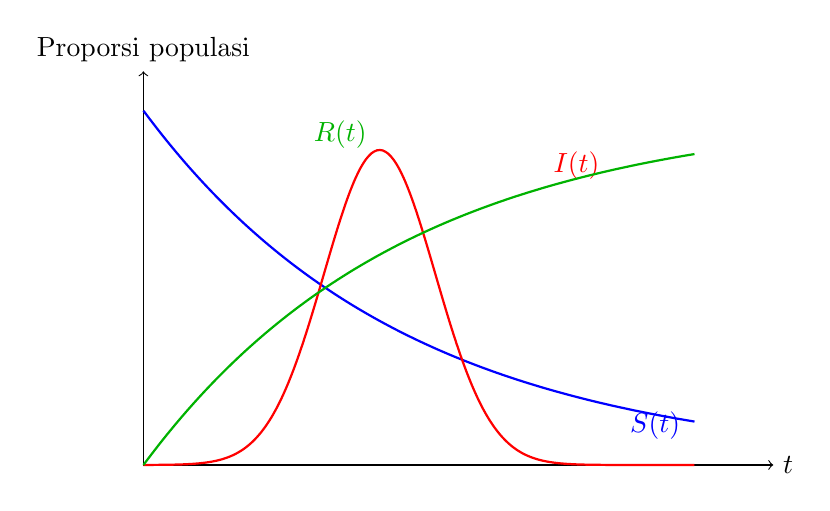
\begin{tikzpicture}
\draw[->] (0,0) -- (8,0) node[right] {$t$};
\draw[->] (0,0) -- (0,5) node[above] {Proporsi populasi};

% S(t)
\draw[smooth,domain=0:7,samples=100,variable=\x,blue,thick] 
  plot ({\x},{4.5*exp(-0.3*\x)});
\node[blue] at (6.5,0.5) {$S(t)$};

% I(t)
\draw[smooth,domain=0:7,samples=100,variable=\x,red,thick] 
  plot ({\x},{4*exp(-(\x-3)^2)});
\node[red] at (5.5,3.8) {$I(t)$};

% R(t)
\draw[smooth,domain=0:7,samples=100,variable=\x,green!70!black,thick] 
  plot ({\x},{4.5*(1-exp(-0.3*\x))});
\node[green!70!black] at (2.5,4.2) {$R(t)$};
\end{tikzpicture}
\end{center}

\subsection*{Interpretasi}
Dari grafik ini, pembaca dapat melihat:
\begin{itemize}
    \item $I(t)$ berbentuk lonceng: naik, mencapai puncak, lalu menurun.
    \item $S(t)$ selalu menurun, tidak pernah kembali naik.
    \item $R(t)$ terus meningkat, akhirnya mendekati total populasi $N$.
\end{itemize}
Polanya sangat sesuai dengan kenyataan wabah nyata: kasus harian meningkat, mencapai puncak, lalu menurun seiring semakin banyak individu yang memperoleh kekebalan.

\section{Keterbatasan Model Sederhana}

Meskipun model SIR dan variannya sangat berguna untuk memberikan wawasan kualitatif, kita harus ingat bahwa model ini dibangun di atas sejumlah asumsi yang kuat dan penyederhanaan yang signifikan. Beberapa keterbatasan utamanya antara lain:

\begin{itemize}
    \item {\jsg Populasi homogen.} Model mengasumsikan semua individu memiliki tingkat kontak yang sama. Pada kenyataannya, ada variasi besar: anak-anak, orang dewasa, dan lansia memiliki pola kontak yang berbeda.
    \item {\jsg Tidak ada struktur geografis.} Model klasik tidak mempertimbangkan perbedaan wilayah. Dalam kenyataan, wabah bisa terkonsentrasi di kota tertentu dan menyebar lebih lambat ke daerah lain.
    \item {\jsg Parameter konstan.} Laju penularan $\beta$ dan laju pemulihan $\gamma$ diasumsikan tetap. Padahal, intervensi seperti vaksinasi, lockdown, atau perubahan perilaku masyarakat dapat membuat parameter berubah seiring waktu.
    \item {\jsg Tidak ada kelahiran dan kematian alami.} Untuk jangka pendek, asumsi ini masuk akal, tetapi dalam jangka panjang, kelahiran dan kematian alami memengaruhi dinamika penyakit.
\end{itemize}

Keterbatasan ini menjelaskan mengapa model sederhana tidak dapat memprediksi secara akurat semua detail epidemi nyata. Namun, keindahannya justru terletak pada kesederhanaannya: dengan tiga persamaan sederhana, kita sudah bisa menjelaskan konsep inti epidemiologi.

\section{Latihan}

\begin{enumerate}
    \item Untuk parameter $\beta=0.2, \gamma=0.1$, dan $S(0)=500$, hitung nilai $R_0$. Apakah wabah akan menyebar atau padam?
    \item Simulasikan model SIR dengan $N=1000$, $S(0)=990$, $I(0)=10$, $R(0)=0$. Gambarkan kurva $S(t)$, $I(t)$, dan $R(t)$, lalu jelaskan dinamika yang terjadi.
    \item Modifikasi model SEIR untuk kasus penyakit dengan masa inkubasi rata-rata 5 hari (gunakan $\sigma = 1/5$). Bagaimana perbedaan perilaku $I(t)$ dibandingkan dengan model SIR?
    \item Diskusikan bagaimana vaksinasi dapat menurunkan nilai $R_0$ dan apa implikasinya terhadap konsep herd immunity.
\end{enumerate}

\section{Penutup}

Pada bab ini kita telah mempelajari {\jsg model epidemiologi kompartemen}: mulai dari SIR dasar, hingga varian SIS, SEIR, dan model dengan vaksinasi. Kita melihat bahwa model sederhana ini dapat menangkap fenomena inti wabah: pertumbuhan awal yang eksponensial, puncak kasus, dan meredanya epidemi. Kita juga memahami peran kunci bilangan reproduksi dasar $R_0$ dalam menentukan apakah wabah akan menyebar atau padam.

Meskipun penuh dengan asumsi, model ini tetap menjadi tonggak penting dalam epidemiologi matematika dan dasar bagi model yang lebih kompleks. Dari sinilah kemudian lahir model dengan struktur jaringan sosial, heterogenitas demografis, dan mobilitas spasial. Namun, sebagai batu loncatan pertama, model SIR dan variannya tetap relevan dan sangat instruktif.

Pada bab berikutnya, kita akan beralih dari epidemiologi ke bidang lain yang juga sarat dengan aplikasi pemodelan matematika, yaitu {\jsg model antrian (queueing models)}. Model ini banyak digunakan dalam studi sistem layanan kesehatan, transportasi, hingga jaringan komputer, di mana dinamika kedatangan dan pelayanan dapat dianalisis dengan kerangka matematika.

\vspace{2em}
\hrule
\vspace{1em}

%\subsection*{Transisi ke Bab Selanjutnya}

Setelah menelaah model epidemiologi, kita melihat bagaimana matematika dapat digunakan untuk memahami pergerakan penyakit dalam populasi. Dengan pendekatan kompartemen sederhana seperti SIR, SIS, dan SEIR, kita mampu menangkap fenomena kompleks seperti pertumbuhan awal yang eksponensial, tercapainya puncak kasus, hingga meredanya wabah. Bab ini sekaligus menunjukkan bahwa model matematika tidak hanya relevan di dunia ekologi atau biologi populasi, tetapi juga sangat penting dalam konteks kesehatan masyarakat.

Namun, dinamika yang melibatkan waktu dan interaksi individu tidak hanya muncul pada penyebaran penyakit. Dalam kehidupan sehari-hari, kita juga menemui situasi di mana {\jsg individu “datang” dan “menunggu” untuk dilayani}, baik itu pasien di rumah sakit, kendaraan di lampu lalu lintas, penumpang di bandara, atau bahkan paket data dalam jaringan komputer. Fenomena semacam ini menuntut pendekatan yang berbeda, yaitu dengan {\jsg model antrian (queueing models)}.

Pada bab berikutnya, kita akan mempelajari dasar-dasar teori antrian: bagaimana kedatangan pelanggan dimodelkan, bagaimana proses pelayanan berlangsung, serta bagaimana karakteristik sistem antrian dapat dianalisis. Sama seperti model epidemiologi yang memberi gambaran kuantitatif tentang penyakit, model antrian memberikan kerangka matematika untuk memahami efisiensi dan kinerja sistem layanan.

%=======================================================

\section*{Peta Konsep Model Antrian}

Teori antrian (\textit{queueing theory}) adalah cabang pemodelan matematika yang mempelajari bagaimana entitas—seperti manusia, kendaraan, atau paket data—datang ke suatu sistem untuk dilayani, lalu menunggu jika layanan sibuk, dan akhirnya meninggalkan sistem setelah selesai dilayani.

Struktur umum sistem antrian dapat digambarkan sebagai berikut:

\[
\text{Kedatangan} \;\longrightarrow\; \text{Antrian (waiting line)} \;\longrightarrow\; \text{Pelayanan (server)} \;\longrightarrow\; \text{Keluar}
\]

Untuk memahami teori antrian, ada beberapa komponen kunci:

\begin{enumerate}
    \item {\jsg Proses Kedatangan}  
    Bagaimana entitas masuk ke sistem.  
    - Bisa acak (misalnya distribusi Poisson).  
    - Bisa deterministik (misalnya setiap 10 detik datang satu mobil).
    
    \item {\jsg Distribusi Waktu Pelayanan}  
    Waktu yang dibutuhkan server untuk melayani satu entitas.  
    - Bisa eksponensial, normal, atau distribusi lain tergantung konteks.  
    
    \item {\jsg Jumlah Server}  
    Apakah layanan dilakukan oleh satu pelayan (single-server) atau banyak pelayan (multi-server).  
    
    \item {\jsg Aturan Disiplin Antrian}  
    Siapa yang dilayani lebih dulu?  
    - FIFO (First In First Out) → yang datang lebih dulu, dilayani lebih dulu.  
    - LIFO (Last In First Out).  
    - Prioritas (misalnya pasien gawat darurat).  
    
    \item {\jsg Kapasitas Sistem}  
    Apakah antrian dapat menampung jumlah tak terbatas, atau ada kapasitas terbatas (misalnya parkiran 50 mobil).  
    
    \item {\jsg Ukuran Kinerja}  
    Tujuan utama analisis adalah menghitung metrik kinerja, misalnya:  
    - Waktu rata-rata menunggu dalam antrian.  
    - Panjang rata-rata antrian.  
    - Utilisasi server (proporsi waktu server sibuk).  
    - Probabilitas sistem penuh (blocking probability).  
\end{enumerate}

\paragraph{Klasifikasi Model.}  
Model antrian sering ditulis dalam notasi Kendall: {\jsg $A/S/c$}, dengan:
\begin{itemize}
    \item $A$ = distribusi kedatangan (misalnya M = Markov/Poisson, D = deterministik).  
    \item $S$ = distribusi waktu pelayanan.  
    \item $c$ = jumlah server.  
\end{itemize}

Contoh:
- $M/M/1$: kedatangan Poisson, pelayanan eksponensial, satu server.  
- $M/M/c$: kedatangan Poisson, pelayanan eksponensial, $c$ server.  
- $M/D/1$: kedatangan Poisson, pelayanan deterministik, satu server.  

\paragraph{Aplikasi Nyata.}  
- Layanan kesehatan: pasien di ruang tunggu rumah sakit.  
- Transportasi: mobil menunggu lampu lalu lintas.  
- Telekomunikasi: paket data dalam jaringan internet.  
- Layanan publik: antrean di loket bank atau kantor pos.  

Peta konsep ini memberi kerangka berpikir: setiap sistem antrian dapat dipahami melalui kedatangan, antrian, pelayanan, dan ukuran kinerja.

\chapter{Model Antrian (Queueing Models)}

\section{Pendahuluan}

Setiap hari kita berhadapan dengan fenomena antrian. Di rumah sakit, pasien menunggu giliran konsultasi dengan dokter. Di jalan raya, kendaraan menumpuk di lampu lalu lintas. Di bank atau kantor pos, nasabah berdiri menunggu dilayani di loket. Bahkan di dunia digital, paket data yang melintas di jaringan komputer juga harus "mengantri" sebelum diproses oleh server. Semua fenomena tersebut memiliki pola yang sama: {\jsg ada kedatangan, ada antrian, ada pelayanan, lalu ada keberangkatan}.

Pertanyaan yang muncul kemudian adalah: dapatkah kita memprediksi seberapa panjang antrian akan terbentuk? Berapa lama rata-rata seseorang harus menunggu? Seberapa sibuk server atau pelayan bekerja? Pertanyaan-pertanyaan inilah yang dijawab oleh {\jsg teori antrian} (\textit{queueing theory}), suatu cabang matematika terapan yang berkembang pesat sejak awal abad ke-20.

Sejarah teori antrian dapat ditelusuri kembali pada penelitian Agner Krarup Erlang (1878–1929), seorang insinyur telekomunikasi asal Denmark. Erlang mempelajari bagaimana panggilan telepon masuk ke sentral telepon dan berapa banyak operator yang dibutuhkan agar panggilan tidak terlalu lama menunggu. Dari risetnya lahirlah model matematika pertama untuk antrian, yang hingga kini dikenal sebagai model Erlang.

\paragraph{Mengapa penting?}  
Teori antrian bukan hanya alat akademis, tetapi juga sangat praktis. Dengan model yang tepat, rumah sakit dapat mengatur jumlah dokter agar waktu tunggu pasien minimal. Operator transportasi dapat memperkirakan kepadatan lalu lintas. Perusahaan telekomunikasi dapat merancang jaringan agar tidak terjadi kemacetan data. Bahkan toko daring dapat memprediksi berapa banyak server yang dibutuhkan ketika menghadapi lonjakan transaksi pada hari-hari diskon besar.

\paragraph{Struktur Bab.}  
Pada bab ini, kita akan mempelajari:
\begin{enumerate}
    \item Komponen dasar sistem antrian: kedatangan, antrian, pelayanan, dan keberangkatan.
    \item Model antrian klasik $M/M/1$ (satu server dengan kedatangan Poisson dan pelayanan eksponensial).
    \item Perluasan ke model multi-server ($M/M/c$) dan variasi lain.
    \item Ukuran-ukuran kinerja sistem: panjang antrian rata-rata, waktu tunggu rata-rata, utilisasi server, dan probabilitas blocking.
    \item Contoh aplikasi nyata dalam layanan kesehatan, transportasi, dan jaringan komputer.
\end{enumerate}

Dengan mempelajari teori antrian, pembaca akan memperoleh alat baru untuk memahami dinamika “kemacetan” dalam berbagai sistem, baik fisik maupun digital, serta belajar bagaimana model matematika dapat membantu membuat keputusan yang lebih efisien.

\section{Komponen Dasar Sistem Antrian}

Setiap sistem antrian, sekompleks apa pun, dapat dipahami melalui empat komponen utama: {\jsg kedatangan}, {\jsg antrian}, {\jsg pelayanan}, dan {\jsg keberangkatan}. Dengan memahami masing-masing komponen, kita dapat membangun model matematika yang sesuai untuk menganalisis performa sistem.

\subsection{Kedatangan (Arrival Process)}

Kedatangan adalah bagaimana entitas (manusia, kendaraan, paket data, dan lain-lain) masuk ke dalam sistem. Dalam banyak kasus, kedatangan bersifat acak: kita tidak tahu persis kapan orang berikutnya akan datang. Untuk memodelkan fenomena ini, digunakan konsep probabilitas. Salah satu model kedatangan yang paling umum adalah {\jsg proses Poisson}, di mana jumlah kedatangan dalam suatu interval waktu mengikuti distribusi Poisson, dan jarak antar kedatangan mengikuti distribusi eksponensial.

Sebagai contoh, pasien yang datang ke unit gawat darurat rumah sakit atau mobil yang masuk ke gerbang tol dapat dimodelkan dengan proses Poisson. Namun, dalam beberapa situasi, kedatangan dapat bersifat deterministik, misalnya satu bus tiba setiap 15 menit secara teratur. Dengan demikian, pemilihan model kedatangan harus menyesuaikan dengan karakteristik sistem nyata.

\subsection{Antrian (Waiting Line)}

Jika semua server sibuk ketika entitas datang, entitas tersebut harus menunggu. Di sinilah antrian terbentuk. Panjang antrian dapat bersifat {\jsg tak terbatas} (misalnya antrean pasien di ruang tunggu) atau {\jsg terbatas} (misalnya antrean kendaraan di pom bensin dengan lahan parkir terbatas).

Aturan siapa yang dilayani terlebih dahulu disebut {\jsg disiplin antrian}. Beberapa disiplin umum adalah:
\begin{itemize}
    \item FIFO (First In First Out) — siapa datang lebih dulu, dilayani lebih dulu.
    \item LIFO (Last In First Out) — siapa datang terakhir, justru dilayani lebih dulu.
    \item Prioritas — entitas dengan kebutuhan lebih mendesak mendapat layanan lebih dulu (misalnya pasien gawat darurat).
\end{itemize}

\subsection{Pelayanan (Service Mechanism)}

Server adalah pihak atau mekanisme yang memberikan layanan. Jumlah server dapat bervariasi:
\begin{itemize}
    \item Sistem {\jsg single-server}, misalnya satu kasir di toko kecil.
    \item Sistem {\jsg multi-server}, misalnya beberapa loket di bank atau beberapa jalur tol otomatis.
\end{itemize}

Waktu pelayanan juga bisa acak. Dalam model klasik, waktu pelayanan sering diasumsikan mengikuti distribusi eksponensial. Namun, dalam kenyataan, bisa juga distribusi normal (jika waktu rata-rata relatif stabil) atau distribusi deterministik (misalnya mesin otomatis yang selalu butuh waktu sama untuk melayani satu pelanggan).

\subsection{Keberangkatan (Departure)}

Setelah selesai dilayani, entitas meninggalkan sistem. Dari sudut pandang pemodelan, keberangkatan ini menutup siklus antrian: entitas datang, menunggu, dilayani, lalu pergi. Analisis terhadap pola keberangkatan membantu kita memahami {\jsg output} dari sistem: berapa banyak entitas yang berhasil dilayani per satuan waktu, dan bagaimana kualitas layanan yang diterima.

\section{Notasi Kendall untuk Model Antrian}

Untuk mempermudah komunikasi dan klasifikasi, teori antrian menggunakan notasi baku yang diperkenalkan oleh David G. Kendall pada tahun 1953. Notasi ini menuliskan model antrian dalam bentuk:

\[
A/S/c
\]

dengan arti sebagai berikut:
\begin{itemize}
    \item $A$ = distribusi waktu kedatangan (arrival distribution).
    \item $S$ = distribusi waktu pelayanan (service time distribution).
    \item $c$ = jumlah server (servers).
\end{itemize}

\subsection{Distribusi Kedatangan ($A$)}

Huruf pertama menunjukkan pola kedatangan:
\begin{itemize}
    \item $M$ (\textit{Markovian}) berarti distribusi eksponensial atau proses Poisson.
    \item $D$ (\textit{Deterministic}) berarti waktu antar kedatangan selalu tetap.
    \item $G$ (\textit{General}) berarti distribusi umum, tanpa asumsi khusus.
\end{itemize}

\subsection{Distribusi Waktu Pelayanan ($S$)}

Huruf kedua menunjukkan distribusi waktu pelayanan. Notasi yang digunakan sama dengan pada kedatangan: $M$, $D$, atau $G$. Jadi, $M$ berarti waktu pelayanan eksponensial, $D$ berarti deterministik, dan $G$ berarti umum.

\subsection{Jumlah Server ($c$)}

Angka ketiga menunjukkan jumlah server. Misalnya:
\begin{itemize}
    \item $1$ berarti hanya ada satu pelayan.
    \item $c$ berarti ada $c$ pelayan paralel, semua melayani entitas dari satu antrian yang sama.
\end{itemize}

\subsection{Contoh Model Kendall}

\begin{itemize}
    \item $M/M/1$: kedatangan Poisson, pelayanan eksponensial, satu server. Ini adalah model paling klasik dan paling sering dipelajari.
    \item $M/M/c$: kedatangan Poisson, pelayanan eksponensial, $c$ server paralel.
    \item $M/D/1$: kedatangan Poisson, pelayanan deterministik, satu server.
    \item $D/M/1$: kedatangan deterministik, pelayanan eksponensial, satu server.
    \item $G/G/1$: model paling umum, baik kedatangan maupun pelayanan mengikuti distribusi bebas.
\end{itemize}

\paragraph{Interpretasi Praktis.}  
Misalnya, sebuah loket pembayaran tol otomatis dengan kedatangan mobil acak bisa dimodelkan sebagai $M/D/1$: kedatangan Poisson ($M$), pelayanan deterministik ($D$) karena waktu pembayaran relatif konstan, dan hanya ada satu jalur masuk ($1$). Sebaliknya, antrian pasien di poliklinik besar dengan banyak dokter dapat dimodelkan sebagai $M/M/c$.

\section{Model Klasik $M/M/1$}

Model $M/M/1$ adalah model antrian paling sederhana sekaligus paling fundamental. Ia menjadi titik awal hampir semua pengembangan teori antrian. Notasi $M/M/1$ berarti:
\begin{itemize}
    \item Kedatangan mengikuti proses Poisson ({\jsg Markovian}), dengan rata-rata $\lambda$ kedatangan per satuan waktu.
    \item Waktu pelayanan bersifat acak dengan distribusi eksponensial ({\jsg Markovian}), dengan rata-rata $\mu$ pelayanan per satuan waktu.
    \item Hanya ada satu server ({\jsg 1}).
\end{itemize}

\subsection{Asumsi Dasar}
Model $M/M/1$ dibangun di atas asumsi berikut:
\begin{enumerate}
    \item Kedatangan pelanggan bersifat independen dan mengikuti distribusi Poisson.
    \item Waktu pelayanan bersifat independen dan mengikuti distribusi eksponensial.
    \item Hanya ada satu antrian dan satu server.
    \item Disiplin antrian adalah FIFO (First In First Out).
    \item Kapasitas antrian tak terbatas (siapa pun yang datang akan mengantri jika server sibuk).
    \item Populasi sumber pelanggan dianggap sangat besar, sehingga laju kedatangan tidak tergantung pada jumlah orang yang sedang menunggu.
\end{enumerate}

\subsection{Utilisasi Sistem}
Konsep kunci dalam $M/M/1$ adalah {\jsg faktor utilisasi}, dilambangkan dengan $\rho$:
\[
\rho = \frac{\lambda}{\mu}.
\]

Artinya, $\rho$ adalah proporsi rata-rata waktu server sibuk. Jika $\rho < 1$, maka sistem stabil: rata-rata laju pelayanan lebih besar daripada rata-rata laju kedatangan, sehingga antrian tidak tumbuh tak terbatas. Jika $\rho \geq 1$, sistem tidak stabil: antrian akan bertambah panjang tanpa henti.

\subsection{Hasil Utama $M/M/1$}
Dengan analisis teori probabilitas (rantai Markov), dapat diturunkan hasil-hasil penting berikut:
\begin{itemize}
    \item Panjang rata-rata antrian (termasuk yang sedang dilayani):
    \[
    L = \frac{\rho}{1-\rho}.
    \]
    \item Waktu rata-rata yang dihabiskan pelanggan dalam sistem (menunggu + dilayani):
    \[
    W = \frac{1}{\mu - \lambda}.
    \]
    \item Panjang rata-rata antrian \textit{murni} (yang menunggu, tidak termasuk yang sedang dilayani):
    \[
    L_q = \frac{\rho^2}{1-\rho}.
    \]
    \item Waktu rata-rata menunggu dalam antrian:
    \[
    W_q = \frac{\rho}{\mu - \lambda}.
    \]
\end{itemize}

\subsection{Interpretasi}
Hasil-hasil di atas menunjukkan hubungan sederhana namun kuat:
\[
L = \lambda W, \qquad L_q = \lambda W_q,
\]
yang dikenal sebagai {\jsg Hukum Little} (\textit{Little’s Law}). Hukum ini berlaku sangat umum, tidak hanya untuk model $M/M/1$, dan menjadi dasar analisis sistem antrian modern.

\paragraph{Contoh.}  
Misalkan sebuah loket bank melayani rata-rata $\mu=20$ pelanggan per jam. Pelanggan datang rata-rata $\lambda=15$ per jam. Maka:
\[
\rho = \frac{15}{20} = 0.75.
\]
Artinya, server sibuk 75\% dari waktunya. Panjang antrian rata-rata adalah:
\[
L = \frac{0.75}{1-0.75} = 3.
\]
Sehingga rata-rata ada 3 orang dalam sistem (termasuk yang sedang dilayani). Waktu rata-rata yang dihabiskan pelanggan adalah:
\[
W = \frac{1}{20-15} = 0.2 \text{ jam} \approx 12 \text{ menit}.
\]
Dari sini manajer bank bisa menyimpulkan: rata-rata seorang pelanggan menunggu sekitar 12 menit sebelum selesai dilayani.

\section{Model Multi-Server $M/M/c$}

Dalam banyak situasi nyata, sebuah sistem tidak hanya memiliki satu pelayan, melainkan beberapa pelayan paralel. Misalnya, sebuah bank dengan beberapa loket, rumah sakit dengan beberapa dokter, atau bandara dengan banyak jalur pemeriksaan. Model ini digambarkan dengan notasi $M/M/c$, yang berarti:
\begin{itemize}
    \item Kedatangan mengikuti distribusi Poisson dengan rata-rata $\lambda$.
    \item Waktu pelayanan mengikuti distribusi eksponensial dengan rata-rata $\mu$ per server.
    \item Ada $c$ server paralel yang melayani dari satu antrian bersama.
\end{itemize}

\subsection{Asumsi Dasar}
\begin{enumerate}
    \item Kedatangan pelanggan acak dan independen (Poisson).
    \item Waktu pelayanan tiap server eksponensial dan independen.
    \item Semua server identik, dengan kecepatan pelayanan rata-rata $\mu$.
    \item Disiplin antrian adalah FIFO (First In First Out).
    \item Kapasitas antrian tidak terbatas.
\end{enumerate}

\subsection{Utilisasi Sistem}
Utilisasi rata-rata per server dalam sistem multi-server dihitung sebagai
\[
\rho = \frac{\lambda}{c\mu}.
\]
Jika $\rho < 1$, sistem stabil. Jika $\rho \geq 1$, sistem tidak stabil karena kedatangan lebih besar daripada kapasitas pelayanan total.

\subsection{Distribusi Steady-State}
Analisis $M/M/c$ lebih kompleks daripada $M/M/1$. Probabilitas $P_n$ bahwa terdapat $n$ pelanggan dalam sistem diturunkan dengan pendekatan rantai Markov. Hasil akhirnya dirangkum dalam bentuk {\jsg Erlang-C Formula}, yang menghitung probabilitas seorang pelanggan harus menunggu.

\subsection{Erlang-C Formula}
Probabilitas pelanggan harus menunggu dalam antrian adalah:
\[
P_\text{wait} = \dfrac{\frac{(c\rho)^c}{c!(1-\rho)}}{\sum_{n=0}^{c-1} \frac{(c\rho)^n}{n!} + \frac{(c\rho)^c}{c!(1-\rho)}}.
\]

Dari sini dapat dihitung:
\begin{itemize}
    \item Panjang antrian rata-rata:
    \[
    L_q = P_\text{wait} \cdot \frac{\rho}{1-\rho}.
    \]
    \item Waktu tunggu rata-rata dalam antrian:
    \[
    W_q = \frac{L_q}{\lambda}.
    \]
    \item Waktu total rata-rata dalam sistem:
    \[
    W = W_q + \frac{1}{\mu}.
    \]
    \item Jumlah rata-rata pelanggan dalam sistem:
    \[
    L = \lambda W.
    \]
\end{itemize}

\subsection{Contoh Numerik}
Misalkan sebuah call center memiliki $c=3$ operator. Rata-rata, $\lambda = 12$ panggilan masuk per jam, dan tiap operator mampu menangani $\mu = 5$ panggilan per jam. Maka:
\[
\rho = \frac{12}{3 \times 5} = 0.8.
\]
Artinya, setiap operator rata-rata sibuk 80\% dari waktunya.

Menggunakan formula Erlang-C, dapat dihitung bahwa probabilitas pelanggan harus menunggu adalah
\[
P_\text{wait} \approx 0.57.
\]
Panjang antrian rata-rata adalah
\[
L_q \approx 2.28,
\]
dan waktu tunggu rata-rata adalah
\[
W_q \approx 0.19 \text{ jam} \approx 11 \text{ menit}.
\]

\paragraph{Interpretasi.}  
Hasil ini menunjukkan bahwa meskipun ada tiga operator, lebih dari separuh pelanggan masih harus menunggu sebelum dilayani. Dengan menambah satu operator (menjadi $c=4$), utilisasi turun, probabilitas menunggu berkurang, dan kualitas layanan meningkat.

\section{Ukuran Kinerja Sistem Antrian}

Tujuan utama dari teori antrian bukan hanya menuliskan persamaan, tetapi juga memperoleh ukuran-ukuran yang dapat membantu pengambil keputusan. Dengan mengetahui panjang rata-rata antrian atau waktu tunggu rata-rata, manajer dapat menentukan apakah sistem bekerja dengan baik atau perlu ditingkatkan kapasitasnya. Berikut adalah ukuran-ukuran kinerja yang umum digunakan.

\subsection{Utilisasi Server ($\rho$)}

Utilisasi menunjukkan proporsi waktu server sibuk. Dalam model $M/M/1$, misalnya:
\[
\rho = \frac{\lambda}{\mu}.
\]
Jika $\rho$ terlalu kecil, berarti server sering menganggur (tidak efisien). Jika $\rho$ mendekati 1, server terlalu sibuk dan antrian menjadi panjang. Sistem yang seimbang biasanya memiliki $\rho$ antara 0.7 dan 0.9.

\subsection{Jumlah Rata-rata Pelanggan dalam Sistem ($L$)}

$L$ menyatakan rata-rata jumlah pelanggan dalam sistem, baik yang menunggu maupun yang sedang dilayani. Pada model $M/M/1$:
\[
L = \frac{\rho}{1-\rho}.
\]

\subsection{Jumlah Rata-rata Pelanggan dalam Antrian ($L_q$)}

$L_q$ hanya menghitung pelanggan yang \textit{menunggu}, tidak termasuk yang sedang dilayani. Pada $M/M/1$:
\[
L_q = \frac{\rho^2}{1-\rho}.
\]

\subsection{Waktu Rata-rata dalam Sistem ($W$)}

$W$ adalah waktu rata-rata yang dihabiskan pelanggan sejak masuk hingga keluar dari sistem (menunggu + dilayani). Pada $M/M/1$:
\[
W = \frac{1}{\mu - \lambda}.
\]

\subsection{Waktu Rata-rata Menunggu ($W_q$)}

$W_q$ adalah waktu rata-rata yang dihabiskan pelanggan hanya untuk menunggu dalam antrian. Pada $M/M/1$:
\[
W_q = \frac{\rho}{\mu - \lambda}.
\]

\subsection{Probabilitas Menunggu ($P_\text{wait}$)}

Pada sistem multi-server ($M/M/c$), penting untuk menghitung peluang bahwa pelanggan baru yang datang harus menunggu sebelum dilayani. Probabilitas ini dirumuskan dengan {\jsg Erlang-C formula}, yang telah dijelaskan sebelumnya. Nilai $P_\text{wait}$ menjadi indikator kualitas layanan.

\subsection{Hukum Little}

Ukuran-ukuran ini saling berkaitan melalui hukum fundamental dalam teori antrian, yaitu {\jsg Hukum Little}:
\[
L = \lambda W, \qquad L_q = \lambda W_q.
\]

Hukum ini berlaku sangat umum, tidak bergantung pada distribusi tertentu, asalkan sistem stabil. Intinya, jumlah rata-rata pelanggan dalam sistem sama dengan laju kedatangan dikali waktu rata-rata yang dihabiskan pelanggan.

\paragraph{Interpretasi Praktis.}  
Misalnya, jika rata-rata ada 10 pelanggan dalam sistem ($L=10$) dan laju kedatangan adalah 5 pelanggan per menit ($\lambda=5$), maka hukum Little menjamin waktu rata-rata dalam sistem adalah:
\[
W = \frac{L}{\lambda} = \frac{10}{5} = 2 \text{ menit}.
\]

\paragraph{Kesimpulan.}  
Dengan ukuran-ukuran ini, kita bisa mengevaluasi performa sistem secara kuantitatif: berapa lama orang menunggu, berapa banyak yang menumpuk, dan seberapa sibuk server. Dari sini, keputusan manajerial dapat dibuat, misalnya apakah perlu menambah server, mengubah aturan antrian, atau mengendalikan laju kedatangan.

\section{Aplikasi Nyata Model Antrian}

Teori antrian bukan hanya konstruksi matematis abstrak, tetapi juga memiliki aplikasi luas dalam berbagai bidang kehidupan sehari-hari. Dengan memahami model antrian, kita dapat merancang sistem layanan yang lebih efisien, mengurangi waktu tunggu, dan meningkatkan kepuasan pengguna. Berikut adalah beberapa contoh aplikasinya.

\subsection{Rumah Sakit dan Layanan Kesehatan}

Di ruang tunggu rumah sakit atau klinik, pasien datang secara acak dan dilayani oleh sejumlah dokter atau tenaga medis. Jika pasien datang lebih cepat daripada kemampuan dokter melayani, maka antrian terbentuk. Model $M/M/c$ dapat digunakan untuk memperkirakan:
\begin{itemize}
    \item Rata-rata waktu tunggu pasien.
    \item Jumlah dokter yang optimal agar pasien tidak menunggu terlalu lama.
    \item Utilisasi dokter (berapa persen waktu mereka sibuk).
\end{itemize}

Sebagai contoh, dalam unit gawat darurat, manajemen rumah sakit dapat menghitung berapa banyak dokter yang harus bertugas pada jam sibuk agar pasien gawat tidak menunggu terlalu lama, sambil memastikan sumber daya tidak berlebih pada jam sepi.

\subsection{Transportasi dan Lalu Lintas}

Antrian sering muncul di dunia transportasi: kendaraan menunggu di lampu lalu lintas, kapal menunggu giliran di pelabuhan, atau pesawat menunggu antrean lepas landas di bandara. Dengan model antrian, operator dapat:
\begin{itemize}
    \item Memperkirakan panjang antrian rata-rata pada jam sibuk.
    \item Menentukan waktu hijau lampu lalu lintas yang optimal.
    \item Menghitung kapasitas dermaga atau landasan pacu yang dibutuhkan.
\end{itemize}

Sebagai ilustrasi, lampu lalu lintas di persimpangan padat dapat dimodelkan dengan sistem antrian periodik: kendaraan datang mengikuti distribusi tertentu, lalu menunggu hingga lampu hijau menyala (server “aktif”). Analisis ini membantu perencanaan lalu lintas perkotaan.

\subsection{Telekomunikasi dan Jaringan Komputer}

Di era digital, antrian tidak hanya berupa orang atau kendaraan, tetapi juga {\jsg data}. Paket data yang melewati router internet, pesan yang masuk ke server email, atau transaksi di platform e-commerce semuanya tunduk pada dinamika antrian. Model $M/M/1$ dan $M/M/c$ banyak digunakan untuk:
\begin{itemize}
    \item Menentukan kapasitas buffer router.
    \item Memperkirakan waktu delay rata-rata dalam jaringan.
    \item Merancang server agar mampu menangani lonjakan lalu lintas (traffic surge).
\end{itemize}

Sebagai contoh, ketika sebuah toko daring mengadakan diskon besar, ribuan transaksi dapat masuk secara bersamaan. Dengan teori antrian, perusahaan dapat menghitung berapa banyak server yang dibutuhkan agar sistem tidak macet.

\subsection{Layanan Publik dan Industri}

Di kantor pos, bank, restoran cepat saji, atau bahkan wahana rekreasi, antrian adalah bagian tak terpisahkan dari pengalaman pelanggan. Model antrian membantu menjawab pertanyaan praktis:
\begin{itemize}
    \item Apakah perlu menambah loket atau kasir pada jam sibuk?
    \item Berapa lama rata-rata pelanggan akan menunggu?
    \item Bagaimana mendesain jalur antrian agar lebih efisien?
\end{itemize}

Sebagai contoh, manajemen bank dapat memutuskan apakah lebih baik memiliki satu antrian panjang untuk beberapa loket (satu antrian $M/M/c$), atau beberapa antrian terpisah (beberapa $M/M/1$). Analisis matematis dapat menunjukkan opsi mana yang lebih efisien dalam mengurangi waktu tunggu.

\section{Latihan}

\begin{enumerate}
    \item Sebuah loket tiket bioskop menerima pelanggan dengan laju rata-rata $\lambda = 10$ orang per jam. Waktu pelayanan rata-rata $\mu = 12$ orang per jam.  
    \begin{enumerate}
        \item Hitung faktor utilisasi $\rho$.  
        \item Tentukan waktu tunggu rata-rata dalam sistem ($W$) dan panjang antrian rata-rata ($L$).  
    \end{enumerate}

    \item Sebuah call center memiliki 4 operator ($c=4$). Kedatangan pelanggan mengikuti distribusi Poisson dengan rata-rata $\lambda = 40$ panggilan per jam, dan tiap operator mampu melayani rata-rata $\mu = 15$ panggilan per jam.  
    \begin{enumerate}
        \item Hitung utilisasi per operator.  
        \item Gunakan formula Erlang-C untuk memperkirakan probabilitas pelanggan harus menunggu ($P_{\text{wait}}$).  
        \item Hitung panjang antrian rata-rata ($L_q$).  
    \end{enumerate}

    \item Sebuah sistem komputer menangani paket data yang datang dengan laju $\lambda = 200$ paket per detik. Waktu pelayanan rata-rata adalah $1/\mu = 0.004$ detik.  
    \begin{enumerate}
        \item Apakah sistem stabil?  
        \item Hitung waktu tunggu rata-rata dalam antrian ($W_q$).  
    \end{enumerate}

    \item Diskusikan: dalam konteks layanan publik (bank, rumah sakit, restoran), manakah yang lebih efisien — satu antrian panjang dengan banyak server ($M/M/c$), atau beberapa antrian paralel dengan masing-masing server sendiri ($c$ buah $M/M/1$)?
\end{enumerate}

\section{Penutup}

Pada bab ini, kita mempelajari {\jsg teori antrian}, mulai dari konsep dasar hingga model matematis klasik. Kita memahami bahwa setiap sistem antrian dapat dianalisis melalui empat komponen: kedatangan, antrian, pelayanan, dan keberangkatan. Dengan menggunakan notasi Kendall, kita mengenal berbagai model standar seperti $M/M/1$ dan $M/M/c$, yang menjadi tulang punggung teori antrian.

Hasil-hasil penting, seperti panjang antrian rata-rata, waktu tunggu rata-rata, dan utilisasi server, memberikan wawasan kuantitatif yang sangat berguna. Kita juga melihat bahwa hukum Little ($L = \lambda W$) berlaku sangat umum dan menjadi prinsip dasar dalam analisis sistem antrian.

Aplikasi teori antrian sangat luas: dari rumah sakit dan transportasi hingga jaringan komputer dan layanan publik. Dengan model yang tepat, kita dapat merancang sistem yang lebih efisien, mengurangi waktu tunggu, dan meningkatkan kualitas layanan.

Bab berikutnya akan memperluas horizon kita dengan membahas {\jsg model stokastik lain yang terkait dengan proses Markov}, yang menjadi dasar lebih banyak aplikasi dalam bidang keuangan, biologi, dan ilmu komputer. Dengan demikian, pembaca dapat melihat keterhubungan antara antrian, epidemiologi, dan banyak fenomena stokastik lain di dunia nyata.

\subsection*{Transisi ke Bab Selanjutnya}

Melalui pembahasan teori antrian, kita telah melihat bagaimana matematika mampu menjelaskan fenomena \textit{kemacetan layanan}: bagaimana entitas datang, menunggu, dilayani, lalu keluar dari sistem. Dengan formulasi probabilistik sederhana, kita bisa memperkirakan panjang antrian, waktu tunggu, hingga utilisasi server. Semua itu didasarkan pada ide bahwa kedatangan dan pelayanan bersifat acak, sehingga analisis antrian tidak bisa dilepaskan dari konsep probabilitas dan proses stokastik.

Hal ini membawa kita pada pertanyaan yang lebih mendasar: {\jsg bagaimana cara memodelkan dinamika acak (stokastik) secara umum?} Kedatangan pelanggan yang mengikuti distribusi Poisson, waktu pelayanan yang eksponensial, maupun perpindahan antarstatus dalam epidemiologi—semuanya dapat dipandang sebagai contoh dari suatu {\jsg proses Markov}, yaitu sistem stokastik yang berevolusi dari waktu ke waktu berdasarkan aturan probabilitas tertentu.

Oleh karena itu, pada bab berikutnya kita akan mempelajari {\jsg model stokastik berbasis proses Markov}. Bab ini akan memperkenalkan definisi formal rantai Markov, sifat-sifat utamanya, serta contoh aplikasinya dalam berbagai bidang—mulai dari biologi, keuangan, hingga ilmu komputer. Dengan pemahaman ini, pembaca akan memiliki fondasi yang lebih kokoh untuk menganalisis fenomena stokastik yang kompleks.

%=======================================================

\chapter{Model Stokastik dan Rantai Markov}

\section{Pendahuluan}

Dalam bab-bab sebelumnya kita telah banyak membahas model yang bersifat deterministik, seperti pertumbuhan populasi eksponensial dan logistik, interaksi predator–prey Lotka–Volterra, serta model epidemiologi SIR. Kita juga mengenal model semi-stokastik dalam teori antrian, di mana kedatangan dan pelayanan dimodelkan dengan distribusi probabilitas tertentu. Semua contoh itu menunjukkan satu hal: {\jsg fenomena dunia nyata sering kali dipengaruhi oleh unsur ketidakpastian (stokastisitas)}.

Tidak semua hal bisa diprediksi secara tepat. Jumlah kelahiran dan kematian setiap hari, waktu kedatangan pasien di rumah sakit, lamanya seseorang sakit flu, atau bahkan harga saham di bursa—semuanya mengandung komponen acak. Karena itu, untuk melangkah lebih jauh kita perlu membekali diri dengan kerangka matematika yang secara khusus didesain untuk menganalisis {\jsg dynamika acak}, yaitu {\jsg proses stokastik}.

\paragraph{Mengapa penting?}  
Proses stokastik menyediakan alat bagi kita untuk memodelkan fenomena yang tidak dapat dijelaskan dengan persamaan deterministik. Alih-alih memberi prediksi pasti, model stokastik memberikan distribusi kemungkinan: seberapa besar peluang suatu keadaan terjadi, berapa lama rata-rata sistem berada pada kondisi tertentu, atau bagaimana kemungkinan sistem berpindah dari satu keadaan ke keadaan lain.

\paragraph{Contoh sehari-hari.}
\begin{itemize}
    \item {\jsg Biologi:} Jumlah molekul dalam suatu reaksi kimia di dalam sel berfluktuasi secara acak akibat benturan antarpartikel.
    \item {\jsg Kesehatan:} Waktu kedatangan pasien di unit gawat darurat tidak dapat diprediksi dengan pasti, tetapi dapat dimodelkan dengan distribusi probabilitas.
    \item {\jsg Ekonomi:} Harga saham tidak mengikuti pola deterministik, melainkan bergerak secara stokastik dengan fluktuasi acak dari menit ke menit.
    \item {\jsg Informatika:} Paket data dalam jaringan komputer bergerak melewati router dengan waktu tunggu yang acak, sehingga analisis kinerja jaringan memerlukan model stokastik.
\end{itemize}

\paragraph{Sejarah singkat.}  
Konsep formal proses stokastik diperkenalkan oleh Andrey Andreyevich Markov (1856–1922), seorang matematikawan Rusia. Ia mempelajari rantai karakter huruf dalam teks literatur dan memperlihatkan bahwa probabilitas suatu huruf muncul bergantung hanya pada huruf sebelumnya. Dari sinilah lahir gagasan tentang {\jsg rantai Markov}, yang kemudian berkembang menjadi salah satu kerangka terpenting dalam analisis sistem stokastik modern.

\paragraph{Struktur Bab.}  
Pada bab ini kita akan mempelajari:
\begin{enumerate}
    \item Definisi formal proses stokastik dan rantai Markov.
    \item Sifat-sifat dasar rantai Markov (transisi, distribusi stasioner, klasifikasi keadaan).
    \item Contoh aplikasi Markov dalam biologi, epidemiologi, ekonomi, dan ilmu komputer.
    \item Perluasan ke proses Markov kontinu waktu.
\end{enumerate}

Dengan fondasi ini, pembaca akan memahami bagaimana memodelkan sistem yang mengandung unsur acak, serta bagaimana membuat prediksi probabilistik yang dapat diuji secara kuantitatif.

\section{Definisi Formal: Proses Stokastik dan Rantai Markov}

\subsection{Proses Stokastik}

Sebuah {\jsg proses stokastik} adalah sebuah keluarga variabel acak $\{X(t), t \in T\}$ yang diindeks oleh waktu $t$.  
\begin{itemize}
    \item $T$ bisa berupa himpunan diskrit ($t=0,1,2,\dots$) atau kontinu ($t \geq 0$).  
    \item $X(t)$ menyatakan keadaan sistem pada waktu $t$.  
\end{itemize}

Dengan kata lain, proses stokastik adalah model matematis untuk sistem yang berkembang secara acak seiring waktu.

\paragraph{Contoh:}
\begin{enumerate}
    \item Jumlah pelanggan di bank pada waktu $t$ tertentu.  
    \item Status cuaca harian (cerah, mendung, hujan).  
    \item Harga saham suatu perusahaan setiap jam.  
\end{enumerate}

\subsection{Rantai Markov Diskrit}

Sebuah {\jsg rantai Markov} adalah proses stokastik dengan {\jsg properti Markov}: keadaan pada waktu berikutnya hanya bergantung pada keadaan saat ini, bukan pada masa lalu yang lebih jauh. Secara matematis:

\[
P\{X_{n+1} = j \;|\; X_n = i, X_{n-1}, \dots, X_0\} = P\{X_{n+1} = j \;|\; X_n = i\}.
\]

Artinya, masa depan hanya bergantung pada kondisi saat ini. Inilah yang disebut sifat “memori pendek” (memoryless).

\subsection{Probabilitas Transisi}

Probabilitas perpindahan dari keadaan $i$ ke keadaan $j$ dalam satu langkah ditulis:
\[
p_{ij} = P\{X_{n+1}=j \,|\, X_n=i\}.
\]

Semua probabilitas transisi ini dapat disusun dalam sebuah {\jsg matriks transisi}:
\[
P = 
\begin{bmatrix}
p_{11} & p_{12} & \cdots & p_{1m} \\
p_{21} & p_{22} & \cdots & p_{2m} \\
\vdots & \vdots & \ddots & \vdots \\
p_{m1} & p_{m2} & \cdots & p_{mm} \\
\end{bmatrix},
\]
dengan syarat:
\[
p_{ij} \geq 0, \qquad \sum_{j} p_{ij} = 1.
\]

\subsection{Contoh Sederhana: Cuaca}

Misalkan cuaca hanya punya dua keadaan: cerah (C) dan hujan (H). Probabilitas transisi:
\[
P = 
\begin{bmatrix}
0.7 & 0.3 \\
0.4 & 0.6
\end{bmatrix}.
\]

Interpretasi:
\begin{itemize}
    \item Jika hari ini cerah, peluang besok cerah lagi adalah 0.7, peluang hujan 0.3.
    \item Jika hari ini hujan, peluang besok tetap hujan 0.6, peluang cerah 0.4.
\end{itemize}

Dengan model ini, kita bisa menghitung probabilitas cuaca dalam beberapa hari ke depan dengan mengalikan matriks transisi secara berulang.

\section{Distribusi Probabilitas dan Evolusi Sistem}

\subsection{Distribusi Keadaan}

Pada awal waktu $n=0$, sistem memiliki {\jsg distribusi awal} yang dituliskan dalam bentuk vektor baris:
\[
\pi^{(0)} = [ \pi_1^{(0)}, \pi_2^{(0)}, \dots, \pi_m^{(0)} ],
\]
dengan $\pi_i^{(0)} = P\{X_0 = i\}$ dan $\sum_{i=1}^m \pi_i^{(0)} = 1$.

Distribusi ini menyatakan probabilitas sistem berada di setiap keadaan pada waktu awal.

\subsection{Evolusi dengan Matriks Transisi}

Jika $P$ adalah matriks transisi, maka distribusi keadaan pada langkah ke-$n$ dapat dihitung dengan:
\[
\pi^{(n)} = \pi^{(0)} P^n.
\]

Artinya, untuk mengetahui peluang sistem berada di setiap keadaan setelah $n$ langkah, kita cukup mengalikan distribusi awal dengan pangkat ke-$n$ dari matriks transisi.

\subsection{Contoh: Model Cuaca}

Kita gunakan matriks transisi cuaca dua keadaan:
\[
P =
\begin{bmatrix}
0.7 & 0.3 \\
0.4 & 0.6
\end{bmatrix}.
\]

Misalkan hari ini (waktu $n=0$) pasti cerah. Distribusi awal:
\[
\pi^{(0)} = [1, \; 0].
\]

\paragraph{Probabilitas besok ($n=1$):}
\[
\pi^{(1)} = \pi^{(0)} P = [1,0] 
\begin{bmatrix}
0.7 & 0.3 \\
0.4 & 0.6
\end{bmatrix}
= [0.7, \; 0.3].
\]
Artinya, besok ada peluang 70\% cerah, 30\% hujan.

\paragraph{Probabilitas lusa ($n=2$):}
\[
\pi^{(2)} = \pi^{(1)} P = [0.7, 0.3] 
\begin{bmatrix}
0.7 & 0.3 \\
0.4 & 0.6
\end{bmatrix}
= [0.61, \; 0.39].
\]
Jadi dalam dua hari, peluang cerah adalah 61\%, hujan 39\%.

\subsection{Interpretasi}

Dengan cara ini, rantai Markov memungkinkan kita memproyeksikan perilaku sistem dalam jangka pendek maupun panjang. Semakin jauh ke depan ($n$ besar), distribusi $\pi^{(n)}$ dapat mendekati {\jsg distribusi stasioner}, yang akan kita bahas pada bagian berikutnya.

\section{Distribusi Stasioner dan Sifat Jangka Panjang}

\subsection{Definisi Distribusi Stasioner}

Sebuah vektor probabilitas $\pi = [\pi_1, \pi_2, \dots, \pi_m]$ disebut {\jsg distribusi stasioner} dari rantai Markov dengan matriks transisi $P$ jika memenuhi:
\[
\pi = \pi P, \qquad \sum_{i=1}^m \pi_i = 1, \quad \pi_i \geq 0.
\]

Artinya, jika sistem memulai dengan distribusi $\pi$, maka pada setiap langkah berikutnya distribusi itu tidak berubah. Distribusi stasioner menggambarkan keadaan jangka panjang dari sistem.

\subsection{Interpretasi}

Distribusi stasioner bisa dipandang sebagai “proporsi waktu” yang dihabiskan sistem dalam setiap keadaan ketika $n \to \infty$. Misalnya, jika $\pi = [0.75, 0.25]$, artinya dalam jangka panjang sistem akan berada dalam keadaan 1 selama 75\% waktu, dan dalam keadaan 2 selama 25\% waktu.

\subsection{Contoh: Model Cuaca}

Kembali ke matriks transisi cuaca:
\[
P =
\begin{bmatrix}
0.7 & 0.3 \\
0.4 & 0.6
\end{bmatrix}.
\]

Distribusi stasioner $\pi = [\pi_C, \pi_H]$ harus memenuhi:
\[
\pi = \pi P.
\]

Sehingga:
\[
\pi_C = 0.7 \pi_C + 0.4 \pi_H, \qquad
\pi_H = 0.3 \pi_C + 0.6 \pi_H.
\]

Ditambah syarat normalisasi $\pi_C + \pi_H = 1$. Dari persamaan pertama:
\[
\pi_C = 0.7\pi_C + 0.4(1-\pi_C),
\]
\[
\pi_C = 0.7\pi_C + 0.4 - 0.4\pi_C,
\]
\[
\pi_C - 0.3\pi_C = 0.4,
\]
\[
0.7\pi_C = 0.4 \quad \Rightarrow \quad \pi_C = \frac{4}{7}.
\]
Maka:
\[
\pi_H = 1 - \pi_C = \frac{3}{7}.
\]

\paragraph{Interpretasi.}  
Dalam jangka panjang, sistem cuaca ini akan cerah sekitar 57\% waktu, dan hujan sekitar 43\% waktu, tidak peduli bagaimana kondisi awalnya.

\subsection{Syarat Eksistensi}

Tidak semua rantai Markov memiliki distribusi stasioner unik. Agar distribusi stasioner eksis dan unik, rantai harus memenuhi kondisi:
\begin{itemize}
    \item {\jsg Irreducible:} semua keadaan saling terhubung (setiap keadaan dapat dicapai dari keadaan lain dalam sejumlah langkah).
    \item {\jsg Aperiodik:} sistem tidak terjebak dalam siklus periodik yang kaku.
\end{itemize}

Jika kedua syarat ini terpenuhi, rantai Markov bersifat {\jsg ergodik}, dan distribusi $\pi$ yang unik akan menggambarkan perilaku jangka panjang sistem.


%=======================================================
\chapter{Rantai Markov (Markov Chains)}

\section{Pendahuluan}
Banyak fenomena dalam dunia nyata bersifat stokastik: hasilnya tidak pasti, melainkan dipengaruhi oleh peluang. Salah satu kerangka matematis yang sederhana namun kuat untuk mempelajari fenomena stokastik adalah {\jsg rantai Markov} (Markov chain). 

Konsep ini pertama kali diperkenalkan oleh matematikawan Rusia, Andrey A. Markov (1856–1922), untuk menganalisis ketergantungan antar huruf dalam teks puisi. Sejak saat itu, rantai Markov digunakan luas dalam ilmu komputer, ekonomi, biologi, dan rekayasa.

\section{Definisi Rantai Markov}
Sebuah proses stokastik $\{X_n, n=0,1,2,\dots\}$ disebut {\jsg rantai Markov} jika memenuhi sifat {\jsg Markov}:
\[
P(X_{n+1} = j \mid X_n = i, X_{n-1},\dots,X_0) = P(X_{n+1} = j \mid X_n = i).
\]

Artinya, peluang kondisi berikutnya hanya bergantung pada kondisi saat ini, bukan pada sejarah sebelumnya. 

\section{Matriks Transisi}
Rantai Markov didefinisikan oleh {\jsg matriks transisi} $P = (p_{ij})$:
\[
p_{ij} = P(X_{n+1}=j \mid X_n = i).
\]

Sifat matriks transisi:
\begin{itemize}
    \item $0 \leq p_{ij} \leq 1$.
    \item $\sum_j p_{ij} = 1$ untuk setiap $i$.
\end{itemize}

Contoh (model cuaca sederhana):
\[
P = \begin{bmatrix}
0.7 & 0.3 \\
0.4 & 0.6
\end{bmatrix},
\]
dengan state: 1 = cerah, 2 = hujan. Artinya, jika hari ini cerah, besok cerah lagi dengan peluang 0.7, dan hujan dengan peluang 0.3.

\section{Distribusi Keadaan}
Jika distribusi awal adalah $\pi^{(0)} = [\pi_1^{(0)}, \pi_2^{(0)}, \dots]$, maka distribusi pada langkah ke-$n$ adalah:
\[
\pi^{(n)} = \pi^{(0)} P^n.
\]

\section{Klasifikasi State}
\begin{itemize}
    \item {\jsg State recurrent}: proses akan kembali ke state tersebut dengan probabilitas 1.
    \item {\jsg State transient}: ada probabilitas positif proses tidak pernah kembali.
    \item {\jsg State absorbing}: $p_{ii}=1$, artinya jika masuk ke state ini, proses tidak pernah keluar.
\end{itemize}

\section{Teorema Limit}
Jika rantai Markov irreducible dan aperiodik, maka ada distribusi stasioner $\pi$ sehingga:
\[
\pi = \pi P, \quad \sum_i \pi_i = 1.
\]

Distribusi stasioner menggambarkan proporsi jangka panjang waktu yang dihabiskan dalam setiap state.

\section{Contoh Aplikasi}
\subsection{Model Cuaca}
Misalkan cuaca hanya dua kemungkinan: cerah (C) dan hujan (H), dengan matriks transisi:
\[
P = \begin{bmatrix}
0.8 & 0.2 \\
0.5 & 0.5
\end{bmatrix}.
\]

Jika hari ini cerah, maka peluang dua hari kemudian juga cerah:
\[
P(X_2=C \mid X_0=C) = (P^2)_{CC}.
\]

\subsection{Permainan Judi}
Dalam permainan sederhana, seorang pemain memiliki modal $i$. Setiap putaran, modal bertambah 1 dengan peluang $p$ atau berkurang 1 dengan peluang $q=1-p$. State $0$ dan $N$ adalah absorbing (kebangkrutan atau kemenangan). Rantai Markov digunakan untuk menghitung probabilitas kebangkrutan.

\subsection{Produksi Mesin}
Mesin bisa dalam kondisi baik (B) atau rusak (R). Peluang transisi: mesin baik tetap baik 0.9, rusak menjadi baik 0.6. Dengan Markov chain, kita dapat menghitung proporsi waktu mesin dalam kondisi rusak.

\section{Contoh Numerik}
Misalkan $P = \begin{bmatrix} 0.7 & 0.3 \\ 0.4 & 0.6 \end{bmatrix}$, distribusi awal $\pi^{(0)} = [1,0]$.

\begin{itemize}
    \item $\pi^{(1)} = [0.7, 0.3]$.
    \item $\pi^{(2)} = \pi^{(0)} P^2 = [0.67, 0.33]$.
    \item Dalam jangka panjang, distribusi stasioner $\pi = [0.571, 0.429]$.
\end{itemize}

Interpretasi: dalam jangka panjang, sekitar 57.1\% hari cerah, 42.9\% hujan.

\section{Latihan}
\begin{enumerate}
    \item Sebuah rantai Markov dengan state $\{1,2,3\}$ memiliki matriks transisi:
    \[
    P = \begin{bmatrix}
    0.5 & 0.5 & 0 \\
    0.2 & 0.6 & 0.2 \\
    0 & 0.4 & 0.6
    \end{bmatrix}.
    \]
    Tentukan distribusi stasionernya.
    \item Dalam model permainan judi dengan $p=0.4$, $q=0.6$, hitung probabilitas kebangkrutan jika modal awal $i=3$ dan modal target $N=5$.
    \item Diskusikan aplikasi rantai Markov dalam \textit{PageRank} (algoritma mesin pencari).
\end{enumerate}

\section{Penutup}
Bab ini memperkenalkan dasar-dasar rantai Markov: definisi, matriks transisi, klasifikasi state, distribusi stasioner, dan contoh aplikasinya. Konsep ini menjadi pondasi untuk model stokastik yang lebih kompleks, seperti teori antrian, simulasi Monte Carlo, dan proses stokastik kontinu. Pada bab berikutnya, kita akan mempelajari {\jsg model Input–Output Leontief dalam Ekonomi}, yang merupakan contoh model aljabar linier dalam pemodelan sistem.



%=======================================================
\chapter{Model Input–Output Leontief dalam Ekonomi}

\section{Pendahuluan}
Dalam sebuah perekonomian, berbagai sektor saling bergantung. Misalnya, sektor pertanian membutuhkan pupuk (industri kimia), transportasi, dan energi; sementara sektor industri makanan membutuhkan hasil pertanian. Pertanyaan penting adalah: bagaimana perubahan permintaan pada satu sektor memengaruhi produksi sektor lain?

Wassily Leontief (1906–1999), ekonom peraih Nobel 1973, memperkenalkan {\jsg model input–output} yang memformulasikan keterkaitan antar-sektor dalam bentuk aljabar linier. Model ini masih digunakan hingga kini dalam perencanaan ekonomi, analisis kebijakan, dan perhitungan dampak multiplikasi sektor.

\section{Formulasi Dasar}
Misalkan ada $n$ sektor dalam perekonomian. Definisikan:
\begin{itemize}
    \item $x_i$: total output sektor $i$.
    \item $z_{ij}$: output sektor $i$ yang digunakan sektor $j$.
    \item $f_i$: permintaan akhir (\textit{final demand}) terhadap sektor $i$.
\end{itemize}

Neraca untuk sektor $j$:
\[
x_j = \sum_{i=1}^n z_{ij} + f_j.
\]

\subsection{Koefisien Input}
Definisikan koefisien input $a_{ij}$:
\[
a_{ij} = \frac{z_{ij}}{x_j},
\]
yang menunjukkan berapa banyak input dari sektor $i$ dibutuhkan untuk menghasilkan satu unit output sektor $j$.

Dengan demikian, sistem dapat ditulis:
\[
x_j = \sum_{i=1}^n a_{ij} x_j + f_j.
\]

\section{Bentuk Matriks}
Definisikan:
\begin{itemize}
    \item $x = (x_1, x_2, \dots, x_n)^T$ = vektor output.
    \item $f = (f_1, f_2, \dots, f_n)^T$ = vektor permintaan akhir.
    \item $A = (a_{ij})$ = matriks koefisien input.
\end{itemize}

Model Leontief terbuka ditulis:
\[
x = Ax + f.
\]

Sehingga:
\[
(I - A)x = f, \quad \Rightarrow \quad x = (I-A)^{-1} f.
\]

Matriks $(I-A)^{-1}$ disebut {\jsg Leontief inverse}, menggambarkan total dampak (langsung dan tidak langsung) perubahan permintaan akhir terhadap output sektor.

\section{Model Tertutup dan Terbuka}
\begin{itemize}
    \item {\jsg Model tertutup}: semua output digunakan antar-sektor, tidak ada permintaan akhir ($f=0$). 
    \item {\jsg Model terbuka}: ada permintaan akhir, misalnya konsumsi rumah tangga, ekspor, dsb.
\end{itemize}

Model terbuka lebih realistis dan umum digunakan.

\section{Contoh Numerik}
Misalkan ada 2 sektor: Pertanian (1) dan Industri (2). Koefisien input:
\[
A = \begin{bmatrix}
0.3 & 0.2 \\
0.4 & 0.1
\end{bmatrix}, \quad 
f = \begin{bmatrix}
100 \\ 50
\end{bmatrix}.
\]

Kita hitung:
\[
I-A = \begin{bmatrix}
0.7 & -0.2 \\
-0.4 & 0.9
\end{bmatrix}.
\]

Inversenya:
\[
(I-A)^{-1} = \frac{1}{0.7 \times 0.9 - 0.08} 
\begin{bmatrix}
0.9 & 0.2 \\
0.4 & 0.7
\end{bmatrix}.
\]

\[
= \frac{1}{0.63 - 0.08} 
\begin{bmatrix}
0.9 & 0.2 \\
0.4 & 0.7
\end{bmatrix}
= \frac{1}{0.55} 
\begin{bmatrix}
0.9 & 0.2 \\
0.4 & 0.7
\end{bmatrix}.
\]

\[
(I-A)^{-1} \approx 
\begin{bmatrix}
1.636 & 0.364 \\
0.727 & 1.273
\end{bmatrix}.
\]

Sehingga output total:
\[
x = (I-A)^{-1} f 
= \begin{bmatrix}
1.636 & 0.364 \\
0.727 & 1.273
\end{bmatrix}
\begin{bmatrix}
100 \\ 50
\end{bmatrix}.
\]

\[
x \approx 
\begin{bmatrix}
181.8 \\
127.3
\end{bmatrix}.
\]

Interpretasi: untuk memenuhi permintaan akhir $f$, sektor pertanian harus memproduksi 181.8 unit, sektor industri 127.3 unit.

\section{Aplikasi}
\begin{itemize}
    \item Analisis dampak kebijakan ekonomi (misalnya kenaikan ekspor pada satu sektor).
    \item Studi keterkaitan antar sektor: sektor mana yang paling strategis.
    \item Analisis lingkungan: menghitung jejak karbon dari permintaan barang.
\end{itemize}

\section{Latihan}
\begin{enumerate}
    \item Misalkan terdapat 3 sektor dengan matriks input-output:
    \[
    A = \begin{bmatrix}
    0.2 & 0.1 & 0.3 \\
    0.4 & 0.2 & 0.1 \\
    0.1 & 0.3 & 0.2
    \end{bmatrix}, \quad
    f = \begin{bmatrix}
    50 \\ 40 \\ 60
    \end{bmatrix}.
    \]
    Hitung output $x$.
    \item Diskusikan apa arti dari elemen $a_{ij}$ dalam konteks ekonomi nyata.
    \item Bagaimana efek jika permintaan akhir sektor ke-2 meningkat 10 unit?
\end{enumerate}

\section{Penutup}
Bab ini memperkenalkan model input–output Leontief, sebuah aplikasi aljabar linier dalam ekonomi. Model ini memperlihatkan bagaimana keterkaitan antar-sektor dapat dianalisis dengan matriks. Bab berikutnya akan beralih ke {\jsg model difference equations}, yang digunakan untuk menggambarkan sistem diskrit dan dinamika populasi tahunan.


%=======================================================
\chapter{Persamaan Beda dan Model Diskrit}

\section{Pendahuluan}
Hingga bab sebelumnya, sebagian besar model matematika didasarkan pada persamaan diferensial yang menganggap waktu berjalan secara kontinu. Namun, dalam banyak fenomena nyata, waktu lebih alami dipandang sebagai {\jsg diskrit}. Misalnya:
\begin{itemize}
    \item Populasi hewan dihitung setiap tahun.
    \item Laporan keuangan dibuat setiap kuartal.
    \item Proses komputer berjalan dalam langkah-langkah diskrit.
\end{itemize}

{\jsg Persamaan beda} (\textit{difference equations}) digunakan untuk memodelkan fenomena semacam ini. Persamaan ini adalah analog diskrit dari persamaan diferensial.

\section{Definisi Persamaan Beda}
Persamaan beda orde pertama berbentuk:
\[
x_{n+1} = f(x_n),
\]
dengan $x_n$ menyatakan keadaan sistem pada waktu $n$.  

Lebih umum, persamaan beda orde $k$:
\[
x_{n+k} = F(x_n, x_{n+1}, \dots, x_{n+k-1}).
\]

\section{Persamaan Linear Orde Pertama}
Bentuk umum:
\[
x_{n+1} = ax_n + b.
\]

\subsection{Solusi}
- Jika $b=0$: $x_{n+1} = ax_n \Rightarrow x_n = a^n x_0$.  
- Jika $b \neq 0$:  
\[
x_n = a^n x_0 + \frac{b}{1-a}(1-a^n), \quad a \neq 1.
\]

\subsection{Stabilitas}
- Jika $|a|<1$, maka $x_n \to \frac{b}{1-a}$ (stabil).  
- Jika $|a|>1$, maka $x_n$ menyimpang ke tak hingga.  

\section{Persamaan Linear Orde Kedua}
Contoh:
\[
x_{n+2} + p x_{n+1} + q x_n = 0.
\]

Metode penyelesaian:
1. Bentuk persamaan karakteristik: $r^2 + pr + q = 0$.  
2. Akar $r_1, r_2$ menentukan solusi:
   - Jika berbeda: $x_n = \alpha r_1^n + \beta r_2^n$.  
   - Jika sama: $x_n = (\alpha + \beta n) r^n$.  

\section{Model Populasi Diskrit}
\subsection{Model Malthus Diskrit}
\[
x_{n+1} = rx_n.
\]
Solusi:
\[
x_n = r^n x_0.
\]
Jika $r>1$, populasi tumbuh eksponensial. Jika $0<r<1$, populasi menyusut.

\subsection{Model Logistik Diskrit}
\[
x_{n+1} = rx_n(1-x_n), \quad 0 < r \leq 4.
\]

{\jsg Fenomena menarik:}
- Jika $0<r<1$, populasi mati ($x_n \to 0$).
- Jika $1<r<3$, populasi menuju titik tetap stabil.
- Jika $3<r<3.57$, muncul osilasi periodik.
- Jika $r>3.57$, muncul {\jsg chaos} (perilaku kacau tak teratur).

\section{Stabilitas Titik Tetap}
Titik tetap $x^\ast$ memenuhi:
\[
x^\ast = f(x^\ast).
\]

Stabilitas ditentukan oleh turunan:
\[
|f'(x^\ast)| < 1 \Rightarrow \text{stabil}, \quad |f'(x^\ast)| > 1 \Rightarrow \text{tidak stabil}.
\]

Contoh model logistik:
\[
f(x) = rx(1-x), \quad f'(x) = r(1-2x).
\]
Titik tetap: $x^\ast=0$, $x^\ast=\frac{r-1}{r}$.  
Stabilitas tergantung pada nilai $r$.

\section{Contoh Numerik}
Misalkan $x_{n+1} = 2.5x_n(1-x_n)$, dengan $x_0=0.2$.

Hasil iterasi:
\[
x_1=0.4, \quad x_2=0.6, \quad x_3=0.6, \quad x_4=0.6, \dots
\]

Artinya, populasi menuju titik tetap $x^\ast=0.6$.

Jika $r=3.5$, maka iterasi menghasilkan pola osilasi 2 atau 4 periode, bahkan menuju chaos.

\section{Aplikasi Model Diskrit}
\begin{itemize}
    \item Biologi: dinamika populasi hewan musiman.
    \item Ekonomi: model harga diskrit dari periode ke periode.
    \item Ilmu komputer: algoritma iteratif (misalnya metode Newton diskrit).
\end{itemize}

\section{Latihan}
\begin{enumerate}
    \item Selesaikan persamaan beda $x_{n+1}=0.8x_n+5$, dengan $x_0=10$. Tentukan limit $x_n$ saat $n \to \infty$.
    \item Tentukan titik tetap dari model logistik diskrit dengan $r=2.8$. Apakah stabil?
    \item Gunakan komputer untuk mensimulasikan model logistik dengan $r=3.7$ dan $x_0=0.2$. Apa yang terjadi?
    \item Diskusikan perbedaan antara model logistik kontinu (dengan ODE) dan diskrit.
\end{enumerate}

\section{Penutup}
Bab ini memperkenalkan persamaan beda sebagai model dinamis diskrit. Model logistik diskrit menunjukkan fenomena menarik seperti bifurkasi dan chaos. Pada bab berikutnya, kita akan membahas {\jsg model berbasis graf}, yang digunakan untuk merepresentasikan jaringan transportasi, komunikasi, dan interaksi sosial.


%=======================================================
\chapter{Model Berbasis Graf}

\section{Pendahuluan}
Banyak sistem nyata dapat direpresentasikan sebagai jaringan (\textit{network}): jalan raya, jaringan komputer, jejaring sosial, rantai pasokan, dan ekosistem. Matematika yang mempelajari jaringan ini adalah {\jsg teori graf}. 

Model berbasis graf memungkinkan kita menganalisis:
\begin{itemize}
    \item Bagaimana informasi atau penyakit menyebar di jejaring sosial.
    \item Bagaimana menemukan jalur terpendek dalam transportasi.
    \item Bagaimana memaksimalkan aliran barang dari sumber ke tujuan.
\end{itemize}

\section{Dasar Teori Graf}
\subsection{Definisi}
Graf $G = (V,E)$ terdiri atas:
\begin{itemize}
    \item $V$: himpunan simpul (vertices/nodes).
    \item $E$: himpunan sisi (edges), pasangan simpul yang terhubung.
\end{itemize}

\subsection{Jenis Graf}
\begin{itemize}
    \item Graf tak berarah vs berarah.
    \item Graf berbobot: setiap sisi memiliki bobot (misalnya jarak, biaya).
    \item Graf sederhana vs multigraf.
\end{itemize}

\section{Representasi Graf}
\subsection{Matriks Ketetanggaan (Adjacency Matrix)}
Jika $G$ memiliki $n$ simpul, maka matriks $A=(a_{ij})$ dengan:
\[
a_{ij} = \begin{cases}
1, & \text{jika ada sisi antara } i \text{ dan } j,\\
0, & \text{lainnya}.
\end{cases}
\]

Jika graf berbobot, maka $a_{ij}$ adalah bobot sisi.

\subsection{Daftar Ketetanggaan (Adjacency List)}
Alternatif representasi: untuk tiap simpul, simpan daftar simpul yang bertetangga.

\section{Model Transportasi}
\subsection{Jalur Terpendek}
Masalah: mencari jalur dengan biaya minimum dari simpul asal ke tujuan.

Algoritma klasik:
\begin{itemize}
    \item Dijkstra (graf bobot non-negatif).
    \item Bellman-Ford (graf dengan bobot negatif).
\end{itemize}

Contoh: graf dengan 4 simpul dan bobot jarak jalan antar kota.

\subsection{Aliran Maksimum}
Masalah: berapa banyak barang yang bisa dialirkan dari sumber $s$ ke tujuan $t$ melalui jaringan?

Algoritma: Ford–Fulkerson, Edmonds–Karp.

\section{Model Jejaring Sosial}
Graf dapat merepresentasikan hubungan antar individu. Beberapa ukuran penting:
\begin{itemize}
    \item {\jsg Degree centrality}: jumlah koneksi langsung.
    \item {\jsg Betweenness centrality}: seberapa sering simpul berada di jalur terpendek.
    \item {\jsg Clustering coefficient}: seberapa rapat simpul membentuk komunitas.
\end{itemize}

Model penyebaran rumor/penyakit dapat dianalisis dengan graf.

\section{Contoh Numerik}
Misalkan jaringan transportasi dengan 4 kota: $A,B,C,D$.  
Bobot sisi (km):
\[
A-B=2, \quad A-C=5, \quad B-C=1, \quad B-D=4, \quad C-D=2.
\]

Representasi matriks ketetanggaan berbobot:
\[
A = \begin{bmatrix}
0 & 2 & 5 & 0 \\
2 & 0 & 1 & 4 \\
5 & 1 & 0 & 2 \\
0 & 4 & 2 & 0
\end{bmatrix}.
\]

Dengan algoritma Dijkstra:
- Jalur terpendek $A \to D$ adalah $A \to B \to C \to D$ dengan jarak $2+1+2=5$.

\section{Aplikasi}
\begin{itemize}
    \item Transportasi: optimasi rute kendaraan.
    \item Telekomunikasi: desain jaringan komputer.
    \item Epidemiologi: penyebaran penyakit dalam komunitas.
    \item Ekonomi: jaringan perdagangan antar negara.
\end{itemize}

\section{Latihan}
\begin{enumerate}
    \item Gambarkan graf transportasi dengan 5 simpul dan tentukan matriks ketetanggaannya.
    \item Gunakan algoritma Dijkstra untuk mencari jalur terpendek dari simpul 1 ke simpul 5.
    \item Diskusikan aplikasi model graf dalam penyebaran informasi di media sosial.
    \item Cari contoh jaringan nyata (kampus, kota, atau internet) dan representasikan dalam bentuk graf.
\end{enumerate}

\section{Penutup}
Bab ini memperkenalkan model berbasis graf dan aplikasinya dalam transportasi dan jejaring sosial. Teori graf memberikan kerangka yang kuat untuk memahami sistem kompleks yang terdiri dari banyak entitas dan hubungan antar entitas. Bab berikutnya akan membahas {\jsg model difusi dan penyebaran polutan}, yang direpresentasikan dengan persamaan diferensial parsial (PDE).

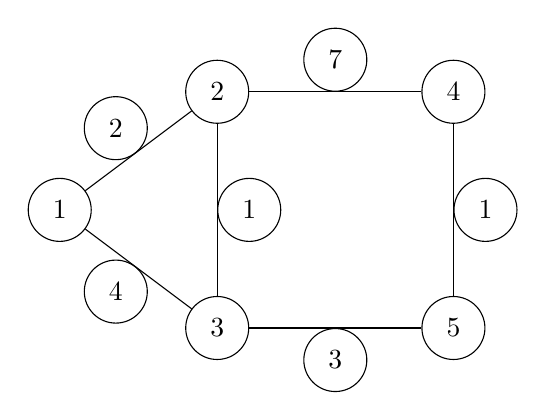
\begin{tikzpicture}[scale=1, every node/.style={circle, draw, minimum size=8mm}]
\node (1) at (0,0) {1};
\node (2) at (2,1.5) {2};
\node (3) at (2,-1.5) {3};
\node (4) at (5,1.5) {4};
\node (5) at (5,-1.5) {5};

\draw (1) -- (2) node[midway, above left] {2};
\draw (1) -- (3) node[midway, below left] {4};
\draw (2) -- (3) node[midway, right] {1};
\draw (2) -- (4) node[midway, above] {7};
\draw (3) -- (5) node[midway, below] {3};
\draw (4) -- (5) node[midway, right] {1};
\end{tikzpicture}

\chapter{Pemodelan Hubungan Dua Orang Pasangan (Pernikahan)}

\section{Pendahuluan}

Pernikahan adalah salah satu bentuk hubungan sosial yang paling fundamental dalam kehidupan manusia. 
Hubungan ini tidak hanya berakar pada aspek biologis dan emosional, tetapi juga dipengaruhi oleh faktor sosial, budaya, dan bahkan ekonomi. 
Meskipun demikian, di balik kompleksitas tersebut, terdapat pola-pola tertentu yang dapat diamati dalam interaksi antara suami dan istri. 
Matematika, khususnya pemodelan matematika, memberikan cara untuk merepresentasikan pola-pola tersebut secara kuantitatif sehingga kita dapat mempelajari bagaimana kasih sayang, perhatian, atau tingkat kepuasan dalam hubungan berubah seiring waktu.

Pada bab ini, kita akan membahas sebuah model matematis sederhana yang mencoba menangkap dinamika kasih sayang dalam hubungan pernikahan. 
Model ini didasarkan pada ide bahwa perasaan seorang individu terhadap pasangannya tidak berdiri sendiri, melainkan dipengaruhi oleh perilaku dan perasaan pasangannya. 
Jika suami menunjukkan kasih sayang, maka istri akan merespons dengan meningkatkan perasaan positifnya, demikian pula sebaliknya. 
Sebaliknya, jika tidak ada perhatian atau kasih sayang yang diberikan, maka perasaan tersebut cenderung memudar dengan berjalannya waktu. 

Dengan menggunakan sistem persamaan diferensial, kita dapat menyatakan perubahan tingkat kasih sayang tersebut dalam bentuk matematis yang dapat dianalisis secara sistematis. 
Meskipun model ini bersifat sederhana dan tentu saja jauh dari gambaran lengkap realitas kehidupan rumah tangga, ia dapat memberikan wawasan yang menarik tentang bagaimana interaksi timbal balik dalam suatu pasangan dapat mengarah pada hubungan yang harmonis, hubungan yang dingin, atau bahkan hubungan yang tidak stabil. 
Bab ini sekaligus menunjukkan bahwa pendekatan matematis dapat diterapkan tidak hanya pada fenomena alam atau ekonomi, tetapi juga pada aspek-aspek sosial dan psikologis manusia.

\section{Model Dasar: Dinamika Kasih Sayang}

Untuk dapat merepresentasikan hubungan pernikahan secara matematis, kita perlu terlebih dahulu menentukan variabel apa yang akan digunakan untuk menggambarkan keadaan pasangan tersebut. 
Dalam model sederhana ini, kita akan menggunakan dua variabel utama: 
\begin{itemize}
  \item $x(t)$ : tingkat kasih sayang atau perhatian suami terhadap istri pada waktu $t$,
  \item $y(t)$ : tingkat kasih sayang atau perhatian istri terhadap suami pada waktu $t$.
\end{itemize}

Kedua variabel ini dianggap sebagai besaran kontinu yang dapat meningkat atau menurun seiring berjalannya waktu. 
Tentu saja, dalam kenyataan, kasih sayang tidak dapat diukur secara langsung dalam angka, tetapi model ini menganggap bahwa terdapat suatu cara untuk merepresentasikannya secara kuantitatif. 
Dengan demikian, $x(t)$ dan $y(t)$ dapat dipandang sebagai indikator tingkat emosi yang dapat berubah secara dinamis.

Intuisi dasar dari model ini adalah bahwa perubahan perasaan seseorang terhadap pasangannya ditentukan oleh dua faktor utama. 
Pertama, ada pengaruh \emph{resiprokal} dari pasangannya. 
Sebagai contoh, jika istri menunjukkan perhatian lebih kepada suami, maka perasaan suami terhadap istri cenderung meningkat. 
Sebaliknya, jika suami tidak mendapatkan perhatian, maka perasaannya tidak akan bertambah karena tidak ada stimulus dari pihak lain. 
Kedua, ada kecenderungan alami bahwa setiap bentuk perhatian atau kasih sayang dapat memudar jika tidak dipupuk secara terus-menerus. 
Inilah yang disebut faktor \emph{peluruhan} dalam model.

Kedua mekanisme ini dapat diformulasikan dalam bentuk persamaan diferensial sederhana. 
Untuk suami, laju perubahan kasih sayang $x(t)$ dapat ditulis sebagai:
\begin{equation}
\frac{dx}{dt} = a y - b x,
\end{equation}
sedangkan untuk istri:
\begin{equation}
\frac{dy}{dt} = c x - d y.
\end{equation}

Di sini, parameter $a, b, c, d$ adalah bilangan positif yang memiliki interpretasi sebagai berikut:
\begin{itemize}
  \item $a$ : tingkat respons suami terhadap kasih sayang istrinya,
  \item $b$ : tingkat peluruhan perasaan suami ketika tidak mendapat perhatian,
  \item $c$ : tingkat respons istri terhadap kasih sayang suaminya,
  \item $d$ : tingkat peluruhan perasaan istri ketika tidak mendapat perhatian.
\end{itemize}

Model ini, walaupun sederhana, sudah cukup untuk menangkap gagasan inti: hubungan suami--istri adalah sebuah sistem timbal balik yang saling memengaruhi, di mana masing-masing individu akan menyesuaikan tingkat kasih sayangnya bergantung pada respons pasangannya sekaligus faktor internal dirinya sendiri. 
Dengan kerangka ini, kita dapat melanjutkan pada analisis titik kesetimbangan, yaitu keadaan di mana hubungan mencapai kondisi yang stabil.

\section{Titik Kesetimbangan}

Setelah merumuskan persamaan diferensial yang menggambarkan perubahan kasih sayang suami dan istri, langkah berikutnya adalah mencari \emph{titik kesetimbangan}. 
Titik kesetimbangan menggambarkan suatu kondisi di mana intensitas kasih sayang tidak lagi berubah seiring waktu. 
Dengan kata lain, jika pasangan sudah mencapai titik ini, maka interaksi kasih sayang mereka menjadi stabil, baik itu dalam bentuk hubungan yang harmonis, dingin, maupun kondisi lain yang bergantung pada parameter sistem.

Secara matematis, titik kesetimbangan dicapai ketika:
\[
\frac{dx}{dt} = 0, \qquad \frac{dy}{dt} = 0.
\]

Dengan mensubstitusikan persamaan model yang telah ditetapkan sebelumnya, diperoleh:
\[
a y - b x = 0, \qquad c x - d y = 0.
\]

Persamaan pertama dapat disusun kembali menjadi:
\[
a y = b x \quad \Rightarrow \quad y = \frac{b}{a}x.
\]

Demikian pula, persamaan kedua dapat ditulis ulang menjadi:
\[
c x = d y \quad \Rightarrow \quad y = \frac{c}{d}x.
\]

Dari dua hubungan ini, terlihat bahwa titik kesetimbangan yang mungkin terjadi sangat bergantung pada hubungan antara parameter $a$, $b$, $c$, dan $d$. 
Agar kedua kondisi tersebut konsisten, maka harus berlaku:
\[
\frac{b}{a} = \frac{c}{d} \quad \Rightarrow \quad ad = bc.
\]

Jika syarat $ad = bc$ terpenuhi, maka terdapat garis kesetimbangan berupa:
\[
y = \frac{b}{a}x.
\]
Hal ini menunjukkan bahwa ada banyak pasangan nilai $(x,y)$ yang dapat menjadi titik kesetimbangan, tergantung nilai awal yang dimiliki. 
Dengan kata lain, pasangan dapat mencapai berbagai kondisi stabil, asalkan proporsi kasih sayang mereka memenuhi hubungan di atas.

Sebaliknya, jika syarat $ad = bc$ tidak terpenuhi, maka satu-satunya titik kesetimbangan yang muncul adalah:
\[
(x^*, y^*) = (0,0).
\]

Secara interpretasi, kondisi $(0,0)$ menggambarkan sebuah hubungan di mana kedua belah pihak tidak lagi memiliki kasih sayang satu sama lain. 
Walaupun ini mungkin terdengar ekstrem, secara matematis titik ini tetap valid sebagai sebuah kesetimbangan. 
Artinya, tanpa adanya respons yang seimbang antara suami dan istri, hubungan mereka akan menuju kondisi \emph{dingin} di mana kasih sayang hilang sepenuhnya.

Dengan demikian, analisis titik kesetimbangan ini menunjukkan bahwa keberlangsungan sebuah hubungan dalam model ini sangat bergantung pada keseimbangan respons antara kedua belah pihak. 
Apabila keduanya seimbang, maka berbagai kondisi stabil dapat tercapai. 
Namun, jika keseimbangan tersebut tidak ada, maka hubungan cenderung berakhir pada kondisi yang tidak menyenangkan.

\section{Analisis Stabilitas}

Mengetahui titik kesetimbangan saja belum cukup untuk memahami dinamika hubungan suami--istri dalam model ini. 
Kita juga perlu mempelajari apakah titik kesetimbangan tersebut bersifat \emph{stabil} atau \emph{tidak stabil}. 
Stabilitas menentukan apakah kondisi kasih sayang yang dicapai akan bertahan lama, ataukah justru mudah goyah akibat sedikit gangguan. 
Dalam konteks pernikahan, stabilitas dapat ditafsirkan sebagai kekuatan hubungan menghadapi perubahan kecil dalam interaksi sehari-hari.

Untuk menganalisis stabilitas, kita menggunakan pendekatan sistem dinamik linier dengan matriks Jacobian. 
Jacobian diperoleh dari turunan parsial sistem terhadap variabel $x$ dan $y$:
\[
J = 
\begin{pmatrix}
\frac{\partial}{\partial x}\left( \frac{dx}{dt} \right) & \frac{\partial}{\partial y}\left( \frac{dx}{dt} \right) \\[6pt]
\frac{\partial}{\partial x}\left( \frac{dy}{dt} \right) & \frac{\partial}{\partial y}\left( \frac{dy}{dt} \right)
\end{pmatrix}.
\]

Dengan mensubstitusi sistem yang ada, diperoleh:
\[
J = 
\begin{pmatrix}
-b & a \\
c & -d
\end{pmatrix}.
\]

Karakteristik stabilitas ditentukan oleh nilai eigen dari matriks Jacobian tersebut. 
Nilai eigen dihitung dari persamaan karakteristik:
\[
\det(J - \lambda I) = 0,
\]
atau
\[
\begin{vmatrix}
-b - \lambda & a \\
c & -d - \lambda
\end{vmatrix} = 0.
\]

Hasil perhitungan memberikan:
\[
\lambda^2 + (b+d)\lambda + (bd - ac) = 0.
\]

Sehingga nilai eigen adalah:
\[
\lambda = \frac{-(b+d) \pm \sqrt{(b-d)^2 + 4ac}}{2}.
\]

Analisis terhadap tanda dari nilai eigen ini memberikan informasi sebagai berikut:
\begin{itemize}
  \item Jika kedua nilai eigen memiliki bagian real negatif, maka sistem stabil. 
  Artinya, meskipun ada gangguan kecil, kasih sayang pasangan akan kembali menuju titik kesetimbangan. 
  Dalam konteks hubungan, ini menggambarkan \textbf{pernikahan yang kuat dan harmonis}.
  \item Jika salah satu nilai eigen memiliki bagian real positif, maka sistem tidak stabil. 
  Gangguan kecil akan menyebabkan dinamika kasih sayang menjauh dari titik kesetimbangan. 
  Secara sosial, ini dapat diartikan sebagai \textbf{hubungan yang rapuh}, di mana konflik kecil dapat membesar hingga merusak kestabilan hubungan.
  \item Jika nilai eigen berupa bilangan kompleks dengan bagian real negatif, maka sistem akan mengalami osilasi yang berangsur-angsur mereda menuju titik kesetimbangan. 
  Ini dapat ditafsirkan sebagai \textbf{hubungan yang mengalami pasang surut}, tetapi pada akhirnya kembali stabil.
  \item Jika nilai eigen berupa bilangan kompleks dengan bagian real positif, sistem akan berosilasi semakin menjauh dari titik kesetimbangan. 
  Dalam kehidupan nyata, ini dapat menggambarkan \textbf{hubungan yang penuh gejolak}, di mana konflik dan rekonsiliasi berulang namun makin lama makin memperburuk keadaan.
\end{itemize}

Dengan demikian, stabilitas dalam model ini sepenuhnya ditentukan oleh parameter $a$, $b$, $c$, dan $d$. 
Respons positif yang kuat dari masing-masing pasangan ($a$ dan $c$ besar) cenderung mendukung kestabilan, selama diimbangi dengan tingkat peluruhan ($b$ dan $d$) yang tidak terlalu besar. 
Namun, jika keseimbangan parameter tidak tercapai, hubungan dapat bergerak ke arah instabilitas yang pada akhirnya merusak ikatan pernikahan.

\section{Interpretasi dalam Konteks Pernikahan}

Setelah kita mengetahui titik kesetimbangan dan sifat stabilitasnya, langkah berikutnya adalah memberikan interpretasi sosial terhadap hasil matematis tersebut. 
Model sederhana ini pada dasarnya berusaha menangkap dinamika emosional antara suami dan istri dalam bentuk angka. 
Walaupun jelas bahwa kehidupan rumah tangga jauh lebih kompleks, analisis matematis dapat memberikan gambaran konseptual mengenai kemungkinan pola hubungan yang terjadi.

\subsection*{Hubungan Harmonis}
Kondisi harmonis terjadi ketika kedua pasangan memiliki parameter respons yang cukup besar ($a$ dan $c$), sementara tingkat peluruhan ($b$ dan $d$) relatif kecil. 
Artinya, baik suami maupun istri cenderung cepat merespons kasih sayang pasangannya, dan pada saat yang sama tidak mudah melupakan atau kehilangan rasa sayang tersebut. 
Dalam situasi ini, titik kesetimbangan yang stabil menggambarkan hubungan di mana kasih sayang bertahan dalam jangka panjang. 
Meskipun mungkin terdapat pasang surut, hubungan akan selalu kembali menuju keadaan seimbang yang penuh kehangatan.

\subsection*{Hubungan Dingin}
Sebaliknya, jika nilai $b$ dan $d$ jauh lebih besar daripada $a$ dan $c$, maka kasih sayang cenderung cepat memudar tanpa cukup respons dari pasangan. 
Dalam kasus ini, titik kesetimbangan yang tercapai biasanya adalah $(0,0)$, yang secara metaforis menggambarkan keadaan \emph{hubungan dingin}. 
Pasangan mungkin tetap bersama secara formal, tetapi interaksi emosional mereka lemah, sehingga cinta dan perhatian hampir tidak ada lagi. 
Hal ini dapat diartikan sebagai pernikahan yang kehilangan makna emosionalnya.

\subsection*{Hubungan Tidak Seimbang}
Ada pula kemungkinan bahwa salah satu pasangan memiliki tingkat respons yang jauh lebih besar dibandingkan pasangannya. 
Misalnya, jika $a \gg c$, maka kasih sayang suami akan sangat bergantung pada perhatian istrinya, sementara istri kurang merespons kasih sayang suaminya. 
Situasi ini menciptakan hubungan yang \emph{tidak seimbang}, di mana salah satu pihak merasa selalu memberi lebih banyak daripada yang diterima. 
Dalam jangka panjang, hal ini dapat menimbulkan ketidakpuasan atau bahkan konflik.

\subsection*{Hubungan Gejolak}
Dalam beberapa kasus, nilai eigen yang diperoleh berupa bilangan kompleks dengan bagian real positif. 
Artinya, hubungan mengalami osilasi yang semakin lama semakin membesar. 
Interpretasinya adalah pasangan mengalami pola \emph{cinta-benci} yang berulang: pada suatu waktu mereka sangat dekat, kemudian berkonflik hebat, lalu kembali mesra, dan seterusnya. 
Namun, seiring berjalannya waktu, konflik dan rekonsiliasi ini tidak menuntun pada stabilitas, melainkan pada gejolak yang makin intens. 
Situasi semacam ini dalam dunia nyata kerap kali berakhir dengan perpisahan.

\subsection*{Kesimpulan Sementara}
Dari analisis ini, kita dapat menyimpulkan bahwa kestabilan hubungan pernikahan dalam model bergantung pada keseimbangan antara \emph{respons positif} dan \emph{peluruhan kasih sayang}. 
Hubungan yang sehat membutuhkan kedua pihak untuk sama-sama responsif terhadap kasih sayang yang diberikan sekaligus memiliki daya tahan emosional. 
Jika salah satu aspek ini lemah atau tidak seimbang, maka hubungan cenderung rapuh dan tidak stabil. 
Meskipun model ini sederhana, ia berhasil menyoroti prinsip penting: keberlangsungan sebuah hubungan tidak hanya ditentukan oleh seberapa besar kasih sayang awal, tetapi juga oleh bagaimana kasih sayang tersebut dipelihara dan direspons secara timbal balik.

\section{Ekstensi Model}

Model dasar yang telah dibahas sebelumnya sangat sederhana: hanya dua variabel $x(t)$ dan $y(t)$ yang saling memengaruhi dengan aturan linier. 
Walaupun cukup untuk memberikan intuisi awal, tentu kehidupan pernikahan jauh lebih rumit dibandingkan model linier dua variabel. 
Oleh karena itu, penting untuk memikirkan bagaimana model ini dapat diperluas (\emph{extended}) agar lebih realistis dan mampu menangkap aspek-aspek lain dalam dinamika hubungan.

\subsection*{Pengaruh Faktor Eksternal}
Dalam kenyataan, hubungan pernikahan tidak berlangsung dalam ruang hampa, melainkan dipengaruhi oleh banyak faktor eksternal. 
Sebagai contoh, keberadaan anak, campur tangan keluarga besar, tekanan pekerjaan, maupun kondisi ekonomi dapat memengaruhi intensitas kasih sayang pasangan. 
Untuk memodelkan hal ini, kita dapat menambahkan variabel baru $z(t)$ yang mewakili pengaruh faktor eksternal tersebut. 
Dengan demikian, sistem persamaan dapat ditulis menjadi:
\[
\frac{dx}{dt} = a y - b x + e z, \qquad
\frac{dy}{dt} = c x - d y + f z,
\]
di mana $e$ dan $f$ menyatakan seberapa besar pengaruh faktor eksternal terhadap kasih sayang masing-masing pihak. 
Misalnya, anak yang baru lahir dapat meningkatkan kehangatan keluarga (nilai $e$ dan $f$ positif), sementara tekanan ekonomi justru dapat mengurangi kasih sayang (nilai $e$ dan $f$ negatif).

\subsection*{Efek Komunikasi Diskrit}
Interaksi dalam pernikahan sering kali terjadi secara diskrit, misalnya melalui percakapan harian, pertemuan mingguan, atau momen-momen penting tertentu. 
Untuk merepresentasikan hal ini, model diferensial dapat diubah menjadi model \emph{diskrit} dengan persamaan rekurensi:
\[
x_{n+1} = (1-b)x_n + a y_n, \qquad
y_{n+1} = (1-d)y_n + c x_n.
\]
Di sini, $x_n$ dan $y_n$ menyatakan tingkat kasih sayang pada waktu diskrit ke-$n$. 
Model diskrit semacam ini sering kali memperlihatkan perilaku yang berbeda dari model kontinu, misalnya adanya osilasi tajam atau bahkan perilaku kacau (\emph{chaotic}) pada parameter tertentu. 
Hal ini dapat ditafsirkan sebagai pasangan yang mengalami naik-turun perasaan secara drastis dari waktu ke waktu.

\subsection*{Model Nonlinier}
Hubungan antar manusia jarang sekali bersifat linier. 
Sebagai contoh, jika salah satu pihak sudah menunjukkan kasih sayang yang sangat besar, respons pasangannya mungkin tidak lagi bertambah secara proporsional, melainkan cenderung jenuh. 
Fenomena ini dapat dimodelkan dengan menambahkan fungsi nonlinier, misalnya fungsi logistik atau fungsi saturasi:
\[
\frac{dx}{dt} = \frac{a y}{1 + \alpha y^2} - b x, \qquad
\frac{dy}{dt} = \frac{c x}{1 + \beta x^2} - d y.
\]
Dengan modifikasi ini, model dapat menangkap kenyataan bahwa ada batasan psikologis dalam merespons kasih sayang pasangan.

\subsection*{Pendekatan Stokastik dan Berbasis Agen}
Dalam kenyataan, manusia tidak selalu konsisten dalam bertindak. 
Kadang-kadang kasih sayang meningkat atau menurun akibat faktor acak seperti suasana hati, kesehatan, atau kejadian mendadak. 
Untuk merepresentasikan hal ini, model stokastik dapat digunakan dengan menambahkan \emph{noise} acak ke dalam persamaan diferensial:
\[
\frac{dx}{dt} = a y - b x + \sigma_1 \xi_1(t), \qquad
\frac{dy}{dt} = c x - d y + \sigma_2 \xi_2(t),
\]
di mana $\xi_1(t)$ dan $\xi_2(t)$ adalah proses stokastik (misalnya \emph{white noise}), dan $\sigma_1$, $\sigma_2$ adalah parameter intensitas gangguan acak. 

Selain itu, pendekatan \emph{agent-based modeling} (ABM) juga dapat digunakan untuk memodelkan banyak pasangan sekaligus. 
Dalam pendekatan ini, setiap pasangan (agen) memiliki parameter $a$, $b$, $c$, dan $d$ yang berbeda-beda sesuai karakter mereka. 
Dengan simulasi komputer, dapat dipelajari bagaimana interaksi antar banyak pasangan menghasilkan pola sosial yang lebih besar, misalnya tingkat perceraian atau kebahagiaan dalam sebuah komunitas.

\subsection*{Ringkasan}
Ekstensi-ekstensi ini menunjukkan bahwa model dasar hanyalah titik awal. 
Dengan menambahkan faktor eksternal, efek diskrit, nonlinieritas, serta unsur stokastik, kita dapat membuat model yang lebih kaya dan mendekati realitas. 
Namun, semakin kompleks model, semakin sulit pula melakukan analisis matematis secara analitik, sehingga simulasi numerik menjadi alat yang sangat penting.

\section{Simulasi Numerik}

Analisis matematis memberikan gambaran umum mengenai titik kesetimbangan dan stabilitas sistem. 
Namun, untuk memperoleh pemahaman yang lebih konkret mengenai dinamika kasih sayang, kita dapat melakukan \emph{simulasi numerik}. 
Simulasi memungkinkan kita untuk melihat bagaimana nilai $x(t)$ dan $y(t)$ berubah seiring waktu, berdasarkan parameter yang dipilih dan kondisi awal tertentu. 
Dengan cara ini, model yang abstrak dapat divisualisasikan sehingga lebih mudah diinterpretasikan dalam konteks kehidupan nyata.

\subsection*{Kasus Dasar: Respons Seimbang}
Pertimbangkan parameter berikut:
\[
a = 2, \quad b = 1, \quad c = 2, \quad d = 1.
\]
Dengan nilai ini, baik suami maupun istri memiliki tingkat respons yang sama terhadap pasangannya, dan tingkat peluruhan yang sama pula. 
Jika kita ambil kondisi awal $x(0) = 1$ dan $y(0) = 0.5$, simulasi numerik menunjukkan bahwa nilai $x(t)$ dan $y(t)$ akan mengalami osilasi yang berangsur-angsur mereda, sebelum akhirnya mendekati suatu titik kesetimbangan. 
Secara sosial, hal ini dapat ditafsirkan sebagai hubungan yang mengalami pasang surut kecil, tetapi pada akhirnya mencapai kestabilan yang harmonis.

\subsection*{Kasus Tidak Seimbang: Suami Lebih Responsif}
Sekarang kita pilih parameter:
\[
a = 3, \quad b = 1, \quad c = 1, \quad d = 1.
\]
Dalam hal ini, suami ($x$) jauh lebih responsif terhadap kasih sayang istrinya dibandingkan sebaliknya. 
Hasil simulasi memperlihatkan bahwa $x(t)$ meningkat dengan cepat, sedangkan $y(t)$ tidak bertambah secara signifikan. 
Dinamika ini menggambarkan hubungan yang tidak seimbang, di mana salah satu pihak lebih “mencintai” dibandingkan yang lain. 
Jika situasi ini berlangsung lama, hubungan dapat menjadi tidak stabil karena ketimpangan dalam interaksi emosional.

\subsection*{Kasus Gejolak: Parameter Mendorong Osilasi Membesar}
Terakhir, ambil parameter:
\[
a = 2, \quad b = 0.2, \quad c = 2, \quad d = 0.2.
\]
Nilai peluruhan yang sangat kecil ($b$ dan $d$) digabungkan dengan respons besar ($a$ dan $c$) menghasilkan dinamika yang berosilasi dengan amplitudo semakin membesar. 
Simulasi memperlihatkan naik-turun drastis antara $x(t)$ dan $y(t)$. 
Interpretasinya adalah pasangan mengalami hubungan penuh gejolak: mereka bisa sangat mesra pada suatu waktu, tetapi kemudian terjebak dalam konflik hebat, dan siklus ini terus berulang dengan intensitas yang makin besar.

\subsection*{Visualisasi dengan Komputer}
Simulasi numerik dapat dengan mudah dilakukan menggunakan perangkat lunak seperti Python, MATLAB, atau Octave. 
Sebagai contoh, menggunakan Python dengan pustaka \texttt{matplotlib}, kita dapat menggambarkan kurva $x(t)$ dan $y(t)$ sebagai fungsi waktu. 
Grafik yang dihasilkan memberikan intuisi visual: apakah kasih sayang cenderung stabil, memudar, atau bergejolak. 

Selain itu, visualisasi fase (\emph{phase portrait}) juga sangat informatif. 
Dengan menggambarkan lintasan $(x(t), y(t))$ dalam bidang dua dimensi, kita dapat melihat pola interaksi antara suami dan istri. 
Lintasan yang menuju satu titik menunjukkan stabilitas, sedangkan lintasan yang menjauh atau berosilasi tanpa henti menunjukkan instabilitas atau dinamika kompleks.

\subsection*{Ringkasan}
Simulasi numerik menegaskan bahwa perilaku sistem sangat bergantung pada nilai parameter. 
Hubungan yang seimbang menghasilkan kestabilan, hubungan yang timpang menghasilkan ketidakpuasan, dan hubungan dengan respons terlalu besar dapat berakhir dalam gejolak. 
Dengan demikian, simulasi memberikan bukti visual sekaligus memperkaya interpretasi matematis yang telah kita peroleh sebelumnya.

\section{Penutup}

Bab ini memperlihatkan bahwa meskipun hubungan pernikahan merupakan fenomena yang sangat kompleks, matematika dapat memberikan kerangka sederhana untuk memahami dinamika di dalamnya. 
Dengan memperkenalkan variabel $x(t)$ dan $y(t)$ sebagai tingkat kasih sayang suami dan istri, serta menggunakan sistem persamaan diferensial linier, kita mampu menggambarkan bagaimana kasih sayang tersebut berubah seiring waktu. 
Hasil analisis menunjukkan bahwa hubungan dapat mencapai titik kesetimbangan yang stabil, menjadi dingin tanpa kasih sayang, atau bahkan bergejolak, bergantung pada nilai parameter yang mewakili respons dan peluruhan masing-masing pihak.

Interpretasi sosial dari model ini menekankan pentingnya keseimbangan antara \emph{respons positif} dan \emph{daya tahan emosional}. 
Hubungan yang sehat membutuhkan kedua belah pihak untuk sama-sama responsif terhadap kasih sayang pasangannya, sekaligus memiliki kemampuan untuk menjaga perasaan agar tidak mudah memudar. 
Jika salah satu aspek ini tidak terpenuhi, maka hubungan menjadi rapuh dan cenderung tidak stabil. 
Walaupun model ini hanya menyajikan gambaran yang sangat sederhana, pesan moral yang terkandung di dalamnya tetap relevan: cinta perlu dipupuk dan dijaga secara timbal balik agar hubungan tetap harmonis.

Selain itu, bab ini juga menunjukkan bahwa model dapat diperluas untuk mencakup pengaruh faktor eksternal, interaksi diskrit, nonlinieritas, maupun unsur stokastik. 
Dengan pendekatan tersebut, kita dapat menangkap realitas yang lebih kaya, meskipun analisis matematis menjadi lebih sulit dan sering kali memerlukan simulasi komputer. 
Hasil simulasi numerik yang ditampilkan memperlihatkan secara visual berbagai kemungkinan perilaku hubungan, mulai dari kestabilan hingga gejolak emosional.

Akhirnya, bab ini memberikan bukti nyata bahwa pemodelan matematika tidak terbatas pada bidang-bidang tradisional seperti biologi, fisika, atau ekonomi, melainkan juga dapat diterapkan pada fenomena sosial dan psikologis. 
Dengan demikian, pemodelan hubungan pasangan suami--istri bukan hanya sekadar latihan akademis, tetapi juga sebuah ilustrasi menarik tentang bagaimana matematika dapat membantu kita merenungkan aspek-aspek penting dari kehidupan manusia.

\chapter{Pemodelan Gelombang Linier}

\section{Pendahuluan}

Gelombang merupakan salah satu fenomena alam yang paling sering kita jumpai dalam kehidupan sehari-hari. 
Mulai dari gelombang air di lautan, gelombang bunyi yang kita dengar, hingga gelombang cahaya yang memungkinkan kita melihat, semuanya dapat dipandang sebagai contoh nyata dari propagasi energi melalui suatu medium. 
Untuk memahami fenomena tersebut, matematika memberikan kerangka yang kuat melalui teori gelombang.

Dalam bab ini, kita akan mempelajari model matematis untuk \emph{gelombang linier}. 
Disebut linier karena persamaan yang digunakan memiliki sifat superposisi: jika dua gelombang merupakan solusi, maka penjumlahan keduanya juga merupakan solusi. 
Sifat ini sangat penting karena memungkinkan kita menganalisis gelombang yang kompleks sebagai kombinasi dari gelombang-gelombang sederhana.

Model gelombang linier menjadi landasan penting sebelum kita melangkah ke model yang lebih kompleks seperti gelombang nonlinier atau gelombang soliter. 
Meskipun terlihat sederhana, teori gelombang linier telah berhasil menjelaskan berbagai fenomena dengan akurasi tinggi, mulai dari propagasi suara hingga desain teknologi komunikasi. 
Oleh karena itu, pemahaman yang kuat tentang model ini merupakan fondasi untuk mempelajari gelombang dalam bentuk yang lebih maju.

\section{Persamaan Gelombang Linier Dasar}

Untuk memodelkan gelombang linier, kita memulai dari hukum fisika dasar, yaitu hukum Newton tentang gerak dan hukum Hooke tentang elastisitas. 
Kombinasi keduanya menghasilkan suatu persamaan diferensial parsial (PDP) yang dikenal sebagai \emph{persamaan gelombang}.

\subsection{Turunan dari Kasus Tali Tegang}

Misalkan kita memiliki sebuah tali panjang yang tegang dengan gaya tegangan $T$, dan massa jenis linear $\mu$ (massa per satuan panjang). 
Jika $u(x,t)$ menyatakan simpangan tali dari posisi kesetimbangannya pada titik $x$ dan waktu $t$, maka gaya yang bekerja pada elemen tali sepanjang $\Delta x$ dapat dituliskan sebagai selisih gaya tegangan pada ujung-ujungnya. 
Dengan menggunakan pendekatan kalkulus, diperoleh:
\[
\mu \, \Delta x \, \frac{\partial^2 u}{\partial t^2} 
= T \left( \frac{\partial u}{\partial x}\bigg|_{x+\Delta x} - \frac{\partial u}{\partial x}\bigg|_{x} \right).
\]

Dengan mengambil limit $\Delta x \to 0$, kita mendapatkan persamaan diferensial parsial:
\[
\mu \frac{\partial^2 u}{\partial t^2} = T \frac{\partial^2 u}{\partial x^2}.
\]

Jika kita definisikan kecepatan rambat gelombang sebagai
\[
c = \sqrt{\frac{T}{\mu}},
\]
maka persamaan di atas dapat ditulis lebih sederhana menjadi:
\begin{equation}
\frac{\partial^2 u}{\partial t^2} = c^2 \frac{\partial^2 u}{\partial x^2}.
\end{equation}

Persamaan ini dikenal sebagai \textbf{persamaan gelombang satu dimensi}. 
Solusi dari persamaan ini menggambarkan bagaimana gelombang merambat sepanjang tali.

\subsection*{Solusi Umum Persamaan Gelombang}
D’Alembert menunjukkan bahwa solusi umum dari persamaan gelombang satu dimensi adalah:
\[
u(x,t) = f(x-ct) + g(x+ct),
\]
dengan $f$ dan $g$ fungsi sembarang yang cukup halus. 
Secara fisik, $f(x-ct)$ mewakili gelombang yang merambat ke arah kanan dengan kecepatan $c$, sedangkan $g(x+ct)$ mewakili gelombang yang merambat ke arah kiri dengan kecepatan $c$. 

Artinya, setiap bentuk gelombang awal dapat dianggap sebagai kombinasi dari dua gelombang yang bergerak ke arah berlawanan tanpa mengalami perubahan bentuk. 
Hal inilah yang disebut sifat linier: gelombang dapat ditumpuk tanpa saling memengaruhi.

\subsection*{Ekstensi ke Dua dan Tiga Dimensi}
Persamaan gelombang dapat diperluas ke ruang dua dimensi dan tiga dimensi. 
Dalam notasi umum, persamaan gelombang dapat ditulis sebagai:
\[
\frac{\partial^2 u}{\partial t^2} = c^2 \nabla^2 u,
\]
dengan $\nabla^2$ adalah operator Laplace. 
Dalam koordinat kartesian tiga dimensi, bentuk lengkapnya adalah:
\[
\frac{\partial^2 u}{\partial t^2} = c^2 \left( 
\frac{\partial^2 u}{\partial x^2} + 
\frac{\partial^2 u}{\partial y^2} + 
\frac{\partial^2 u}{\partial z^2}
\right).
\]

Persamaan ini merupakan dasar bagi pemodelan berbagai fenomena gelombang, mulai dari bunyi dalam udara, gelombang air, hingga gelombang elektromagnetik dalam ruang hampa.

\section{Kondisi Batas dan Awal}

Persamaan gelombang yang telah kita peroleh tidak akan lengkap tanpa menentukan kondisi tambahan yang disebut \emph{kondisi batas} (boundary conditions) dan \emph{kondisi awal} (initial conditions). 
Kondisi-kondisi ini sangat penting karena merepresentasikan keadaan fisik sistem yang sedang dipelajari, serta memastikan bahwa solusi yang diperoleh bersifat unik dan sesuai dengan kenyataan.

\subsection*{Kondisi Awal}
Kondisi awal menggambarkan keadaan sistem pada waktu $t=0$. 
Untuk sistem tali, biasanya terdapat dua jenis informasi awal:
\begin{enumerate}
  \item Bentuk awal tali, yang dituliskan sebagai:
  \[
  u(x,0) = f(x),
  \]
  di mana $f(x)$ adalah fungsi yang mendeskripsikan posisi tali pada saat awal.
  \item Kecepatan awal setiap titik pada tali, yang dituliskan sebagai:
  \[
  \frac{\partial u}{\partial t}(x,0) = g(x),
  \]
  di mana $g(x)$ adalah fungsi yang menunjukkan bagaimana tali sedang digerakkan pada saat awal.
\end{enumerate}

Dengan dua informasi ini, kita dapat menentukan evolusi gelombang pada waktu selanjutnya secara unik.

\subsection*{Kondisi Batas}
Kondisi batas menjelaskan bagaimana ujung-ujung medium diperlakukan. 
Untuk tali, ada beberapa kemungkinan kondisi batas yang umum digunakan:
\begin{itemize}
  \item \textbf{Ujung terikat:} jika ujung tali dipaku atau dijepit, maka simpangan di ujung selalu nol:
  \[
  u(0,t) = 0, \qquad u(L,t) = 0.
  \]
  Kondisi ini sesuai dengan contoh tali gitar yang terikat di kedua ujungnya.
  \item \textbf{Ujung bebas:} jika ujung tali dibiarkan bebas, maka gradien simpangan di ujung bernilai nol:
  \[
  \frac{\partial u}{\partial x}(0,t) = 0, \qquad \frac{\partial u}{\partial x}(L,t) = 0.
  \]
  Kondisi ini lebih jarang dipakai dalam instrumen musik, tetapi relevan dalam eksperimen fisika.
  \item \textbf{Kombinasi:} satu ujung terikat dan satu ujung bebas, misalnya pada beberapa jenis antena atau sistem mekanik.
\end{itemize}

\subsection*{Contoh Fisik: Tali Gitar}
Kasus klasik adalah getaran tali gitar sepanjang $L$ dengan kedua ujung terikat. 
Kondisi batasnya adalah:
\[
u(0,t) = 0, \qquad u(L,t) = 0.
\]
Jika pada awalnya tali digetarkan dengan bentuk tertentu $f(x)$ dan kecepatan awal nol ($g(x)=0$), maka evolusi getarannya dapat diprediksi dengan persamaan gelombang.

\subsection*{Prinsip Superposisi}
Karena persamaan gelombang linier, solusi umum yang memenuhi kondisi awal dan batas dapat diperoleh sebagai superposisi dari solusi dasar. 
Dengan kata lain, bentuk gelombang yang kompleks dapat dipandang sebagai kombinasi dari gelombang sederhana. 
Prinsip inilah yang membuat teori gelombang linier sangat kuat: fenomena nyata yang rumit dapat diuraikan menjadi gelombang-gelombang dasar yang lebih mudah dipahami.

\section{Solusi dengan Pemisahan Variabel}

Salah satu metode yang paling umum digunakan untuk menyelesaikan persamaan gelombang linier adalah \emph{metode pemisahan variabel} (separation of variables). 
Metode ini bekerja dengan asumsi bahwa solusi $u(x,t)$ dapat ditulis sebagai hasil kali dari dua fungsi yang masing-masing hanya bergantung pada satu variabel:
\[
u(x,t) = X(x) T(t),
\]
dengan $X(x)$ hanya bergantung pada posisi dan $T(t)$ hanya bergantung pada waktu.

\subsection*{Substitusi ke dalam Persamaan Gelombang}
Kita mulai dengan persamaan gelombang satu dimensi:
\[
\frac{\partial^2 u}{\partial t^2} = c^2 \frac{\partial^2 u}{\partial x^2}.
\]
Dengan substitusi $u(x,t) = X(x) T(t)$, diperoleh:
\[
X(x) \frac{d^2 T}{dt^2} = c^2 T(t) \frac{d^2 X}{dx^2}.
\]

Membagi kedua ruas dengan $X(x)T(t)$ (diasumsikan $X,T \neq 0$), kita dapatkan:
\[
\frac{1}{T(t)} \frac{d^2 T}{dt^2} = c^2 \frac{1}{X(x)} \frac{d^2 X}{dx^2}.
\]

Karena ruas kiri hanya bergantung pada $t$ dan ruas kanan hanya bergantung pada $x$, maka keduanya harus sama dengan suatu konstanta. 
Kita pilih konstanta $-\lambda$ (negatif untuk memudahkan analisis gelombang):
\[
\frac{1}{T(t)} \frac{d^2 T}{dt^2} = -\lambda, 
\qquad
c^2 \frac{1}{X(x)} \frac{d^2 X}{dx^2} = -\lambda.
\]

\subsection*{Persamaan untuk $X(x)$}
Dari hubungan di atas, persamaan untuk $X(x)$ adalah:
\[
\frac{d^2 X}{dx^2} + \frac{\lambda}{c^2} X = 0.
\]
Kita definisikan $k^2 = \frac{\lambda}{c^2}$, sehingga persamaan menjadi:
\[
\frac{d^2 X}{dx^2} + k^2 X = 0.
\]
Solusi umum dari persamaan ini adalah:
\[
X(x) = A \sin(kx) + B \cos(kx),
\]
dengan $A$ dan $B$ konstanta.

\subsection*{Persamaan untuk $T(t)$}
Sementara itu, persamaan untuk $T(t)$ adalah:
\[
\frac{d^2 T}{dt^2} + \lambda T = 0.
\]
Dengan $\lambda = k^2 c^2$, solusinya adalah:
\[
T(t) = C \cos(kct) + D \sin(kct),
\]
dengan $C$ dan $D$ konstanta.

\subsection*{Solusi Umum}
Dengan menggabungkan hasil $X(x)$ dan $T(t)$, diperoleh solusi umum:
\[
u(x,t) = \big( A \sin(kx) + B \cos(kx) \big) \big( C \cos(kct) + D \sin(kct) \big).
\]

\subsection*{Penerapan pada Tali dengan Ujung Terikat}
Untuk kasus tali gitar sepanjang $L$ dengan ujung terikat, kita memiliki kondisi batas:
\[
u(0,t) = 0, \qquad u(L,t) = 0.
\]

Kondisi $u(0,t)=0$ memberikan syarat $B=0$. 
Sehingga fungsi $X(x)$ menyederhana menjadi:
\[
X(x) = A \sin(kx).
\]

Kondisi $u(L,t)=0$ menghasilkan:
\[
\sin(kL) = 0 \quad \Rightarrow \quad kL = n\pi, \qquad n = 1,2,3,\dots
\]

Dengan demikian, nilai $k$ yang diperbolehkan adalah:
\[
k_n = \frac{n\pi}{L}.
\]

Sehingga solusi untuk mode ke-$n$ adalah:
\[
u_n(x,t) = \sin\left(\frac{n\pi x}{L}\right) \Big( C_n \cos\left(\frac{n\pi c}{L} t\right) + D_n \sin\left(\frac{n\pi c}{L} t\right) \Big).
\]

\subsection*{Makna Fisik}
Hasil ini menunjukkan bahwa tali yang terikat di kedua ujungnya hanya dapat bergetar dalam \textbf{mode-mode diskrit} (disebut \emph{frekuensi natural} atau \emph{frekuensi eigen}). 
Mode pertama ($n=1$) disebut \emph{mode fundamental}, sedangkan $n=2,3,\dots$ disebut \emph{harmonik}. 
Inilah dasar ilmiah dari nada musik: setiap instrumen menghasilkan bunyi khas karena perbedaan frekuensi natural dari sistem fisiknya.

\section{Prinsip Superposisi dan Analisis Fourier}

Salah satu kekuatan utama dari persamaan gelombang linier adalah adanya \emph{prinsip superposisi}. 
Prinsip ini menyatakan bahwa jika $u_1(x,t)$ dan $u_2(x,t)$ merupakan solusi dari persamaan gelombang, maka kombinasi linear
\[
u(x,t) = \alpha u_1(x,t) + \beta u_2(x,t),
\]
dengan $\alpha$ dan $\beta$ konstanta sembarang, juga merupakan solusi. 
Prinsip ini membuat teori gelombang linier sangat fleksibel karena memungkinkan kita membangun solusi kompleks dari solusi-solusi sederhana.

\subsection*{Superposisi Mode Eigen}
Dari hasil sebelumnya, kita telah menemukan bahwa solusi persamaan gelombang dengan kondisi batas tali terikat di kedua ujungnya hanya mungkin dalam bentuk mode diskrit:
\[
u_n(x,t) = \sin\left(\frac{n\pi x}{L}\right) \Big( C_n \cos\left(\frac{n\pi c}{L} t\right) + D_n \sin\left(\frac{n\pi c}{L} t\right) \Big).
\]

Dengan prinsip superposisi, solusi umum dapat dituliskan sebagai kombinasi semua mode yang mungkin:
\[
u(x,t) = \sum_{n=1}^{\infty} \sin\left(\frac{n\pi x}{L}\right) 
\Big( C_n \cos\left(\frac{n\pi c}{L} t\right) + D_n \sin\left(\frac{n\pi c}{L} t\right) \Big).
\]

Persamaan ini menyatakan bahwa getaran tali sebenarnya adalah gabungan dari berbagai mode harmonik. 
Mode fundamental memberikan kontribusi dominan, sementara mode-mode lebih tinggi menambahkan variasi bentuk getaran.

\subsection*{Analisis Fourier}
Untuk menentukan koefisien $C_n$ dan $D_n$, kita perlu memperhatikan kondisi awal $u(x,0) = f(x)$ dan $\frac{\partial u}{\partial t}(x,0) = g(x)$. 
Dengan mensubstitusikan $t=0$, kita peroleh:
\[
f(x) = \sum_{n=1}^{\infty} C_n \sin\left(\frac{n\pi x}{L}\right),
\]
dan dari turunan waktu:
\[
g(x) = \sum_{n=1}^{\infty} \frac{n\pi c}{L} D_n \sin\left(\frac{n\pi x}{L}\right).
\]

Kedua ekspresi ini adalah contoh dari \textbf{deret Fourier sinus}. 
Artinya, bentuk awal tali $f(x)$ dapat direpresentasikan sebagai kombinasi dari fungsi sinus dengan frekuensi diskrit tertentu. 
Koefisien $C_n$ dan $D_n$ diperoleh dengan memproyeksikan $f(x)$ dan $g(x)$ ke basis sinus:
\[
C_n = \frac{2}{L} \int_0^L f(x) \sin\left(\frac{n\pi x}{L}\right) dx,
\]
\[
D_n = \frac{2}{n\pi c} \int_0^L g(x) \sin\left(\frac{n\pi x}{L}\right) dx.
\]

\subsection*{Makna Fisik}
Interpretasi dari hasil ini sangat penting dalam fisika dan musik:
\begin{itemize}
  \item Setiap bentuk awal $f(x)$ pada tali dapat diuraikan menjadi kombinasi harmonik sinusoidal.
  \item Getaran tali yang kompleks, seperti saat kita memetik gitar, sebenarnya terdiri dari mode fundamental ditambah mode harmonik yang memberikan warna suara (\emph{timbre}).
  \item Inilah sebabnya suara instrumen berbeda-beda, meskipun memainkan nada dasar yang sama: distribusi energi pada mode harmonik berbeda menghasilkan kualitas suara yang unik.
\end{itemize}

\subsection*{Ringkasan}
Prinsip superposisi dan analisis Fourier menjadikan teori gelombang linier sangat kuat. 
Dari bentuk awal yang arbitrer, kita dapat menentukan kombinasi mode-mode sinusoidal yang menyusunnya, lalu memprediksi evolusi waktu dari gelombang tersebut. 
Konsep ini tidak hanya penting dalam musik, tetapi juga menjadi dasar dalam akustik, telekomunikasi, dan analisis sinyal secara umum.

\section{Aplikasi Gelombang Linier}

Model gelombang linier memiliki cakupan aplikasi yang sangat luas, mulai dari fenomena sehari-hari hingga teknologi canggih. 
Berikut adalah beberapa contoh penting yang menunjukkan bagaimana persamaan gelombang linier digunakan dalam berbagai bidang.

\subsection*{1. Gelombang Bunyi dalam Tabung}
Gelombang bunyi di udara dapat dimodelkan dengan persamaan gelombang linier tiga dimensi. 
Namun, pada tabung sempit (seperti seruling atau organ pipa), gelombang bunyi dapat dipandang sebagai satu dimensi sepanjang tabung. 
Kondisi batas bergantung pada ujung tabung:
\begin{itemize}
  \item Tabung dengan kedua ujung terbuka: simpangan tekanan nol di ujung-ujungnya.
  \item Tabung dengan satu ujung tertutup: simpangan kecepatan udara nol di ujung tertutup, simpangan tekanan nol di ujung terbuka.
\end{itemize}
Dari analisis ini diperoleh frekuensi resonansi yang membentuk nada musik. 
Instrumen tiup memanfaatkan prinsip ini untuk menghasilkan melodi.

\subsection*{2. Gelombang Elektromagnetik}
Persamaan Maxwell dalam ruang hampa dapat direduksi menjadi persamaan gelombang linier untuk komponen medan listrik $\mathbf{E}$ dan medan magnet $\mathbf{B}$:
\[
\frac{\partial^2 \mathbf{E}}{\partial t^2} = c^2 \nabla^2 \mathbf{E}, 
\qquad
\frac{\partial^2 \mathbf{B}}{\partial t^2} = c^2 \nabla^2 \mathbf{B},
\]
dengan $c$ adalah kecepatan cahaya. 
Ini berarti cahaya, gelombang radio, dan sinyal optik semuanya dapat dipandang sebagai solusi persamaan gelombang linier. 
Teknologi komunikasi modern, mulai dari televisi, Wi-Fi, hingga internet optik, dibangun di atas teori ini.

\subsection*{3. Gelombang Air}
Gelombang kecil di permukaan air (misalnya riak) juga dapat didekati dengan persamaan gelombang linier. 
Dalam pendekatan ini, ketinggian permukaan air $u(x,t)$ mengikuti persamaan gelombang sederhana. 
Meskipun gelombang air pada kenyataannya bersifat nonlinier (khususnya saat amplitudo besar), pendekatan linier tetap relevan untuk mempelajari perilaku dasar gelombang kecil, misalnya dalam desain pelabuhan atau analisis gelombang kapal.

\subsection*{4. Teknologi dan Rekayasa}
Selain fenomena alam, gelombang linier digunakan dalam berbagai rekayasa:
\begin{itemize}
  \item Analisis getaran jembatan dan gedung untuk mencegah resonansi yang merusak.
  \item Desain resonator mikro pada perangkat elektronik.
  \item Pemodelan getaran mekanik pada mesin industri.
\end{itemize}
Semua ini berangkat dari persamaan gelombang linier yang menjadi dasar teori getaran.

\section{Penutup}

Dalam bab ini kita telah mempelajari pemodelan gelombang linier mulai dari dasar fisika hingga aplikasi praktisnya. 
Dimulai dari turunan persamaan gelombang satu dimensi, kita memahami bagaimana energi dapat merambat melalui medium dalam bentuk osilasi. 
Dengan metode pemisahan variabel, kita menemukan bahwa sistem fisik seperti tali gitar hanya dapat bergetar dalam mode-mode diskrit yang disebut frekuensi eigen. 
Melalui prinsip superposisi dan analisis Fourier, kita dapat membangun solusi umum dari kombinasi mode-mode sederhana tersebut.

Aplikasi gelombang linier mencakup berbagai bidang, dari musik dan akustik hingga komunikasi modern dan rekayasa struktur. 
Meskipun sederhana, model ini terbukti sangat kuat dalam menjelaskan fenomena nyata. 
Bab ini sekaligus menjadi landasan untuk melangkah ke bab selanjutnya, di mana kita akan mempelajari gelombang nonlinier atau gelombang soliter. 
Berbeda dengan gelombang linier, gelombang soliter memiliki sifat unik: bentuknya tidak berubah meskipun mengalami interaksi, sehingga membuka babak baru dalam pemodelan fenomena gelombang.

\chapter{Pemodelan Gelombang Nonlinier: Gelombang Soliter}

\section{Pendahuluan}

Setelah pada bab sebelumnya kita mempelajari gelombang linier, kini kita beralih ke fenomena yang jauh lebih kompleks namun juga sangat menarik, yaitu \textbf{gelombang nonlinier}. 
Berbeda dengan gelombang linier yang taat pada prinsip superposisi, gelombang nonlinier menampilkan perilaku yang tidak dapat dijelaskan hanya dengan menjumlahkan solusi sederhana. 
Nonlinieritas muncul ketika amplitudo gelombang cukup besar sehingga efek nonlinier dari medium tidak lagi dapat diabaikan.

Salah satu bentuk paling terkenal dari gelombang nonlinier adalah \emph{gelombang soliter}, atau sering disebut juga \emph{soliton}. 
Gelombang ini memiliki sifat luar biasa: ia dapat merambat jauh tanpa kehilangan bentuk, bahkan ketika berinteraksi dengan gelombang lain sekalipun. 
Alih-alih saling menghancurkan atau berubah bentuk setelah bertumbukan, dua soliton dapat bertemu, berinteraksi, lalu terus bergerak seperti semula, seolah-olah tidak pernah terjadi interaksi. 
Sifat inilah yang membuat soliton menjadi objek penelitian penting dalam fisika, matematika, dan teknologi modern.

Fenomena soliton pertama kali diamati pada tahun 1834 oleh John Scott Russell, seorang insinyur Skotlandia, yang melihat adanya gelombang tunggal yang stabil bergerak di kanal air. 
Gelombang tersebut tidak menyebar atau pecah, melainkan mempertahankan bentuknya sepanjang perjalanan. 
Penemuan ini kemudian menginspirasi lahirnya berbagai teori matematis untuk memahami mekanisme di balik gelombang soliter.

Secara matematis, soliton dapat dimodelkan dengan persamaan diferensial parsial nonlinier yang dikenal sebagai \textbf{persamaan Korteweg–de Vries (KdV)}. 
Persamaan ini menggabungkan dua efek penting: efek nonlinier (yang cenderung mempertajam puncak gelombang) dan efek dispersi (yang cenderung menyebarkan gelombang). 
Keseimbangan antara kedua efek inilah yang menghasilkan soliton sebagai solusi stabil.

Dalam bab ini, kita akan membahas:
\begin{enumerate}
  \item bagaimana persamaan KdV diturunkan dari model fisika air dangkal,
  \item bentuk solusi soliton dan karakteristiknya,
  \item sifat interaksi antar soliton,
  \item serta aplikasi modern soliton dalam teknologi, misalnya komunikasi serat optik.
\end{enumerate}

Dengan demikian, bab ini akan menunjukkan bagaimana persamaan nonlinier sederhana dapat menjelaskan fenomena kompleks yang ternyata sangat penting dalam ilmu pengetahuan dan rekayasa.

\section{Turunan Persamaan Korteweg--de Vries (KdV)}

Untuk memahami asal-usul persamaan KdV, kita mulai dari model gelombang air dangkal. 
Kita anggap sebuah kanal panjang dengan kedalaman rata-rata $h_0$, dan $u(x,t)$ menyatakan ketinggian permukaan air dari keadaan keseimbangan pada posisi $x$ dan waktu $t$. 
Tujuan kita adalah menemukan persamaan diferensial parsial yang menggambarkan dinamika $u(x,t)$.

\subsection*{Asumsi Dasar}
Beberapa asumsi penting dalam penurunan persamaan KdV adalah:
\begin{enumerate}
  \item Kedalaman air $h_0$ jauh lebih kecil dibandingkan panjang gelombang, sehingga disebut \emph{gelombang air dangkal}.
  \item Amplitudo gelombang relatif kecil dibandingkan kedalaman air, namun cukup besar sehingga efek nonlinier tidak dapat diabaikan.
  \item Viskositas dan gesekan diabaikan, sehingga aliran dianggap ideal.
\end{enumerate}

\subsection*{Persamaan Dasar}
Dari mekanika fluida, gerakan fluida ideal dapat dijelaskan dengan persamaan Euler dan persamaan kontinuitas. 
Untuk kasus aliran satu dimensi sederhana, keduanya dapat diperkirakan dalam bentuk yang lebih sederhana. 
Dengan melakukan ekspansi asimtotik (menggunakan metode skala), akhirnya diperoleh bahwa permukaan air $u(x,t)$ mengikuti persamaan:
\[
\frac{\partial u}{\partial t} 
+ c_0 \frac{\partial u}{\partial x} 
+ \alpha u \frac{\partial u}{\partial x} 
+ \beta \frac{\partial^3 u}{\partial x^3} = 0,
\]
dengan:
\begin{itemize}
  \item $c_0 = \sqrt{g h_0}$ adalah kecepatan rambat gelombang linier pada air dangkal,
  \item $\alpha$ adalah koefisien nonlinier yang bergantung pada kedalaman,
  \item $\beta$ adalah koefisien dispersi yang bergantung pada kedalaman.
\end{itemize}

\subsection*{Normalisasi ke Persamaan KdV}
Dengan melakukan perubahan skala waktu, ruang, dan amplitudo, persamaan di atas dapat disederhanakan ke dalam bentuk kanonik yang dikenal sebagai \textbf{persamaan Korteweg--de Vries (KdV)}:
\begin{equation}
\frac{\partial u}{\partial t} + 6u \frac{\partial u}{\partial x} + \frac{\partial^3 u}{\partial x^3} = 0.
\end{equation}

\subsection*{Makna Fisik}
Persamaan KdV menunjukkan adanya dua efek utama:
\begin{itemize}
  \item \textbf{Efek nonlinier:} suku $6u \frac{\partial u}{\partial x}$ yang cenderung mempertajam bentuk gelombang. Semakin besar amplitudo, semakin cepat bagian puncak gelombang bergerak.
  \item \textbf{Efek dispersi:} suku $\frac{\partial^3 u}{\partial x^3}$ yang cenderung menyebarkan gelombang sehingga melebar seiring waktu.
\end{itemize}

Jika hanya nonlinieritas yang bekerja, gelombang akan pecah menjadi bentuk yang sangat tajam. 
Jika hanya dispersi yang bekerja, gelombang akan melebar dan kehilangan bentuk. 
Namun, kombinasi keduanya dapat menghasilkan keseimbangan dinamis yang menghasilkan gelombang soliter atau \emph{soliton}.

\section{Solusi Soliton Tunggal}

Salah satu hasil paling menakjubkan dari persamaan KdV adalah adanya solusi berbentuk gelombang tunggal yang stabil, yang dikenal sebagai \emph{soliton}. 
Berbeda dengan gelombang linier yang biasanya menyebar, soliton dapat merambat jauh tanpa berubah bentuk. 
Mari kita periksa bentuk solusi ini lebih dekat.

\subsection*{Bentuk Solusi}
Kita mencari solusi berbentuk \emph{traveling wave}, yaitu gelombang yang bergerak dengan kecepatan tetap $c$ tanpa mengubah profilnya:
\[
u(x,t) = \phi(\xi), \qquad \xi = x - ct.
\]

Dengan substitusi ke dalam persamaan KdV:
\[
-c \frac{d\phi}{d\xi} + 6 \phi \frac{d\phi}{d\xi} + \frac{d^3 \phi}{d\xi^3} = 0.
\]

Melakukan integrasi sekali terhadap $\xi$ (dengan menganggap kondisi batas $\phi \to 0$ saat $|\xi| \to \infty$), diperoleh:
\[
-c \phi + 3 \phi^2 + \frac{d^2 \phi}{d\xi^2} = 0.
\]

Persamaan ini dapat ditafsirkan sebagai analog dari gerak partikel dalam potensial. 
Dengan metode standar, solusinya dapat diperoleh sebagai:
\[
\phi(\xi) = \frac{c}{2} \, \text{sech}^2\!\left( \frac{\sqrt{c}}{2} \, \xi \right).
\]

\subsection*{Karakteristik Soliton}
Dari bentuk solusi ini, terdapat beberapa sifat penting:
\begin{itemize}
  \item Amplitudo soliton adalah $\frac{c}{2}$, sehingga semakin cepat soliton bergerak, semakin tinggi amplitudonya.
  \item Lebar soliton berbanding terbalik dengan $\sqrt{c}$, sehingga soliton dengan kecepatan besar lebih sempit.
  \item Bentuknya selalu berupa fungsi $\text{sech}^2$, yang memiliki puncak halus dan ekor yang cepat mengecil.
\end{itemize}

\subsection*{Interpretasi Fisik}
Solusi ini menggambarkan gelombang tunggal yang dapat merambat tanpa distorsi. 
Jika kita memodelkan gelombang permukaan air di kanal, soliton tampak sebagai gundukan air tunggal yang bergerak stabil. 
Fenomena ini sesuai dengan pengamatan John Scott Russell pada tahun 1834, ketika ia melihat "gelombang besar tunggal" bergerak di kanal air dan mempertahankan bentuknya sepanjang perjalanan.

\subsection*{Perbedaan dengan Gelombang Linier}
Perbedaan utama dengan gelombang linier adalah:
\begin{itemize}
  \item Gelombang linier: bentuk awal umumnya akan menyebar karena dispersi.
  \item Gelombang soliter: efek dispersi dilawan oleh nonlinieritas, sehingga terbentuk keseimbangan yang menghasilkan profil stabil.
\end{itemize}

Inilah yang membuat soliton unik: meskipun berasal dari persamaan nonlinier, ia memiliki solusi eksak yang teratur dan stabil.

\section{Interaksi Antar Soliton}

Salah satu ciri paling khas dari soliton adalah perilaku \emph{interaksi elastis}: dua (atau lebih) soliton dapat saling mendahului, berinteraksi kuat di daerah tumbukan, lalu berpisah kembali dengan bentuk dan kecepatan semula. 
Perbedaan mendasar dibanding gelombang linier adalah adanya \emph{pergeseran fasa} (phase shift) setelah interaksi: puncak soliton keluar dari tumbukan sedikit lebih maju atau mundur dibandingkan lintasan jika ia merambat sendiri.

\subsection*{Solusi Dua-Soliton (Sketsa)}
Persamaan KdV tergolong persamaan \emph{integrabel} dan memiliki solusi eksplisit multi-soliton yang dapat diperoleh melalui metode \emph{inverse scattering transform} (IST) atau formulasi \emph{$\tau$-function}. 
Jika kita definisikan parameter $\kappa_i>0$ (terkait kecepatan $c_i=\kappa_i^2$) dan fase $\xi_i = \kappa_i x - \kappa_i^3 t - \xi_{i,0}$ untuk $i=1,2$, maka solusi dua-soliton $u(x,t)$ dapat dituliskan dalam bentuk kompak:
\[
u(x,t) = 2\frac{\partial^2}{\partial x^2}\ln \tau(x,t), \qquad 
\tau = 1 + e^{\xi_1} + e^{\xi_2} + A\, e^{\xi_1+\xi_2},
\]
dengan koefisien kopling
\[
A=\left(\frac{\kappa_1-\kappa_2}{\kappa_1+\kappa_2}\right)^2.
\]
Saat $t\to -\infty$ atau $t\to +\infty$, bentuk $u$ terurai menjadi dua pulsa \texttt{sech}$^2$ dengan kecepatan $c_i=\kappa_i^2$ yang sama seperti sebelum interaksi.

\subsection*{Pergeseran Fasa (Phase Shift)}
Akibat interaksi, setiap soliton mengalami pergeseran posisi efektif. 
Untuk KdV, pergeseran fasa soliton dengan parameter $\kappa_1$ karena berinteraksi dengan soliton $\kappa_2$ diberikan oleh:
\[
\Delta x_1 = \frac{1}{\kappa_1}\ln\!\left(\frac{\kappa_1+\kappa_2}{\kappa_1-\kappa_2}\right)^{\!2}, 
\qquad
\Delta x_2 = -\frac{1}{\kappa_2}\ln\!\left(\frac{\kappa_1+\kappa_2}{\kappa_1-\kappa_2}\right)^{\!2},
\]
dengan konvensi $\kappa_1>\kappa_2$. 
Artinya, soliton cepat (\,$\kappa_1$ besar) keluar interaksi lebih \emph{maju}, sedangkan soliton lambat sedikit \emph{mundur}. 
Inilah “jejak” halus dari interaksi nonlinier-soliter: bentuk dan kecepatan pulih, tetapi posisi mengalami pergeseran terbatas.

\subsection*{Konservasi Besaran Integral}
Integrabilitas KdV tercermin dari banyaknya hukum kekekalan. 
Tiga kuantitas pertama yang umum dipakai adalah:
\[
\mathcal{M}=\int_{-\infty}^{\infty} u\,dx \quad\text{(``massa'')}, \qquad
\mathcal{P}=\int_{-\infty}^{\infty} u^2\,dx \quad\text{(``momentum'')},
\]
\[
\mathcal{H}=\int_{-\infty}^{\infty}\left(\frac{1}{2}u_x^2 - u^3\right)\!dx \quad\text{(``energi Hamilton'')}.
\]
Selama evolusi menurut KdV, besaran-besaran ini tetap konstan. 
Interaksi elastis dua soliton konsisten dengan kekekalan-kekekalan tersebut.

\section{Metode Numerik Singkat}

Meskipun KdV memiliki banyak solusi eksak, simulasi numerik sangat berguna untuk mengeksplorasi skenario awal yang umum (mis.\ superposisi gundukan) dan memvisualisasi interaksi soliton.

\subsection*{Skema Beda Hingga (Ringkas)}
Tuliskan KdV dalam bentuk:
\[
u_t = -6uu_x - u_{xxx}.
\]
Dengan kisi $x_j=j\Delta x$ dan $t^n=n\Delta t$, notasi $u_j^n\approx u(x_j,t^n)$, operator beda pusat:
\[
(D_x u)_j = \frac{u_{j+1}-u_{j-1}}{2\Delta x}, \quad
(D_{xxx}u)_j = \frac{u_{j-2}-2u_{j-1}+2u_{j+1}-u_{j+2}}{2\Delta x^3}.
\]
Salah satu skema semi-implisit/eksplisit sederhana:
\[
\frac{u_j^{n+1}-u_j^{n}}{\Delta t} 
= -6\,u_j^{n}\,(D_x u^n)_j \;-\; (D_{xxx}u^{n+1})_j.
\]
Langkah waktu $\Delta t$ dan jarak kisi $\Delta x$ harus dipilih hati-hati untuk stabilitas (dispersi orde-tinggi sensitif). 
Skema konservatif/lebih stabil (mis.\ Lawson, ETDRK, atau pseudospektral Fourier) biasanya disarankan untuk studi jangka panjang.

\subsection*{Kondisi Batas}
Untuk domain besar, sering digunakan \emph{periodik} atau \emph{absorbing boundary conditions} agar gelombang tidak memantul dari tepi. 
Pada praktiknya, domain dibuat cukup panjang sehingga ekor soliton tidak mencapai batas selama waktu simulasi.

\section{Aplikasi Modern Soliton}

\subsection*{Serat Optik dan Komunikasi}
Dalam serat optik, amplitudo pulsa optik $A(z,t)$ (koordinat jarak $z$ dan waktu retarded $t$) dimodelkan oleh \emph{persamaan Schr\"odinger nonlinier} (NLS). 
Dalam rezim tertentu, solusi \emph{soliton optik} terbentuk dan mempertahankan bentuknya sepanjang propagasi, melawan dispersi kromatik serat. 
Konsep ini memungkinkan transmisi jarak jauh dengan distorsi minimal dan menjadi pilar teknologi komunikasi modern.

\subsection*{Plasma dan Fisika Nonlinier Lainnya}
Soliton juga muncul pada plasma (ion-acoustic solitons), jaringan molekuler (Davydov solitons), dan \emph{lattice} nonlinier (FPU chains). 
Kesamaan matematisnya: keseimbangan antara nonlinieritas dan dispersi/dispersion relation yang sesuai.

\subsection*{Hidrodinamika dan Pesisir}
Pada kanal atau pesisir dangkal, \emph{undular bores} dan paket gelombang soliter dipotret dan diukur sebagai bagian dari dinamika arus pasang-surut dan kapal. 
Pemahaman soliton membantu perencanaan infrastruktur maritim dan analisis beban gelombang tak-linier.

\section{Penutup}

Bab ini memperkenalkan gelombang nonlinier melalui persamaan Korteweg--de Vries (KdV) dan menyorot fenomena kunci: \textbf{soliton}. 
Berbeda dari gelombang linier, soliton muncul dari keseimbangan antara nonlinieritas (yang mempertajam puncak gelombang) dan dispersi (yang menyebarkan gelombang). 
Kita menurunkan bentuk soliton tunggal \,$u(x,t)=\tfrac{c}{2}\,\mathrm{sech}^2\!\big(\tfrac{\sqrt{c}}{2}(x-ct)\big)$, membahas interaksi elastis disertai \emph{phase shift}, serta menyinggung konservasi besaran integral yang menandai integrabilitas KdV. 
Secara komputasional, skema numerik (terutama pseudospektral/ETDRK) memudahkan eksplorasi dinamika multi-soliton dari kondisi awal yang umum. 
Dalam aplikasi, konsep soliton telah menjadi tulang punggung teknologi serat optik modern dan muncul luas dalam plasma, kristal, hingga hidrodinamika pesisir.

Dengan fondasi gelombang linier pada bab sebelumnya dan gelombang nonlinier pada bab ini, pembaca kini memiliki dua pilar penting untuk memahami spektrum fenomena gelombang: dari superposisi sederhana hingga interaksi nonlinier yang kaya namun teratur.

\backmatter

\begin{thebibliography}{99}
\addcontentsline{toc}{chapter}{Daftar Pustaka}

\bibitem{Bender2000}
Bender, E. A. (2000). \textit{An Introduction to Mathematical Modeling}. Dover Publications.

\bibitem{Brauer2012}
Brauer, F., \& Castillo-Chavez, C. (2012). \textit{Mathematical Models in Population Biology and Epidemiology} (2nd ed.). Springer-Verlag.

\bibitem{Edelstein2005}
Edelstein-Keshet, L. (2005). \textit{Mathematical Models in Biology}. SIAM: Society for Industrial and Applied Mathematics.

\bibitem{Fowler1997}
Fowler, A. C. (1997). \textit{Mathematical Models in the Applied Sciences}. Cambridge University Press.

\bibitem{Gottman2002}
Gottman, J. M., Murray, J. D., Swanson, C. C., Tyson, R., \& Swanson, K. R. (2002). \textit{The Mathematics of Marriage: Dynamic Nonlinear Models}. The MIT Press.

\bibitem{Gross2018}
Gross, D., Shortle, J. F., Thompson, J. M., \& Harris, C. M. (2018). \textit{Fundamentals of Queueing Theory} (5th ed.). John Wiley \& Sons.

\bibitem{Leontief1986}
Leontief, W. (1986). \textit{Input-Output Economics} (2nd ed.). Oxford University Press.

\bibitem{Murray2002}
Murray, J. D. (2002). \textit{Mathematical Biology I: An Introduction} (3rd ed.). Springer-Verlag.

\bibitem{Ross2014}
Ross, S. M. (2014). \textit{Introduction to Probability Models} (11th ed.). Academic Press.

\bibitem{Strogatz2015}
Strogatz, S. H. (2015). \textit{Nonlinear Dynamics and Chaos: With Applications to Physics, Biology, Chemistry, and Engineering} (2nd ed.). Westview Press.

\end{thebibliography}

\inserttentangpenulis

\end{document}